\documentclass[a4paper]{book}
\usepackage{a4wide}
\usepackage{makeidx}
\usepackage{fancyhdr}
\usepackage{graphicx}
\usepackage{multicol}
\usepackage{float}
\usepackage{textcomp}
\usepackage{alltt}
\usepackage{times}
\usepackage{ifpdf}
\ifpdf
\usepackage[pdftex,
            pagebackref=true,
            colorlinks=true,
            linkcolor=blue,
            unicode
           ]{hyperref}
\else
\usepackage[ps2pdf,
            pagebackref=true,
            colorlinks=true,
            linkcolor=blue,
            unicode
           ]{hyperref}
\usepackage{pspicture}
\fi
\usepackage[utf8]{inputenc}
\usepackage{doxygen}
\makeindex
\setcounter{tocdepth}{1}
\renewcommand{\footrulewidth}{0.4pt}
\begin{document}
\begin{titlepage}
\vspace*{7cm}
\begin{center}
{\Large Arrow \\[1ex]\large 2.0 }\\
\vspace*{1cm}
{\large Generated by Doxygen 1.5.5}\\
\vspace*{0.5cm}
{\small Sun May 11 20:47:16 2008}\\
\end{center}
\end{titlepage}
\clearemptydoublepage
\pagenumbering{roman}
\tableofcontents
\clearemptydoublepage
\pagenumbering{arabic}
\chapter{Arrow }
\label{index}\hypertarget{index}{}\hypertarget{index_intro_sec}{}\section{Introduction}\label{index_intro_sec}
Arrow is one part callable library, one part collection of programs for solving the bottleneck traveling salesman problem and other closely related problems.

It's still very much under development, but someday a stable release will be present that will include better documentation that what's provided here.\hypertarget{index_install_sec}{}\section{Installation}\label{index_install_sec}
Is still super hard. Sorry about that. Will describe it someday. 
\chapter{Module Index}
\section{Modules}
Here is a list of all modules:\begin{CompactList}
\item \contentsline{section}{Binary Programs}{\pageref{group__bin}}{}
\item \contentsline{section}{Callable Library}{\pageref{group__lib}}{}
\end{CompactList}

\chapter{Data Structure Index}
\section{Data Structures}
Here are the data structures with brief descriptions:\begin{CompactList}
\item\contentsline{section}{\hyperlink{structabtsp__data}{abtsp\_\-data} }{\pageref{structabtsp__data}}{}
\item\contentsline{section}{\hyperlink{structarrow__bintree}{arrow\_\-bintree} (Binary tree data structure )}{\pageref{structarrow__bintree}}{}
\item\contentsline{section}{\hyperlink{structarrow__bintree__node}{arrow\_\-bintree\_\-node} (Binary tree node )}{\pageref{structarrow__bintree__node}}{}
\item\contentsline{section}{\hyperlink{structarrow__bound__result}{arrow\_\-bound\_\-result} (A lower bound result )}{\pageref{structarrow__bound__result}}{}
\item\contentsline{section}{\hyperlink{structarrow__btsp__fun}{arrow\_\-btsp\_\-fun} (BTSP Cost matrix function definition )}{\pageref{structarrow__btsp__fun}}{}
\item\contentsline{section}{\hyperlink{structarrow__btsp__params}{arrow\_\-btsp\_\-params} (BTSP algorithm parameters )}{\pageref{structarrow__btsp__params}}{}
\item\contentsline{section}{\hyperlink{structarrow__btsp__result}{arrow\_\-btsp\_\-result} (BTSP result )}{\pageref{structarrow__btsp__result}}{}
\item\contentsline{section}{\hyperlink{structarrow__btsp__solve__plan}{arrow\_\-btsp\_\-solve\_\-plan} (BTSP feasibility solve step plan )}{\pageref{structarrow__btsp__solve__plan}}{}
\item\contentsline{section}{\hyperlink{structarrow__hash}{arrow\_\-hash} (Hashtable )}{\pageref{structarrow__hash}}{}
\item\contentsline{section}{\hyperlink{structarrow__heap}{arrow\_\-heap} (Binary heap )}{\pageref{structarrow__heap}}{}
\item\contentsline{section}{\hyperlink{structarrow__llist}{arrow\_\-llist} (Linked list data structure )}{\pageref{structarrow__llist}}{}
\item\contentsline{section}{\hyperlink{structarrow__llist__item}{arrow\_\-llist\_\-item} (Linked list item )}{\pageref{structarrow__llist__item}}{}
\item\contentsline{section}{\hyperlink{structarrow__option}{arrow\_\-option} (Program options structure )}{\pageref{structarrow__option}}{}
\item\contentsline{section}{\hyperlink{structarrow__problem}{arrow\_\-problem} (Problem data structure )}{\pageref{structarrow__problem}}{}
\item\contentsline{section}{\hyperlink{structarrow__problem__info}{arrow\_\-problem\_\-info} (Problem information data structure )}{\pageref{structarrow__problem__info}}{}
\item\contentsline{section}{\hyperlink{structarrow__tsp__cc__lk__params}{arrow\_\-tsp\_\-cc\_\-lk\_\-params} (LK algorithm parameters )}{\pageref{structarrow__tsp__cc__lk__params}}{}
\item\contentsline{section}{\hyperlink{structarrow__tsp__rai__params}{arrow\_\-tsp\_\-rai\_\-params} (LK algorithm parameters )}{\pageref{structarrow__tsp__rai__params}}{}
\item\contentsline{section}{\hyperlink{structarrow__tsp__result}{arrow\_\-tsp\_\-result} (TSP result (including result from LK heuristic) )}{\pageref{structarrow__tsp__result}}{}
\item\contentsline{section}{\hyperlink{structcbtsp__basic__data}{cbtsp\_\-basic\_\-data} (Info for basic constrained cost matrix function )}{\pageref{structcbtsp__basic__data}}{}
\item\contentsline{section}{\hyperlink{structcbtsp__shake__data}{cbtsp\_\-shake\_\-data} (Info for shake constrained cost matrix function )}{\pageref{structcbtsp__shake__data}}{}
\item\contentsline{section}{\hyperlink{structfull__matrix__data}{full\_\-matrix\_\-data} }{\pageref{structfull__matrix__data}}{}
\item\contentsline{section}{\hyperlink{structfun__data}{fun\_\-data} }{\pageref{structfun__data}}{}
\item\contentsline{section}{\hyperlink{structsbtsp__shake__1__data}{sbtsp\_\-shake\_\-1\_\-data} (Info for shake type I cost matrix function )}{\pageref{structsbtsp__shake__1__data}}{}
\end{CompactList}

\chapter{File Index}
\section{File List}
Here is a list of all files with brief descriptions:\begin{CompactList}
\item\contentsline{section}{bin/\hyperlink{bin_22mb_8c}{2mb.c} (2-Max Bound solver )}{\pageref{bin_22mb_8c}}{}
\item\contentsline{section}{bin/\hyperlink{abtsp-rai_8c}{abtsp-rai.c} (Asymmetric Bottleneck TSP heuristic using RAI heuristic )}{\pageref{abtsp-rai_8c}}{}
\item\contentsline{section}{bin/\hyperlink{abtsp_8c}{abtsp.c} (Asymmetric Bottleneck TSP heuristic )}{\pageref{abtsp_8c}}{}
\item\contentsline{section}{bin/\hyperlink{bin_2bap_8c}{bap.c} (Bottleneck Assignment Problem solver )}{\pageref{bin_2bap_8c}}{}
\item\contentsline{section}{bin/\hyperlink{bin_2bbssp_8c}{bbssp.c} (Bottleneck Biconnected Spanning Subgraph solver )}{\pageref{bin_2bbssp_8c}}{}
\item\contentsline{section}{bin/\hyperlink{bin_2bscssp_8c}{bscssp.c} (Bottleneck strongly connected spanning subgraph problem solver )}{\pageref{bin_2bscssp_8c}}{}
\item\contentsline{section}{bin/\hyperlink{bin_2btsp_8c}{btsp.c} (Bottleneck TSP heuristic )}{\pageref{bin_2btsp_8c}}{}
\item\contentsline{section}{bin/\hyperlink{bin_2cbap_8c}{cbap.c} (Constrained bottleneck assignment problem solver )}{\pageref{bin_2cbap_8c}}{}
\item\contentsline{section}{bin/\hyperlink{bin_2cbst_8c}{cbst.c} (Constrained bottleneck spanning tree solver )}{\pageref{bin_2cbst_8c}}{}
\item\contentsline{section}{bin/\hyperlink{cbtsp_8c}{cbtsp.c} (Constrained Bottleneck TSP heuristic )}{\pageref{cbtsp_8c}}{}
\item\contentsline{section}{bin/\hyperlink{bin_2dcbpb_8c}{dcbpb.c} (Degree Constrained Bottleneck Path Bound solver )}{\pageref{bin_2dcbpb_8c}}{}
\item\contentsline{section}{bin/\hyperlink{bin_2hash_8c}{hash.c} (Hash testing )}{\pageref{bin_2hash_8c}}{}
\item\contentsline{section}{bin/\hyperlink{histdata_8c}{histdata.c} (Edge length histogram data collector )}{\pageref{histdata_8c}}{}
\item\contentsline{section}{bin/\hyperlink{linkern_8c}{linkern.c} (Lin-Kernighan TSP heuristic )}{\pageref{linkern_8c}}{}
\item\contentsline{section}{bin/\hyperlink{subprob_8c}{subprob.c} (Sub-problem generator )}{\pageref{subprob_8c}}{}
\item\contentsline{section}{bin/\hyperlink{tourinfo_8c}{tourinfo.c} (Tour information )}{\pageref{tourinfo_8c}}{}
\item\contentsline{section}{bin/\hyperlink{bin_2tsp_8c}{tsp.c} (Traveling Salesman Problem solver )}{\pageref{bin_2tsp_8c}}{}
\item\contentsline{section}{include/\hyperlink{btsp_8h}{btsp.h} (Functions for solving the bottleneck TSP )}{\pageref{btsp_8h}}{}
\item\contentsline{section}{include/\hyperlink{common_8h}{common.h} (Common functions and data structures )}{\pageref{common_8h}}{}
\item\contentsline{section}{include/\hyperlink{lb_8h}{lb.h} (Lower bound functions for the bottleneck TSP )}{\pageref{lb_8h}}{}
\item\contentsline{section}{include/\hyperlink{tsp_8h}{tsp.h} (Solvers and heuristics for the traveling salesman problem )}{\pageref{tsp_8h}}{}
\item\contentsline{section}{lib/btsp/\hyperlink{lib_2btsp_2btsp_8c}{btsp.c} (Bottleneck traveling salesman problem (BTSP) methods )}{\pageref{lib_2btsp_2btsp_8c}}{}
\item\contentsline{section}{lib/btsp/\hyperlink{fun_8c}{fun.c} (Cost matrix transformation functions )}{\pageref{fun_8c}}{}
\item\contentsline{section}{lib/btsp/\hyperlink{fun__abtsp_8c}{fun\_\-abtsp.c} (Cost matrix functions for the asymmetric BTSP )}{\pageref{fun__abtsp_8c}}{}
\item\contentsline{section}{lib/btsp/\hyperlink{fun__cbtsp_8c}{fun\_\-cbtsp.c} (Cost matrix functions for the constrained BTSP )}{\pageref{fun__cbtsp_8c}}{}
\item\contentsline{section}{lib/btsp/\hyperlink{fun__sbtsp_8c}{fun\_\-sbtsp.c} (Cost matrix functions for the symmetric BTSP )}{\pageref{fun__sbtsp_8c}}{}
\item\contentsline{section}{lib/btsp/\hyperlink{params_8c}{params.c} (BTSP parameters structure and methods )}{\pageref{params_8c}}{}
\item\contentsline{section}{lib/btsp/\hyperlink{btsp_2result_8c}{result.c} (BTSP result structure and methods )}{\pageref{btsp_2result_8c}}{}
\item\contentsline{section}{lib/btsp/\hyperlink{solve__plan_8c}{solve\_\-plan.c} (BTSP solve plan structure and methods )}{\pageref{solve__plan_8c}}{}
\item\contentsline{section}{lib/common/\hyperlink{bintree_8c}{bintree.c} (Binary tree implementation )}{\pageref{bintree_8c}}{}
\item\contentsline{section}{lib/common/\hyperlink{lib_2common_2hash_8c}{hash.c} (Minimal perfect hashing functions )}{\pageref{lib_2common_2hash_8c}}{}
\item\contentsline{section}{lib/common/\hyperlink{heap_8c}{heap.c} (Binary heap implementation )}{\pageref{heap_8c}}{}
\item\contentsline{section}{lib/common/\hyperlink{llist_8c}{llist.c} (Linked list implementation )}{\pageref{llist_8c}}{}
\item\contentsline{section}{lib/common/\hyperlink{options_8c}{options.c} (Helper for parsing program options )}{\pageref{options_8c}}{}
\item\contentsline{section}{lib/common/\hyperlink{problem_8c}{problem.c} (Functions for working with problem data )}{\pageref{problem_8c}}{}
\item\contentsline{section}{lib/common/\hyperlink{util_8c}{util.c} (Useful utility functions )}{\pageref{util_8c}}{}
\item\contentsline{section}{lib/common/\hyperlink{xml_8c}{xml.c} (Useful functions for writing XML )}{\pageref{xml_8c}}{}
\item\contentsline{section}{lib/lb/\hyperlink{lib_2lb_22mb_8c}{2mb.c} (2-max bound implemenation )}{\pageref{lib_2lb_22mb_8c}}{}
\item\contentsline{section}{lib/lb/\hyperlink{lib_2lb_2bap_8c}{bap.c} (Bottleneck assignment problem (BAP) implemenation )}{\pageref{lib_2lb_2bap_8c}}{}
\item\contentsline{section}{lib/lb/\hyperlink{lib_2lb_2bbssp_8c}{bbssp.c} (Bottleneck biconnected spanning subgraph problem implemenation )}{\pageref{lib_2lb_2bbssp_8c}}{}
\item\contentsline{section}{lib/lb/\hyperlink{lib_2lb_2bscssp_8c}{bscssp.c} (Bottleneck strongly connected spanning subgraph problem implemenation )}{\pageref{lib_2lb_2bscssp_8c}}{}
\item\contentsline{section}{lib/lb/\hyperlink{lib_2lb_2cbap_8c}{cbap.c} (Contrained bottleneck assignment problem algorithm )}{\pageref{lib_2lb_2cbap_8c}}{}
\item\contentsline{section}{lib/lb/\hyperlink{lib_2lb_2cbst_8c}{cbst.c} (Constrained bottleneck spanning tree bound implemenation )}{\pageref{lib_2lb_2cbst_8c}}{}
\item\contentsline{section}{lib/lb/\hyperlink{lib_2lb_2dcbpb_8c}{dcbpb.c} (Degree constarined bottleneck paths bound )}{\pageref{lib_2lb_2dcbpb_8c}}{}
\item\contentsline{section}{lib/tsp/\hyperlink{cc_8c}{cc.c} (TSP solver and Lin-Kernighan heuristic )}{\pageref{cc_8c}}{}
\item\contentsline{section}{lib/tsp/\hyperlink{rai_8c}{rai.c} (Random arbitrary insertion TSP heuristic )}{\pageref{rai_8c}}{}
\item\contentsline{section}{lib/tsp/\hyperlink{tsp_2result_8c}{result.c} (TSP result structure and methods )}{\pageref{tsp_2result_8c}}{}
\item\contentsline{section}{lib/tsp/\hyperlink{lib_2tsp_2tsp_8c}{tsp.c} (Wrapper for calling TSP solvers and heuristics )}{\pageref{lib_2tsp_2tsp_8c}}{}
\end{CompactList}

\chapter{Module Documentation}
\hypertarget{group__bin}{
\section{Binary Programs}
\label{group__bin}\index{Binary Programs@{Binary Programs}}
}
\subsection*{Files}
\begin{CompactItemize}
\item 
file \hyperlink{bin_22mb_8c}{2mb.c}
\begin{CompactList}\small\item\em 2-Max Bound solver. \item\end{CompactList}

\item 
file \hyperlink{abtsp_8c}{abtsp.c}
\begin{CompactList}\small\item\em Asymmetric Bottleneck TSP heuristic. \item\end{CompactList}

\item 
file \hyperlink{bin_2bap_8c}{bap.c}
\begin{CompactList}\small\item\em Bottleneck Assignment Problem solver. \item\end{CompactList}

\item 
file \hyperlink{bin_2bbssp_8c}{bbssp.c}
\begin{CompactList}\small\item\em Bottleneck Biconnected Spanning Subgraph solver. \item\end{CompactList}

\item 
file \hyperlink{bin_2bscssp_8c}{bscssp.c}
\begin{CompactList}\small\item\em Bottleneck strongly connected spanning subgraph problem solver. \item\end{CompactList}

\item 
file \hyperlink{bin_2btsp_8c}{btsp.c}
\begin{CompactList}\small\item\em Bottleneck TSP heuristic. \item\end{CompactList}

\item 
file \hyperlink{cbtsp_8c}{cbtsp.c}
\begin{CompactList}\small\item\em Constrained Bottleneck TSP heuristic. \item\end{CompactList}

\item 
file \hyperlink{bin_2dcbpb_8c}{dcbpb.c}
\begin{CompactList}\small\item\em Degree Constrained Bottleneck Path Bound solver. \item\end{CompactList}

\item 
file \hyperlink{hash_8c}{hash.c}
\begin{CompactList}\small\item\em Hash testing. \item\end{CompactList}

\item 
file \hyperlink{histogram__data_8c}{histogram\_\-data.c}
\begin{CompactList}\small\item\em Edge length histogram data collector. \item\end{CompactList}

\item 
file \hyperlink{linkern_8c}{linkern.c}
\begin{CompactList}\small\item\em Lin-Kernighan TSP heuristic. \item\end{CompactList}

\item 
file \hyperlink{subproblem_8c}{subproblem.c}
\begin{CompactList}\small\item\em Sub-problem generator. \item\end{CompactList}

\item 
file \hyperlink{tour__info_8c}{tour\_\-info.c}
\begin{CompactList}\small\item\em Tour information. \item\end{CompactList}

\item 
file \hyperlink{bin_2tsp_8c}{tsp.c}
\begin{CompactList}\small\item\em Traveling Salesman Problem solver. \item\end{CompactList}

\end{CompactItemize}

\hypertarget{group__lib}{
\section{Callable Library}
\label{group__lib}\index{Callable Library@{Callable Library}}
}
\subsection*{Files}
\begin{CompactItemize}
\item 
file \hyperlink{baltsp_8h}{baltsp.h}
\begin{CompactList}\small\item\em Functions for solving the bottleneck TSP. \item\end{CompactList}

\item 
file \hyperlink{btsp_8h}{btsp.h}
\begin{CompactList}\small\item\em Functions for solving the bottleneck TSP. \item\end{CompactList}

\item 
file \hyperlink{common_8h}{common.h}
\begin{CompactList}\small\item\em Common functions and data structures. \item\end{CompactList}

\item 
file \hyperlink{lb_8h}{lb.h}
\begin{CompactList}\small\item\em Lower bound functions for the bottleneck TSP. \item\end{CompactList}

\item 
file \hyperlink{tsp_8h}{tsp.h}
\begin{CompactList}\small\item\em Solvers and heuristics for the traveling salesman problem. \item\end{CompactList}

\item 
file \hyperlink{lib_2baltsp_2baltsp-db_8c}{baltsp-db.c}
\begin{CompactList}\small\item\em Balanced traveling salesman problem iterative bottleneck algorithm. \item\end{CompactList}

\item 
file \hyperlink{lib_2baltsp_2baltsp-dt_8c}{baltsp-dt.c}
\begin{CompactList}\small\item\em Balanced traveling salesman problem double threshold algorithm. \item\end{CompactList}

\item 
file \hyperlink{lib_2baltsp_2baltsp-dt2_8c}{baltsp-dt2.c}
\begin{CompactList}\small\item\em Balanced traveling salesman problem double threshold algorithm. \item\end{CompactList}

\item 
file \hyperlink{lib_2baltsp_2baltsp-ib_8c}{baltsp-ib.c}
\begin{CompactList}\small\item\em Balanced traveling salesman problem iterative bottleneck algorithm. \item\end{CompactList}

\item 
file \hyperlink{lib_2baltsp_2baltsp-ib2_8c}{baltsp-ib2.c}
\begin{CompactList}\small\item\em Balanced traveling salesman problem iterative bottleneck algorithm. \item\end{CompactList}

\item 
file \hyperlink{lib_2baltsp_2baltsp-lb_8c}{baltsp-lb.c}
\begin{CompactList}\small\item\em Balanced traveling salesman problem iterative bottleneck algorithm. \item\end{CompactList}

\item 
file \hyperlink{fun__baltsp_8c}{fun\_\-baltsp.c}
\begin{CompactList}\small\item\em Cost matrix functions for the Balanced TSP. \item\end{CompactList}

\item 
file \hyperlink{baltsp_2params_8c}{params.c}
\begin{CompactList}\small\item\em BTSP parameters structure and methods. \item\end{CompactList}

\item 
file \hyperlink{lib_2btsp_2btsp_8c}{btsp.c}
\begin{CompactList}\small\item\em Bottleneck traveling salesman problem (BTSP) methods. \item\end{CompactList}

\item 
file \hyperlink{feasible_8c}{feasible.c}
\begin{CompactList}\small\item\em Bottleneck traveling salesman problem (BTSP) methods. \item\end{CompactList}

\item 
file \hyperlink{fun_8c}{fun.c}
\begin{CompactList}\small\item\em Cost matrix transformation functions. \item\end{CompactList}

\item 
file \hyperlink{fun__btsp_8c}{fun\_\-btsp.c}
\begin{CompactList}\small\item\em Cost matrix functions for the symmetric BTSP. \item\end{CompactList}

\item 
file \hyperlink{fun__cbtsp_8c}{fun\_\-cbtsp.c}
\begin{CompactList}\small\item\em Cost matrix functions for the constrained BTSP. \item\end{CompactList}

\item 
file \hyperlink{btsp_2params_8c}{params.c}
\begin{CompactList}\small\item\em BTSP parameters structure and methods. \item\end{CompactList}

\item 
file \hyperlink{btsp_2result_8c}{result.c}
\begin{CompactList}\small\item\em BTSP result structure and methods. \item\end{CompactList}

\item 
file \hyperlink{solve__plan_8c}{solve\_\-plan.c}
\begin{CompactList}\small\item\em BTSP solve plan structure and methods. \item\end{CompactList}

\item 
file \hyperlink{bintree_8c}{bintree.c}
\begin{CompactList}\small\item\em Binary tree implementation. \item\end{CompactList}

\item 
file \hyperlink{lib_2common_2hash_8c}{hash.c}
\begin{CompactList}\small\item\em Minimal perfect hashing functions. \item\end{CompactList}

\item 
file \hyperlink{heap_8c}{heap.c}
\begin{CompactList}\small\item\em Binary heap implementation. \item\end{CompactList}

\item 
file \hyperlink{llist_8c}{llist.c}
\begin{CompactList}\small\item\em Linked list implementation. \item\end{CompactList}

\item 
file \hyperlink{options_8c}{options.c}
\begin{CompactList}\small\item\em Helper for parsing program options. \item\end{CompactList}

\item 
file \hyperlink{problem_8c}{problem.c}
\begin{CompactList}\small\item\em Functions for working with problem data. \item\end{CompactList}

\item 
file \hyperlink{util_8c}{util.c}
\begin{CompactList}\small\item\em Useful utility functions. \item\end{CompactList}

\item 
file \hyperlink{xml_8c}{xml.c}
\begin{CompactList}\small\item\em Useful functions for writing XML. \item\end{CompactList}

\item 
file \hyperlink{lib_2lb_22mb_8c}{2mb.c}
\begin{CompactList}\small\item\em 2-max bound implemenation. \item\end{CompactList}

\item 
file \hyperlink{lib_2lb_2bap_8c}{bap.c}
\begin{CompactList}\small\item\em Bottleneck assignment problem (BAP) implemenation. \item\end{CompactList}

\item 
file \hyperlink{lib_2lb_2bbssp_8c}{bbssp.c}
\begin{CompactList}\small\item\em Bottleneck biconnected spanning subgraph problem implemenation. \item\end{CompactList}

\item 
file \hyperlink{lib_2lb_2bscssp_8c}{bscssp.c}
\begin{CompactList}\small\item\em Bottleneck strongly connected spanning subgraph problem implemenation. \item\end{CompactList}

\item 
file \hyperlink{lib_2lb_2cbap_8c}{cbap.c}
\begin{CompactList}\small\item\em Contrained bottleneck assignment problem algorithm. \item\end{CompactList}

\item 
file \hyperlink{lib_2lb_2cbst_8c}{cbst.c}
\begin{CompactList}\small\item\em Constrained bottleneck spanning tree bound implemenation. \item\end{CompactList}

\item 
file \hyperlink{lib_2lb_2dcbpb_8c}{dcbpb.c}
\begin{CompactList}\small\item\em Degree constarined bottleneck paths bound. \item\end{CompactList}

\item 
file \hyperlink{cc_8c}{cc.c}
\begin{CompactList}\small\item\em TSP solver and Lin-Kernighan heuristic. \item\end{CompactList}

\item 
file \hyperlink{rai_8c}{rai.c}
\begin{CompactList}\small\item\em Random arbitrary insertion TSP heuristic. \item\end{CompactList}

\item 
file \hyperlink{tsp_2result_8c}{result.c}
\begin{CompactList}\small\item\em TSP result structure and methods. \item\end{CompactList}

\item 
file \hyperlink{lib_2tsp_2tsp_8c}{tsp.c}
\begin{CompactList}\small\item\em Wrapper for calling TSP solvers and heuristics. \item\end{CompactList}

\end{CompactItemize}

\chapter{Data Structure Documentation}
\hypertarget{structarrow__bbssp__result}{
\section{arrow\_\-bbssp\_\-result Struct Reference}
\label{structarrow__bbssp__result}\index{arrow\_\-bbssp\_\-result@{arrow\_\-bbssp\_\-result}}
}
BBSSP solver result.  


{\tt \#include $<$arrow.h$>$}

\subsection*{Data Fields}
\begin{CompactItemize}
\item 
int \hyperlink{structarrow__bbssp__result_c450e3a1ec60222a26d508adc1001c64}{obj\_\-value}
\item 
double \hyperlink{structarrow__bbssp__result_8bb63054adb7b4dede2d08dc90606559}{total\_\-time}
\end{CompactItemize}


\subsection{Detailed Description}
BBSSP solver result. 

Definition at line 101 of file arrow.h.

\subsection{Field Documentation}
\hypertarget{structarrow__bbssp__result_c450e3a1ec60222a26d508adc1001c64}{
\index{arrow\_\-bbssp\_\-result@{arrow\_\-bbssp\_\-result}!obj\_\-value@{obj\_\-value}}
\index{obj\_\-value@{obj\_\-value}!arrow_bbssp_result@{arrow\_\-bbssp\_\-result}}
\subsubsection{\setlength{\rightskip}{0pt plus 5cm}int {\bf arrow\_\-bbssp\_\-result::obj\_\-value}}}
\label{structarrow__bbssp__result_c450e3a1ec60222a26d508adc1001c64}


objective value 

Definition at line 103 of file arrow.h.

Referenced by arrow\_\-bbssp\_\-solve(), and main().\hypertarget{structarrow__bbssp__result_8bb63054adb7b4dede2d08dc90606559}{
\index{arrow\_\-bbssp\_\-result@{arrow\_\-bbssp\_\-result}!total\_\-time@{total\_\-time}}
\index{total\_\-time@{total\_\-time}!arrow_bbssp_result@{arrow\_\-bbssp\_\-result}}
\subsubsection{\setlength{\rightskip}{0pt plus 5cm}double {\bf arrow\_\-bbssp\_\-result::total\_\-time}}}
\label{structarrow__bbssp__result_8bb63054adb7b4dede2d08dc90606559}


total time 

Definition at line 104 of file arrow.h.

Referenced by arrow\_\-bbssp\_\-solve(), and main().

The documentation for this struct was generated from the following file:\begin{CompactItemize}
\item 
lib/\hyperlink{arrow_8h}{arrow.h}\end{CompactItemize}

\hypertarget{structarrow__bintree}{
\section{arrow\_\-bintree Struct Reference}
\label{structarrow__bintree}\index{arrow\_\-bintree@{arrow\_\-bintree}}
}
Binary tree data structure.  


{\tt \#include $<$common.h$>$}

Collaboration diagram for arrow\_\-bintree:\nopagebreak
\begin{figure}[H]
\begin{center}
\leavevmode
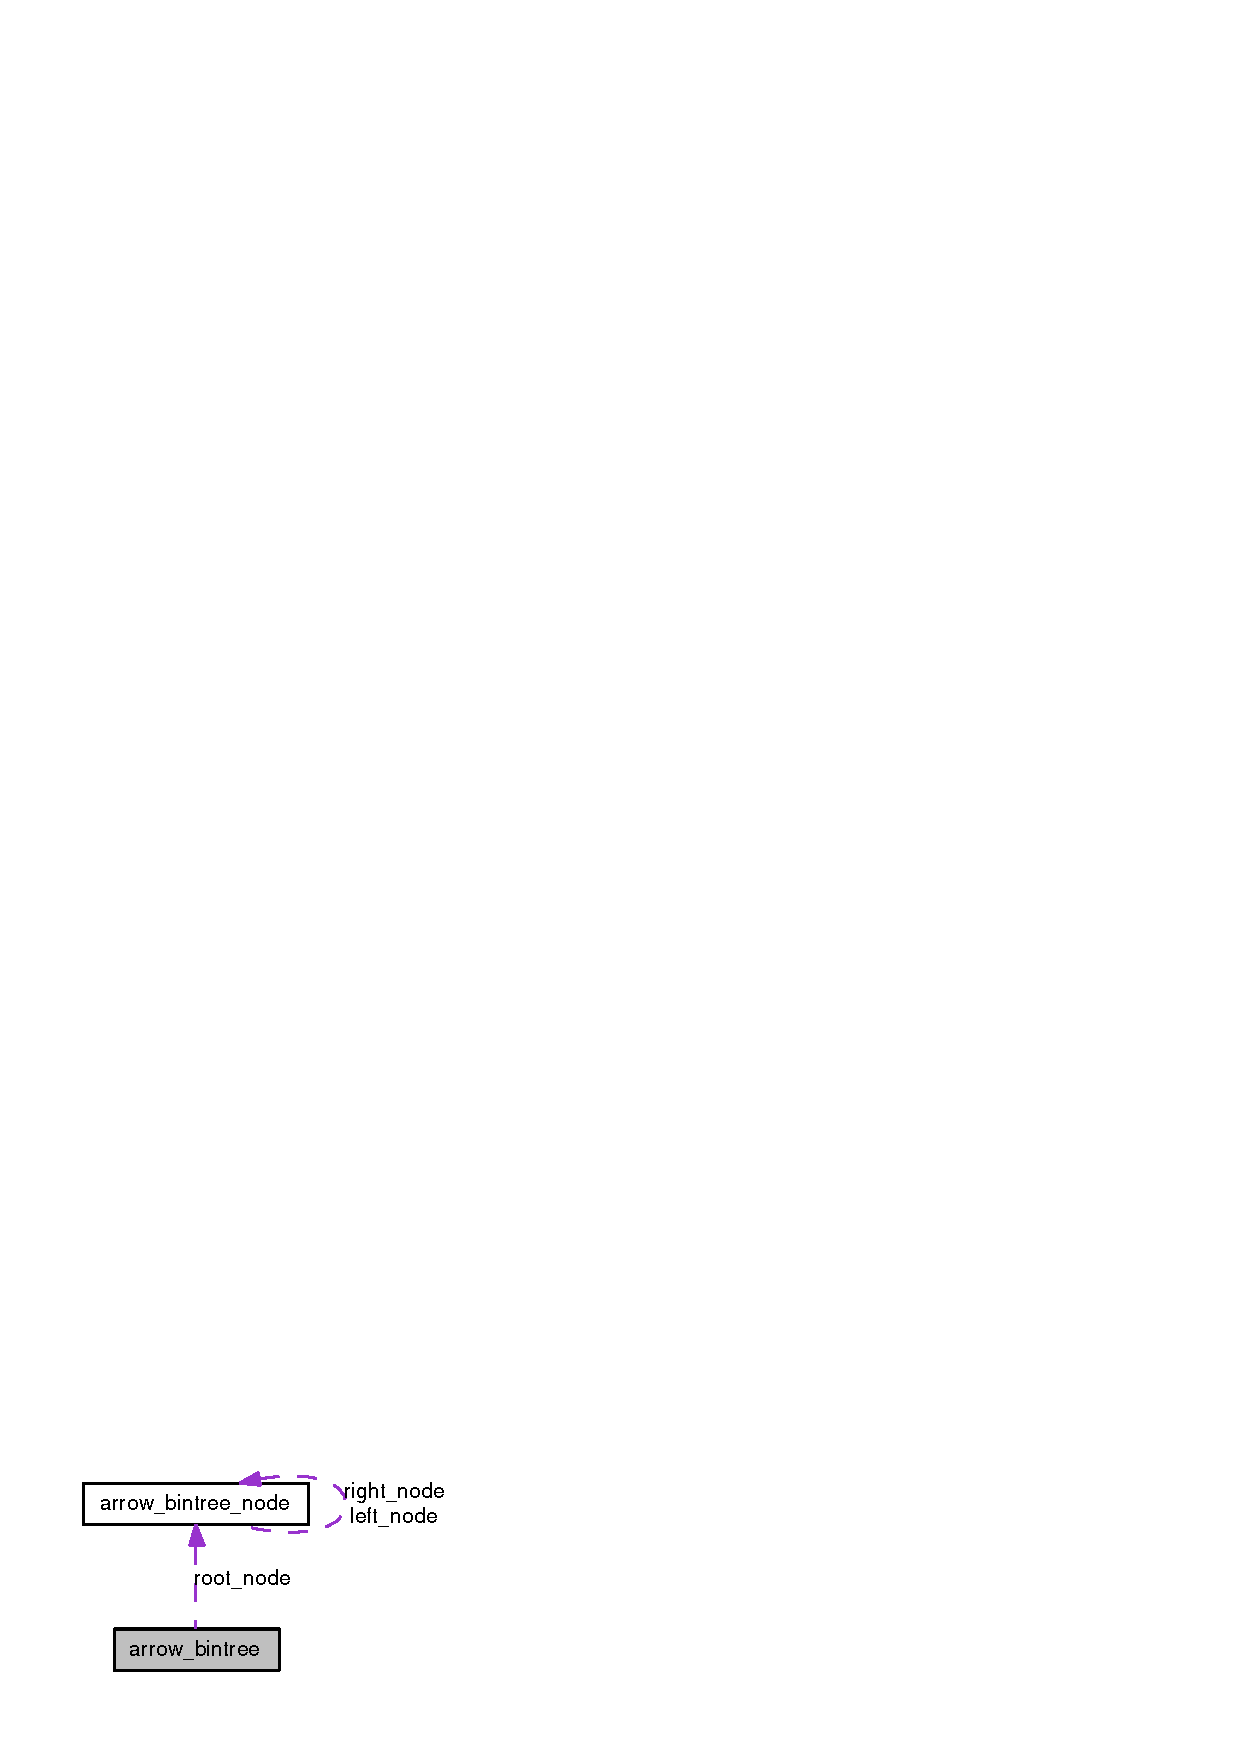
\includegraphics[width=109pt]{structarrow__bintree__coll__graph}
\end{center}
\end{figure}
\subsection*{Data Fields}
\begin{CompactItemize}
\item 
struct \hyperlink{structarrow__bintree__node}{arrow\_\-bintree\_\-node} $\ast$ \hyperlink{structarrow__bintree_09f6d0bd6e32ae2c2f8df57a31388df6}{root\_\-node}
\item 
int \hyperlink{structarrow__bintree_7570628df0b5317cc8e240499ba12974}{size}
\end{CompactItemize}


\subsection{Detailed Description}
Binary tree data structure. 

Definition at line 82 of file common.h.

\subsection{Field Documentation}
\hypertarget{structarrow__bintree_09f6d0bd6e32ae2c2f8df57a31388df6}{
\index{arrow\_\-bintree@{arrow\_\-bintree}!root\_\-node@{root\_\-node}}
\index{root\_\-node@{root\_\-node}!arrow_bintree@{arrow\_\-bintree}}
\subsubsection{\setlength{\rightskip}{0pt plus 5cm}struct {\bf arrow\_\-bintree\_\-node}$\ast$ {\bf arrow\_\-bintree::root\_\-node}\hspace{0.3cm}{\tt  \mbox{[}read\mbox{]}}}}
\label{structarrow__bintree_09f6d0bd6e32ae2c2f8df57a31388df6}


root node of tree 

Definition at line 84 of file common.h.

Referenced by arrow\_\-bintree\_\-destruct(), arrow\_\-bintree\_\-init(), arrow\_\-bintree\_\-insert(), and arrow\_\-bintree\_\-to\_\-array().\hypertarget{structarrow__bintree_7570628df0b5317cc8e240499ba12974}{
\index{arrow\_\-bintree@{arrow\_\-bintree}!size@{size}}
\index{size@{size}!arrow_bintree@{arrow\_\-bintree}}
\subsubsection{\setlength{\rightskip}{0pt plus 5cm}int {\bf arrow\_\-bintree::size}}}
\label{structarrow__bintree_7570628df0b5317cc8e240499ba12974}


size of tree 

Definition at line 85 of file common.h.

Referenced by arrow\_\-bintree\_\-destruct(), arrow\_\-bintree\_\-init(), arrow\_\-bintree\_\-insert(), arrow\_\-bintree\_\-to\_\-new\_\-array(), arrow\_\-problem\_\-info\_\-get(), and insert\_\-at().

The documentation for this struct was generated from the following file:\begin{CompactItemize}
\item 
include/\hyperlink{common_8h}{common.h}\end{CompactItemize}

\hypertarget{structarrow__bintree__node}{
\section{arrow\_\-bintree\_\-node Struct Reference}
\label{structarrow__bintree__node}\index{arrow\_\-bintree\_\-node@{arrow\_\-bintree\_\-node}}
}
Binary tree node.  


{\tt \#include $<$arrow.h$>$}

Collaboration diagram for arrow\_\-bintree\_\-node:\nopagebreak
\begin{figure}[H]
\begin{center}
\leavevmode
\includegraphics[width=109pt]{structarrow__bintree__node__coll__graph}
\end{center}
\end{figure}
\subsection*{Data Fields}
\begin{CompactItemize}
\item 
int \hyperlink{structarrow__bintree__node_de01c6e7aa823db027836d77e7ce48b6}{data}
\item 
int \hyperlink{structarrow__bintree__node_a359d3d029023fb8763af3329207ee53}{has\_\-left\_\-node}
\item 
int \hyperlink{structarrow__bintree__node_f6f8bb35c520a88841a810777e9bc186}{has\_\-right\_\-node}
\item 
struct \hyperlink{structarrow__bintree__node}{arrow\_\-bintree\_\-node} $\ast$ \hyperlink{structarrow__bintree__node_e7eb125cad02704a57796b16c49b2983}{left\_\-node}
\item 
struct \hyperlink{structarrow__bintree__node}{arrow\_\-bintree\_\-node} $\ast$ \hyperlink{structarrow__bintree__node_4875801983f2b0220212951e6c0130af}{right\_\-node}
\end{CompactItemize}


\subsection{Detailed Description}
Binary tree node. 

Definition at line 97 of file arrow.h.

\subsection{Field Documentation}
\hypertarget{structarrow__bintree__node_de01c6e7aa823db027836d77e7ce48b6}{
\index{arrow\_\-bintree\_\-node@{arrow\_\-bintree\_\-node}!data@{data}}
\index{data@{data}!arrow_bintree_node@{arrow\_\-bintree\_\-node}}
\subsubsection{\setlength{\rightskip}{0pt plus 5cm}int {\bf arrow\_\-bintree\_\-node::data}}}
\label{structarrow__bintree__node_de01c6e7aa823db027836d77e7ce48b6}


data contained in node 

Definition at line 99 of file arrow.h.

Referenced by fill\_\-array(), and insert\_\-at().\hypertarget{structarrow__bintree__node_a359d3d029023fb8763af3329207ee53}{
\index{arrow\_\-bintree\_\-node@{arrow\_\-bintree\_\-node}!has\_\-left\_\-node@{has\_\-left\_\-node}}
\index{has\_\-left\_\-node@{has\_\-left\_\-node}!arrow_bintree_node@{arrow\_\-bintree\_\-node}}
\subsubsection{\setlength{\rightskip}{0pt plus 5cm}int {\bf arrow\_\-bintree\_\-node::has\_\-left\_\-node}}}
\label{structarrow__bintree__node_a359d3d029023fb8763af3329207ee53}


true if left node exists 

Definition at line 100 of file arrow.h.

Referenced by destruct\_\-node(), fill\_\-array(), and insert\_\-at().\hypertarget{structarrow__bintree__node_f6f8bb35c520a88841a810777e9bc186}{
\index{arrow\_\-bintree\_\-node@{arrow\_\-bintree\_\-node}!has\_\-right\_\-node@{has\_\-right\_\-node}}
\index{has\_\-right\_\-node@{has\_\-right\_\-node}!arrow_bintree_node@{arrow\_\-bintree\_\-node}}
\subsubsection{\setlength{\rightskip}{0pt plus 5cm}int {\bf arrow\_\-bintree\_\-node::has\_\-right\_\-node}}}
\label{structarrow__bintree__node_f6f8bb35c520a88841a810777e9bc186}


true if right node exists 

Definition at line 101 of file arrow.h.

Referenced by destruct\_\-node(), fill\_\-array(), and insert\_\-at().\hypertarget{structarrow__bintree__node_e7eb125cad02704a57796b16c49b2983}{
\index{arrow\_\-bintree\_\-node@{arrow\_\-bintree\_\-node}!left\_\-node@{left\_\-node}}
\index{left\_\-node@{left\_\-node}!arrow_bintree_node@{arrow\_\-bintree\_\-node}}
\subsubsection{\setlength{\rightskip}{0pt plus 5cm}struct {\bf arrow\_\-bintree\_\-node}$\ast$ {\bf arrow\_\-bintree\_\-node::left\_\-node}\hspace{0.3cm}{\tt  \mbox{[}read\mbox{]}}}}
\label{structarrow__bintree__node_e7eb125cad02704a57796b16c49b2983}


left node 

Definition at line 102 of file arrow.h.

Referenced by destruct\_\-node(), fill\_\-array(), and insert\_\-at().\hypertarget{structarrow__bintree__node_4875801983f2b0220212951e6c0130af}{
\index{arrow\_\-bintree\_\-node@{arrow\_\-bintree\_\-node}!right\_\-node@{right\_\-node}}
\index{right\_\-node@{right\_\-node}!arrow_bintree_node@{arrow\_\-bintree\_\-node}}
\subsubsection{\setlength{\rightskip}{0pt plus 5cm}struct {\bf arrow\_\-bintree\_\-node}$\ast$ {\bf arrow\_\-bintree\_\-node::right\_\-node}\hspace{0.3cm}{\tt  \mbox{[}read\mbox{]}}}}
\label{structarrow__bintree__node_4875801983f2b0220212951e6c0130af}


right node 

Definition at line 103 of file arrow.h.

Referenced by destruct\_\-node(), fill\_\-array(), and insert\_\-at().

The documentation for this struct was generated from the following file:\begin{CompactItemize}
\item 
lib/\hyperlink{arrow_8h}{arrow.h}\end{CompactItemize}

\hypertarget{structarrow__problem}{
\section{arrow\_\-problem Struct Reference}
\label{structarrow__problem}\index{arrow\_\-problem@{arrow\_\-problem}}
}
Problem data structure.  


{\tt \#include $<$arrow.h$>$}

\subsection*{Data Fields}
\begin{CompactItemize}
\item 
int \hyperlink{structarrow__problem_de8573ddc391d06b08b65923fca693ec}{size}
\item 
CCdatagroup \hyperlink{structarrow__problem_5f04fe51bf6438b8f844c8cc06eb5ba0}{data}
\item 
int \hyperlink{structarrow__problem_8c3f4f7794c1430440658d69151b296d}{shallow}
\item 
char $\ast$ \hyperlink{structarrow__problem_4463422357e42b021b77b6e166eaf308}{name}
\item 
int($\ast$ \hyperlink{structarrow__problem_4f1f4c9ef90f240b248e8f39360da769}{get\_\-cost} )(struct \hyperlink{structarrow__problem}{arrow\_\-problem} $\ast$this, int i, int j)
\begin{CompactList}\small\item\em Returns the cost between node i and node j. \item\end{CompactList}\end{CompactItemize}


\subsection{Detailed Description}
Problem data structure. 

Definition at line 45 of file arrow.h.

\subsection{Field Documentation}
\hypertarget{structarrow__problem_de8573ddc391d06b08b65923fca693ec}{
\index{arrow\_\-problem@{arrow\_\-problem}!size@{size}}
\index{size@{size}!arrow_problem@{arrow\_\-problem}}
\subsubsection{\setlength{\rightskip}{0pt plus 5cm}int {\bf arrow\_\-problem::size}}}
\label{structarrow__problem_de8573ddc391d06b08b65923fca693ec}


problem size 

Definition at line 47 of file arrow.h.

Referenced by arrow\_\-bbssp\_\-biconnected(), arrow\_\-problem\_\-info\_\-get(), arrow\_\-problem\_\-print(), arrow\_\-problem\_\-read(), arrow\_\-tsp\_\-exact\_\-solve(), arrow\_\-tsp\_\-result\_\-init(), find\_\-art\_\-points(), and main().\hypertarget{structarrow__problem_5f04fe51bf6438b8f844c8cc06eb5ba0}{
\index{arrow\_\-problem@{arrow\_\-problem}!data@{data}}
\index{data@{data}!arrow_problem@{arrow\_\-problem}}
\subsubsection{\setlength{\rightskip}{0pt plus 5cm}CCdatagroup {\bf arrow\_\-problem::data}}}
\label{structarrow__problem_5f04fe51bf6438b8f844c8cc06eb5ba0}


Concorde data structure for problem. 

Definition at line 48 of file arrow.h.

Referenced by arrow\_\-problem\_\-destruct(), arrow\_\-problem\_\-read(), arrow\_\-tsp\_\-exact\_\-solve(), and concorde\_\-get\_\-cost().\hypertarget{structarrow__problem_8c3f4f7794c1430440658d69151b296d}{
\index{arrow\_\-problem@{arrow\_\-problem}!shallow@{shallow}}
\index{shallow@{shallow}!arrow_problem@{arrow\_\-problem}}
\subsubsection{\setlength{\rightskip}{0pt plus 5cm}int {\bf arrow\_\-problem::shallow}}}
\label{structarrow__problem_8c3f4f7794c1430440658d69151b296d}


indicates use of shallow copy of data 

Definition at line 49 of file arrow.h.

Referenced by arrow\_\-problem\_\-read().\hypertarget{structarrow__problem_4463422357e42b021b77b6e166eaf308}{
\index{arrow\_\-problem@{arrow\_\-problem}!name@{name}}
\index{name@{name}!arrow_problem@{arrow\_\-problem}}
\subsubsection{\setlength{\rightskip}{0pt plus 5cm}char$\ast$ {\bf arrow\_\-problem::name}}}
\label{structarrow__problem_4463422357e42b021b77b6e166eaf308}


name of problem (can be NULL) 

Definition at line 50 of file arrow.h.

Referenced by arrow\_\-problem\_\-read(), and arrow\_\-tsp\_\-exact\_\-solve().\hypertarget{structarrow__problem_4f1f4c9ef90f240b248e8f39360da769}{
\index{arrow\_\-problem@{arrow\_\-problem}!get\_\-cost@{get\_\-cost}}
\index{get\_\-cost@{get\_\-cost}!arrow_problem@{arrow\_\-problem}}
\subsubsection{\setlength{\rightskip}{0pt plus 5cm}int($\ast$ {\bf arrow\_\-problem::get\_\-cost})(struct {\bf arrow\_\-problem} $\ast$this, int i, int j)}}
\label{structarrow__problem_4f1f4c9ef90f240b248e8f39360da769}


Returns the cost between node i and node j. 

\begin{Desc}
\item[Parameters:]
\begin{description}
\item[{\em this}]\mbox{[}in\mbox{]} problem data \item[{\em i}]\mbox{[}in\mbox{]} node i \item[{\em j}]\mbox{[}in\mbox{]} node j \end{description}
\end{Desc}
\begin{Desc}
\item[Returns:]cost between node i and j. \end{Desc}


Referenced by arrow\_\-problem\_\-info\_\-get(), arrow\_\-problem\_\-print(), arrow\_\-problem\_\-read(), find\_\-art\_\-points(), and main().

The documentation for this struct was generated from the following file:\begin{CompactItemize}
\item 
lib/\hyperlink{arrow_8h}{arrow.h}\end{CompactItemize}

\hypertarget{structarrow__problem__info}{
\section{arrow\_\-problem\_\-info Struct Reference}
\label{structarrow__problem__info}\index{arrow\_\-problem\_\-info@{arrow\_\-problem\_\-info}}
}
Problem information data structure.  


{\tt \#include $<$common.h$>$}

Collaboration diagram for arrow\_\-problem\_\-info:\nopagebreak
\begin{figure}[H]
\begin{center}
\leavevmode
\includegraphics[width=63pt]{structarrow__problem__info__coll__graph}
\end{center}
\end{figure}
\subsection*{Data Fields}
\begin{CompactItemize}
\item 
int $\ast$ \hyperlink{structarrow__problem__info_7c9472312d7057fb9d74eb5579930216}{cost\_\-list}
\item 
int \hyperlink{structarrow__problem__info_54bbdc187af19361072480b45016f171}{cost\_\-list\_\-length}
\item 
int \hyperlink{structarrow__problem__info_46fabcc0ccd3a732cebb014331d4eeb5}{min\_\-cost}
\item 
int \hyperlink{structarrow__problem__info_724060f3be25521cca761899913c2776}{max\_\-cost}
\item 
\hyperlink{structarrow__hash}{arrow\_\-hash} \hyperlink{structarrow__problem__info_d62672139bdce70b23d8c72ecd96ff0d}{hash}
\end{CompactItemize}


\subsection{Detailed Description}
Problem information data structure. 

Definition at line 462 of file common.h.

\subsection{Field Documentation}
\hypertarget{structarrow__problem__info_7c9472312d7057fb9d74eb5579930216}{
\index{arrow\_\-problem\_\-info@{arrow\_\-problem\_\-info}!cost\_\-list@{cost\_\-list}}
\index{cost\_\-list@{cost\_\-list}!arrow_problem_info@{arrow\_\-problem\_\-info}}
\subsubsection{\setlength{\rightskip}{0pt plus 5cm}int$\ast$ {\bf arrow\_\-problem\_\-info::cost\_\-list}}}
\label{structarrow__problem__info_7c9472312d7057fb9d74eb5579930216}


sorted list of unique costs from problem. 

Definition at line 464 of file common.h.

Referenced by arrow\_\-bap\_\-solve(), arrow\_\-bbssp\_\-solve(), arrow\_\-bscssp\_\-solve(), arrow\_\-btsp\_\-solve(), arrow\_\-cbap\_\-solve(), arrow\_\-problem\_\-info\_\-cost\_\-index(), arrow\_\-problem\_\-info\_\-destruct(), arrow\_\-problem\_\-info\_\-get(), and main().\hypertarget{structarrow__problem__info_54bbdc187af19361072480b45016f171}{
\index{arrow\_\-problem\_\-info@{arrow\_\-problem\_\-info}!cost\_\-list\_\-length@{cost\_\-list\_\-length}}
\index{cost\_\-list\_\-length@{cost\_\-list\_\-length}!arrow_problem_info@{arrow\_\-problem\_\-info}}
\subsubsection{\setlength{\rightskip}{0pt plus 5cm}int {\bf arrow\_\-problem\_\-info::cost\_\-list\_\-length}}}
\label{structarrow__problem__info_54bbdc187af19361072480b45016f171}


length of cost list. 

Definition at line 465 of file common.h.

Referenced by arrow\_\-bap\_\-solve(), arrow\_\-bbssp\_\-solve(), arrow\_\-bscssp\_\-solve(), arrow\_\-btsp\_\-fun\_\-cbtsp\_\-shake(), arrow\_\-btsp\_\-solve(), arrow\_\-cbap\_\-solve(), arrow\_\-problem\_\-info\_\-cost\_\-index(), arrow\_\-problem\_\-info\_\-get(), and main().\hypertarget{structarrow__problem__info_46fabcc0ccd3a732cebb014331d4eeb5}{
\index{arrow\_\-problem\_\-info@{arrow\_\-problem\_\-info}!min\_\-cost@{min\_\-cost}}
\index{min\_\-cost@{min\_\-cost}!arrow_problem_info@{arrow\_\-problem\_\-info}}
\subsubsection{\setlength{\rightskip}{0pt plus 5cm}int {\bf arrow\_\-problem\_\-info::min\_\-cost}}}
\label{structarrow__problem__info_46fabcc0ccd3a732cebb014331d4eeb5}


smallest cost in problem. 

Definition at line 466 of file common.h.

Referenced by arrow\_\-problem\_\-info\_\-get(), and main().\hypertarget{structarrow__problem__info_724060f3be25521cca761899913c2776}{
\index{arrow\_\-problem\_\-info@{arrow\_\-problem\_\-info}!max\_\-cost@{max\_\-cost}}
\index{max\_\-cost@{max\_\-cost}!arrow_problem_info@{arrow\_\-problem\_\-info}}
\subsubsection{\setlength{\rightskip}{0pt plus 5cm}int {\bf arrow\_\-problem\_\-info::max\_\-cost}}}
\label{structarrow__problem__info_724060f3be25521cca761899913c2776}


largest cost in problem. 

Definition at line 467 of file common.h.

Referenced by arrow\_\-cbst\_\-mst\_\-solve(), arrow\_\-cbst\_\-solve(), arrow\_\-problem\_\-info\_\-get(), and main().\hypertarget{structarrow__problem__info_d62672139bdce70b23d8c72ecd96ff0d}{
\index{arrow\_\-problem\_\-info@{arrow\_\-problem\_\-info}!hash@{hash}}
\index{hash@{hash}!arrow_problem_info@{arrow\_\-problem\_\-info}}
\subsubsection{\setlength{\rightskip}{0pt plus 5cm}{\bf arrow\_\-hash} {\bf arrow\_\-problem\_\-info::hash}}}
\label{structarrow__problem__info_d62672139bdce70b23d8c72ecd96ff0d}


hash table structure 

Definition at line 468 of file common.h.

Referenced by arrow\_\-problem\_\-info\_\-cost\_\-index(), arrow\_\-problem\_\-info\_\-destruct(), arrow\_\-problem\_\-info\_\-get(), and main().

The documentation for this struct was generated from the following file:\begin{CompactItemize}
\item 
include/\hyperlink{common_8h}{common.h}\end{CompactItemize}

\hypertarget{structarrow__tsp__lk__params}{
\section{arrow\_\-tsp\_\-lk\_\-params Struct Reference}
\label{structarrow__tsp__lk__params}\index{arrow\_\-tsp\_\-lk\_\-params@{arrow\_\-tsp\_\-lk\_\-params}}
}
LK algorithm parameters.  


{\tt \#include $<$arrow.h$>$}

\subsection*{Data Fields}
\begin{CompactItemize}
\item 
int \hyperlink{structarrow__tsp__lk__params_ad3822d8c0e5d78b09618dbf716c3a4a}{random\_\-restarts}
\item 
int \hyperlink{structarrow__tsp__lk__params_ec5d500e1f1d7dabbbe0d1aae2abfcf8}{stall\_\-count}
\item 
int \hyperlink{structarrow__tsp__lk__params_9744a2fb89bca6b678fec9a6a17255ea}{kicks}
\item 
int \hyperlink{structarrow__tsp__lk__params_5b724dc268faa478b5b3e14c19abdc2a}{kick\_\-type}
\item 
double \hyperlink{structarrow__tsp__lk__params_22355808165edb6033ca771b88917cf5}{time\_\-bound}
\item 
double \hyperlink{structarrow__tsp__lk__params_36fb446a90e9b4c76702bd93f00357ea}{length\_\-bound}
\item 
int $\ast$ \hyperlink{structarrow__tsp__lk__params_1684519ac0bb6e529707b59f6cd7d528}{initial\_\-tour}
\end{CompactItemize}


\subsection{Detailed Description}
LK algorithm parameters. 

Definition at line 142 of file arrow.h.

\subsection{Field Documentation}
\hypertarget{structarrow__tsp__lk__params_ad3822d8c0e5d78b09618dbf716c3a4a}{
\index{arrow\_\-tsp\_\-lk\_\-params@{arrow\_\-tsp\_\-lk\_\-params}!random\_\-restarts@{random\_\-restarts}}
\index{random\_\-restarts@{random\_\-restarts}!arrow_tsp_lk_params@{arrow\_\-tsp\_\-lk\_\-params}}
\subsubsection{\setlength{\rightskip}{0pt plus 5cm}int {\bf arrow\_\-tsp\_\-lk\_\-params::random\_\-restarts}}}
\label{structarrow__tsp__lk__params_ad3822d8c0e5d78b09618dbf716c3a4a}


the number of random restarts to perform 

Definition at line 144 of file arrow.h.

Referenced by arrow\_\-tsp\_\-lk\_\-params\_\-init(), arrow\_\-tsp\_\-lk\_\-solve(), and main().\hypertarget{structarrow__tsp__lk__params_ec5d500e1f1d7dabbbe0d1aae2abfcf8}{
\index{arrow\_\-tsp\_\-lk\_\-params@{arrow\_\-tsp\_\-lk\_\-params}!stall\_\-count@{stall\_\-count}}
\index{stall\_\-count@{stall\_\-count}!arrow_tsp_lk_params@{arrow\_\-tsp\_\-lk\_\-params}}
\subsubsection{\setlength{\rightskip}{0pt plus 5cm}int {\bf arrow\_\-tsp\_\-lk\_\-params::stall\_\-count}}}
\label{structarrow__tsp__lk__params_ec5d500e1f1d7dabbbe0d1aae2abfcf8}


the max number of 4-swap kicks to perform without making progress 

Definition at line 145 of file arrow.h.

Referenced by arrow\_\-tsp\_\-lk\_\-params\_\-init(), arrow\_\-tsp\_\-lk\_\-solve(), and main().\hypertarget{structarrow__tsp__lk__params_9744a2fb89bca6b678fec9a6a17255ea}{
\index{arrow\_\-tsp\_\-lk\_\-params@{arrow\_\-tsp\_\-lk\_\-params}!kicks@{kicks}}
\index{kicks@{kicks}!arrow_tsp_lk_params@{arrow\_\-tsp\_\-lk\_\-params}}
\subsubsection{\setlength{\rightskip}{0pt plus 5cm}int {\bf arrow\_\-tsp\_\-lk\_\-params::kicks}}}
\label{structarrow__tsp__lk__params_9744a2fb89bca6b678fec9a6a17255ea}


the number of 4-swap kicks to perform 

Definition at line 147 of file arrow.h.

Referenced by arrow\_\-tsp\_\-lk\_\-params\_\-init(), arrow\_\-tsp\_\-lk\_\-solve(), and main().\hypertarget{structarrow__tsp__lk__params_5b724dc268faa478b5b3e14c19abdc2a}{
\index{arrow\_\-tsp\_\-lk\_\-params@{arrow\_\-tsp\_\-lk\_\-params}!kick\_\-type@{kick\_\-type}}
\index{kick\_\-type@{kick\_\-type}!arrow_tsp_lk_params@{arrow\_\-tsp\_\-lk\_\-params}}
\subsubsection{\setlength{\rightskip}{0pt plus 5cm}int {\bf arrow\_\-tsp\_\-lk\_\-params::kick\_\-type}}}
\label{structarrow__tsp__lk__params_5b724dc268faa478b5b3e14c19abdc2a}


the type of kick: one of CC\_\-LK\_\-RANDOM\_\-KICK, CC\_\-LK\_\-GEOMETRIC\_\-KICK, or CC\_\-LK\_\-CLOSE\_\-KICK; see Concorde documentation for more info 

Definition at line 148 of file arrow.h.

Referenced by arrow\_\-tsp\_\-lk\_\-params\_\-init(), and arrow\_\-tsp\_\-lk\_\-solve().\hypertarget{structarrow__tsp__lk__params_22355808165edb6033ca771b88917cf5}{
\index{arrow\_\-tsp\_\-lk\_\-params@{arrow\_\-tsp\_\-lk\_\-params}!time\_\-bound@{time\_\-bound}}
\index{time\_\-bound@{time\_\-bound}!arrow_tsp_lk_params@{arrow\_\-tsp\_\-lk\_\-params}}
\subsubsection{\setlength{\rightskip}{0pt plus 5cm}double {\bf arrow\_\-tsp\_\-lk\_\-params::time\_\-bound}}}
\label{structarrow__tsp__lk__params_22355808165edb6033ca771b88917cf5}


stop after this running time reached; set to 0 to have no time bound, must be positive 

Definition at line 151 of file arrow.h.

Referenced by arrow\_\-tsp\_\-lk\_\-params\_\-init(), and arrow\_\-tsp\_\-lk\_\-solve().\hypertarget{structarrow__tsp__lk__params_36fb446a90e9b4c76702bd93f00357ea}{
\index{arrow\_\-tsp\_\-lk\_\-params@{arrow\_\-tsp\_\-lk\_\-params}!length\_\-bound@{length\_\-bound}}
\index{length\_\-bound@{length\_\-bound}!arrow_tsp_lk_params@{arrow\_\-tsp\_\-lk\_\-params}}
\subsubsection{\setlength{\rightskip}{0pt plus 5cm}double {\bf arrow\_\-tsp\_\-lk\_\-params::length\_\-bound}}}
\label{structarrow__tsp__lk__params_36fb446a90e9b4c76702bd93f00357ea}


stop after finding tour of this length; must be non-negative 

Definition at line 153 of file arrow.h.

Referenced by arrow\_\-tsp\_\-lk\_\-params\_\-init(), arrow\_\-tsp\_\-lk\_\-solve(), and main().\hypertarget{structarrow__tsp__lk__params_1684519ac0bb6e529707b59f6cd7d528}{
\index{arrow\_\-tsp\_\-lk\_\-params@{arrow\_\-tsp\_\-lk\_\-params}!initial\_\-tour@{initial\_\-tour}}
\index{initial\_\-tour@{initial\_\-tour}!arrow_tsp_lk_params@{arrow\_\-tsp\_\-lk\_\-params}}
\subsubsection{\setlength{\rightskip}{0pt plus 5cm}int$\ast$ {\bf arrow\_\-tsp\_\-lk\_\-params::initial\_\-tour}}}
\label{structarrow__tsp__lk__params_1684519ac0bb6e529707b59f6cd7d528}


initial tour (may be NULL) 

Definition at line 155 of file arrow.h.

Referenced by arrow\_\-tsp\_\-lk\_\-params\_\-destruct(), arrow\_\-tsp\_\-lk\_\-params\_\-init(), and arrow\_\-tsp\_\-lk\_\-solve().

The documentation for this struct was generated from the following file:\begin{CompactItemize}
\item 
lib/\hyperlink{arrow_8h}{arrow.h}\end{CompactItemize}

\hypertarget{structarrow__tsp__result}{
\section{arrow\_\-tsp\_\-result Struct Reference}
\label{structarrow__tsp__result}\index{arrow\_\-tsp\_\-result@{arrow\_\-tsp\_\-result}}
}
TSP result (including result from LK heuristic).  


{\tt \#include $<$arrow.h$>$}

\subsection*{Data Fields}
\begin{CompactItemize}
\item 
int \hyperlink{structarrow__tsp__result_b85143df6ecc70032db7411a1aa3192a}{found\_\-tour}
\item 
double \hyperlink{structarrow__tsp__result_93a335ce86270dd455185d22ea5fd4ab}{tour\_\-length}
\item 
int $\ast$ \hyperlink{structarrow__tsp__result_48433b03146d6ca3423a555ea2139d52}{tour}
\item 
double \hyperlink{structarrow__tsp__result_82ea7aa0320d932892602d34339a9276}{total\_\-time}
\end{CompactItemize}


\subsection{Detailed Description}
TSP result (including result from LK heuristic). 

Definition at line 216 of file arrow.h.

\subsection{Field Documentation}
\hypertarget{structarrow__tsp__result_b85143df6ecc70032db7411a1aa3192a}{
\index{arrow\_\-tsp\_\-result@{arrow\_\-tsp\_\-result}!found\_\-tour@{found\_\-tour}}
\index{found\_\-tour@{found\_\-tour}!arrow_tsp_result@{arrow\_\-tsp\_\-result}}
\subsubsection{\setlength{\rightskip}{0pt plus 5cm}int {\bf arrow\_\-tsp\_\-result::found\_\-tour}}}
\label{structarrow__tsp__result_b85143df6ecc70032db7411a1aa3192a}


true if a tour was found, false otherwise 

Definition at line 218 of file arrow.h.

Referenced by arrow\_\-tsp\_\-exact\_\-solve(), and arrow\_\-tsp\_\-result\_\-init().\hypertarget{structarrow__tsp__result_93a335ce86270dd455185d22ea5fd4ab}{
\index{arrow\_\-tsp\_\-result@{arrow\_\-tsp\_\-result}!tour\_\-length@{tour\_\-length}}
\index{tour\_\-length@{tour\_\-length}!arrow_tsp_result@{arrow\_\-tsp\_\-result}}
\subsubsection{\setlength{\rightskip}{0pt plus 5cm}double {\bf arrow\_\-tsp\_\-result::tour\_\-length}}}
\label{structarrow__tsp__result_93a335ce86270dd455185d22ea5fd4ab}


tour length 

Definition at line 219 of file arrow.h.

Referenced by arrow\_\-tsp\_\-exact\_\-solve(), and arrow\_\-tsp\_\-result\_\-init().\hypertarget{structarrow__tsp__result_48433b03146d6ca3423a555ea2139d52}{
\index{arrow\_\-tsp\_\-result@{arrow\_\-tsp\_\-result}!tour@{tour}}
\index{tour@{tour}!arrow_tsp_result@{arrow\_\-tsp\_\-result}}
\subsubsection{\setlength{\rightskip}{0pt plus 5cm}int$\ast$ {\bf arrow\_\-tsp\_\-result::tour}}}
\label{structarrow__tsp__result_48433b03146d6ca3423a555ea2139d52}


tour that was found in node-node format 

Definition at line 220 of file arrow.h.

Referenced by arrow\_\-tsp\_\-exact\_\-solve(), arrow\_\-tsp\_\-result\_\-destruct(), and arrow\_\-tsp\_\-result\_\-init().\hypertarget{structarrow__tsp__result_82ea7aa0320d932892602d34339a9276}{
\index{arrow\_\-tsp\_\-result@{arrow\_\-tsp\_\-result}!total\_\-time@{total\_\-time}}
\index{total\_\-time@{total\_\-time}!arrow_tsp_result@{arrow\_\-tsp\_\-result}}
\subsubsection{\setlength{\rightskip}{0pt plus 5cm}double {\bf arrow\_\-tsp\_\-result::total\_\-time}}}
\label{structarrow__tsp__result_82ea7aa0320d932892602d34339a9276}


total time 

Definition at line 221 of file arrow.h.

Referenced by arrow\_\-tsp\_\-exact\_\-solve(), and arrow\_\-tsp\_\-result\_\-init().

The documentation for this struct was generated from the following file:\begin{CompactItemize}
\item 
lib/\hyperlink{arrow_8h}{arrow.h}\end{CompactItemize}

\chapter{File Documentation}
\hypertarget{bin_2bbssp_8c}{
\section{bin/bbssp.c File Reference}
\label{bin_2bbssp_8c}\index{bin/bbssp.c@{bin/bbssp.c}}
}
Bottleneck Biconnected Spanning Subgraph solver.  


{\tt \#include \char`\"{}common.h\char`\"{}}\par
{\tt \#include \char`\"{}lb.h\char`\"{}}\par
\subsection*{Defines}
\begin{CompactItemize}
\item 
\#define \hyperlink{bin_2bbssp_8c_9b58b2c4af931c8486a986c9deca40f5}{NUM\_\-OPTS}~5
\end{CompactItemize}
\subsection*{Functions}
\begin{CompactItemize}
\item 
int \hyperlink{bin_2bbssp_8c_0ddf1224851353fc92bfbff6f499fa97}{main} (int argc, char $\ast$argv\mbox{[}$\,$\mbox{]})
\end{CompactItemize}
\subsection*{Variables}
\begin{CompactItemize}
\item 
char $\ast$ \hyperlink{bin_2bbssp_8c_289c5900d90626d909f0a85d5a0ed61d}{program\_\-name}
\item 
char $\ast$ \hyperlink{bin_2bbssp_8c_a4f3a15de34c409bdec6ceacf93078ed}{input\_\-file} = NULL
\item 
char $\ast$ \hyperlink{bin_2bbssp_8c_bf4e392494984c6ef8259268eb1fe421}{xml\_\-file} = NULL
\item 
int \hyperlink{bin_2bbssp_8c_786cdab056142ae00a268cabebd5ced7}{solve\_\-mstsp} = ARROW\_\-FALSE
\item 
int \hyperlink{bin_2bbssp_8c_eb8ae508d4fe942c0d6ca38d1470ac25}{sym\_\-transform} = ARROW\_\-FALSE
\item 
int \hyperlink{bin_2bbssp_8c_7298da576a5b127d04b4c46b3bc78821}{deep\_\-copy} = ARROW\_\-FALSE
\item 
\hyperlink{structarrow__option}{arrow\_\-option} \hyperlink{bin_2bbssp_8c_cea6a9709d519c143f30db401a0d0c72}{options} \mbox{[}NUM\_\-OPTS\mbox{]}
\item 
char $\ast$ \hyperlink{bin_2bbssp_8c_3aad16fd4bea1b9717f232ea75ad6449}{desc} = \char`\"{}Bottleneck biconnected spanning subgraph solver\char`\"{}
\item 
char $\ast$ \hyperlink{bin_2bbssp_8c_adebe2487a2c5240ab6cd02c83add0bf}{usage} = \char`\"{}-i tsplib.tsp \mbox{[}\hyperlink{tourinfo_8c_cea6a9709d519c143f30db401a0d0c72}{options}\mbox{]} \char`\"{}
\end{CompactItemize}


\subsection{Detailed Description}
Bottleneck Biconnected Spanning Subgraph solver. 

Solves the bottleneck biconnected spanning subgraph problem (BBSSP) problem on the given input file.

\begin{Desc}
\item[Author:]John LaRusic \end{Desc}


Definition in file \hyperlink{bin_2bbssp_8c-source}{bbssp.c}.

\subsection{Define Documentation}
\hypertarget{bin_2bbssp_8c_9b58b2c4af931c8486a986c9deca40f5}{
\index{bin/bbssp.c@{bin/bbssp.c}!NUM\_\-OPTS@{NUM\_\-OPTS}}
\index{NUM\_\-OPTS@{NUM\_\-OPTS}!bin/bbssp.c@{bin/bbssp.c}}
\subsubsection[{NUM\_\-OPTS}]{\setlength{\rightskip}{0pt plus 5cm}\#define NUM\_\-OPTS~5}}
\label{bin_2bbssp_8c_9b58b2c4af931c8486a986c9deca40f5}




Definition at line 22 of file bbssp.c.

\subsection{Function Documentation}
\hypertarget{bin_2bbssp_8c_0ddf1224851353fc92bfbff6f499fa97}{
\index{bin/bbssp.c@{bin/bbssp.c}!main@{main}}
\index{main@{main}!bin/bbssp.c@{bin/bbssp.c}}
\subsubsection[{main}]{\setlength{\rightskip}{0pt plus 5cm}int main (int {\em argc}, \/  char $\ast$ {\em argv}\mbox{[}$\,$\mbox{]})}}
\label{bin_2bbssp_8c_0ddf1224851353fc92bfbff6f499fa97}




Definition at line 41 of file bbssp.c.

References arrow\_\-bbssp\_\-solve(), ARROW\_\-FAILURE, ARROW\_\-FALSE, arrow\_\-options\_\-parse(), arrow\_\-print\_\-error, arrow\_\-problem\_\-abtsp\_\-to\_\-sbtsp(), arrow\_\-problem\_\-destruct(), arrow\_\-problem\_\-info\_\-destruct(), arrow\_\-problem\_\-info\_\-get(), arrow\_\-problem\_\-max\_\-cost(), arrow\_\-problem\_\-mstsp\_\-to\_\-btsp(), arrow\_\-problem\_\-read(), ARROW\_\-SUCCESS, arrow\_\-util\_\-print\_\-program\_\-args(), deep\_\-copy, desc, input\_\-file, arrow\_\-problem\_\-info::max\_\-cost, NUM\_\-OPTS, arrow\_\-bound\_\-result::obj\_\-value, arrow\_\-problem::size, solve\_\-mstsp, sym\_\-transform, arrow\_\-problem::symmetric, arrow\_\-bound\_\-result::total\_\-time, usage, and xml\_\-file.

\subsection{Variable Documentation}
\hypertarget{bin_2bbssp_8c_7298da576a5b127d04b4c46b3bc78821}{
\index{bin/bbssp.c@{bin/bbssp.c}!deep\_\-copy@{deep\_\-copy}}
\index{deep\_\-copy@{deep\_\-copy}!bin/bbssp.c@{bin/bbssp.c}}
\subsubsection[{deep\_\-copy}]{\setlength{\rightskip}{0pt plus 5cm}int {\bf deep\_\-copy} = ARROW\_\-FALSE}}
\label{bin_2bbssp_8c_7298da576a5b127d04b4c46b3bc78821}




Definition at line 19 of file bbssp.c.\hypertarget{bin_2bbssp_8c_3aad16fd4bea1b9717f232ea75ad6449}{
\index{bin/bbssp.c@{bin/bbssp.c}!desc@{desc}}
\index{desc@{desc}!bin/bbssp.c@{bin/bbssp.c}}
\subsubsection[{desc}]{\setlength{\rightskip}{0pt plus 5cm}char$\ast$ {\bf desc} = \char`\"{}Bottleneck biconnected spanning subgraph solver\char`\"{}}}
\label{bin_2bbssp_8c_3aad16fd4bea1b9717f232ea75ad6449}




Definition at line 36 of file bbssp.c.\hypertarget{bin_2bbssp_8c_a4f3a15de34c409bdec6ceacf93078ed}{
\index{bin/bbssp.c@{bin/bbssp.c}!input\_\-file@{input\_\-file}}
\index{input\_\-file@{input\_\-file}!bin/bbssp.c@{bin/bbssp.c}}
\subsubsection[{input\_\-file}]{\setlength{\rightskip}{0pt plus 5cm}char$\ast$ {\bf input\_\-file} = NULL}}
\label{bin_2bbssp_8c_a4f3a15de34c409bdec6ceacf93078ed}


Given input TSPLIB file 

Definition at line 15 of file bbssp.c.\hypertarget{bin_2bbssp_8c_cea6a9709d519c143f30db401a0d0c72}{
\index{bin/bbssp.c@{bin/bbssp.c}!options@{options}}
\index{options@{options}!bin/bbssp.c@{bin/bbssp.c}}
\subsubsection[{options}]{\setlength{\rightskip}{0pt plus 5cm}{\bf arrow\_\-option} {\bf options}\mbox{[}NUM\_\-OPTS\mbox{]}}}
\label{bin_2bbssp_8c_cea6a9709d519c143f30db401a0d0c72}


\textbf{Initial value:}

\begin{Code}\begin{verbatim} 
{
    {'i', "input", "TSPLIB input file", 
        ARROW_OPTION_STRING, &input_file, ARROW_TRUE, ARROW_TRUE},
    {'x', "xml", "File to write XML output to",
        ARROW_OPTION_STRING, &xml_file, ARROW_FALSE, ARROW_TRUE},
    {'m', "solve-mstsp", "solves maximum scatter TSP",
        ARROW_OPTION_INT, &solve_mstsp, ARROW_FALSE, ARROW_FALSE},
    {'s', "symmetric", "Transform asym. n city instance to sym. 2n city one",
        ARROW_OPTION_INT, &sym_transform, ARROW_FALSE, ARROW_FALSE},
    {'d', "deep-copy", "stores data in full cost-matrix",
        ARROW_OPTION_INT, &deep_copy, ARROW_FALSE, ARROW_FALSE}
}
\end{verbatim}
\end{Code}


Definition at line 23 of file bbssp.c.\hypertarget{bin_2bbssp_8c_289c5900d90626d909f0a85d5a0ed61d}{
\index{bin/bbssp.c@{bin/bbssp.c}!program\_\-name@{program\_\-name}}
\index{program\_\-name@{program\_\-name}!bin/bbssp.c@{bin/bbssp.c}}
\subsubsection[{program\_\-name}]{\setlength{\rightskip}{0pt plus 5cm}char$\ast$ {\bf program\_\-name}}}
\label{bin_2bbssp_8c_289c5900d90626d909f0a85d5a0ed61d}


Program name 

Definition at line 14 of file bbssp.c.\hypertarget{bin_2bbssp_8c_786cdab056142ae00a268cabebd5ced7}{
\index{bin/bbssp.c@{bin/bbssp.c}!solve\_\-mstsp@{solve\_\-mstsp}}
\index{solve\_\-mstsp@{solve\_\-mstsp}!bin/bbssp.c@{bin/bbssp.c}}
\subsubsection[{solve\_\-mstsp}]{\setlength{\rightskip}{0pt plus 5cm}int {\bf solve\_\-mstsp} = ARROW\_\-FALSE}}
\label{bin_2bbssp_8c_786cdab056142ae00a268cabebd5ced7}




Definition at line 17 of file bbssp.c.\hypertarget{bin_2bbssp_8c_eb8ae508d4fe942c0d6ca38d1470ac25}{
\index{bin/bbssp.c@{bin/bbssp.c}!sym\_\-transform@{sym\_\-transform}}
\index{sym\_\-transform@{sym\_\-transform}!bin/bbssp.c@{bin/bbssp.c}}
\subsubsection[{sym\_\-transform}]{\setlength{\rightskip}{0pt plus 5cm}int {\bf sym\_\-transform} = ARROW\_\-FALSE}}
\label{bin_2bbssp_8c_eb8ae508d4fe942c0d6ca38d1470ac25}




Definition at line 18 of file bbssp.c.

Referenced by main().\hypertarget{bin_2bbssp_8c_adebe2487a2c5240ab6cd02c83add0bf}{
\index{bin/bbssp.c@{bin/bbssp.c}!usage@{usage}}
\index{usage@{usage}!bin/bbssp.c@{bin/bbssp.c}}
\subsubsection[{usage}]{\setlength{\rightskip}{0pt plus 5cm}char$\ast$ {\bf usage} = \char`\"{}-i tsplib.tsp \mbox{[}{\bf options}\mbox{]} \char`\"{}}}
\label{bin_2bbssp_8c_adebe2487a2c5240ab6cd02c83add0bf}




Definition at line 37 of file bbssp.c.\hypertarget{bin_2bbssp_8c_bf4e392494984c6ef8259268eb1fe421}{
\index{bin/bbssp.c@{bin/bbssp.c}!xml\_\-file@{xml\_\-file}}
\index{xml\_\-file@{xml\_\-file}!bin/bbssp.c@{bin/bbssp.c}}
\subsubsection[{xml\_\-file}]{\setlength{\rightskip}{0pt plus 5cm}char$\ast$ {\bf xml\_\-file} = NULL}}
\label{bin_2bbssp_8c_bf4e392494984c6ef8259268eb1fe421}




Definition at line 16 of file bbssp.c.
\hypertarget{lib_2bbssp_8c}{
\section{lib/bbssp.c File Reference}
\label{lib_2bbssp_8c}\index{lib/bbssp.c@{lib/bbssp.c}}
}
Bottleneck biconnected spanning subgraph problem implemenation. 

{\tt \#include \char`\"{}arrow.h\char`\"{}}\par
\subsection*{Functions}
\begin{CompactItemize}
\item 
int \hyperlink{lib_2bbssp_8c_485f2a19b2a313bce3b255a845c8527d}{find\_\-art\_\-points} (\hyperlink{structarrow__problem}{arrow\_\-problem} $\ast$problem, int max\_\-cost, int node, int depth\_\-num, int root\_\-children, int $\ast$visited, int $\ast$depth, int $\ast$low, int $\ast$parent, int $\ast$art\_\-point)
\begin{CompactList}\small\item\em Recursively searches for articulation points in the graph using only costs less than or equal to 'max\_\-cost' out from the given node. \item\end{CompactList}\item 
int \hyperlink{lib_2bbssp_8c_ff7006ace4173927265facbe5f895cf0}{arrow\_\-bbssp\_\-solve} (\hyperlink{structarrow__problem}{arrow\_\-problem} $\ast$problem, \hyperlink{structarrow__problem__info}{arrow\_\-problem\_\-info} $\ast$info, \hyperlink{structarrow__bound__result}{arrow\_\-bound\_\-result} $\ast$result)
\begin{CompactList}\small\item\em Solves the bottleneck biconnected spanning subgraph problem (BBSSP) on the given problem. \item\end{CompactList}\item 
int \hyperlink{lib_2bbssp_8c_727cb19dd9cfa6315e1155796daef833}{arrow\_\-bbssp\_\-biconnected} (\hyperlink{structarrow__problem}{arrow\_\-problem} $\ast$problem, int max\_\-cost, int $\ast$result)
\begin{CompactList}\small\item\em Determines if the graph is biconnected using only edges with costs less than or equal to the given value. \item\end{CompactList}\end{CompactItemize}


\subsection{Detailed Description}
Bottleneck biconnected spanning subgraph problem implemenation. 

Implemenation of the bottleneck biconnected spanning subgraph problem (BBSSP) that's used as a lower bound for the Bottleneck TSP objective value.

\begin{Desc}
\item[Author:]John LaRusic \end{Desc}


Definition in file \hyperlink{lib_2bbssp_8c-source}{bbssp.c}.

\subsection{Function Documentation}
\hypertarget{lib_2bbssp_8c_727cb19dd9cfa6315e1155796daef833}{
\index{lib/bbssp.c@{lib/bbssp.c}!arrow\_\-bbssp\_\-biconnected@{arrow\_\-bbssp\_\-biconnected}}
\index{arrow\_\-bbssp\_\-biconnected@{arrow\_\-bbssp\_\-biconnected}!lib/bbssp.c@{lib/bbssp.c}}
\subsubsection{\setlength{\rightskip}{0pt plus 5cm}int arrow\_\-bbssp\_\-biconnected ({\bf arrow\_\-problem} $\ast$ {\em problem}, \/  int {\em max\_\-cost}, \/  int $\ast$ {\em result})}}
\label{lib_2bbssp_8c_727cb19dd9cfa6315e1155796daef833}


Determines if the graph is biconnected using only edges with costs less than or equal to the given value. 

\begin{Desc}
\item[Parameters:]
\begin{description}
\item[{\em problem}]\mbox{[}in\mbox{]} problem data \item[{\em max\_\-cost}]\mbox{[}in\mbox{]} value to check biconnectivity question against \item[{\em result}]\mbox{[}out\mbox{]} ARROW\_\-TRUE if biconnected, ARROW\_\-FALSE otherwise. \end{description}
\end{Desc}


Definition at line 94 of file bbssp.c.

References ARROW\_\-ERROR\_\-FATAL, ARROW\_\-FALSE, ARROW\_\-TRUE, arrow\_\-util\_\-create\_\-int\_\-array(), find\_\-art\_\-points(), and arrow\_\-problem::size.

Referenced by arrow\_\-bbssp\_\-solve().\hypertarget{lib_2bbssp_8c_ff7006ace4173927265facbe5f895cf0}{
\index{lib/bbssp.c@{lib/bbssp.c}!arrow\_\-bbssp\_\-solve@{arrow\_\-bbssp\_\-solve}}
\index{arrow\_\-bbssp\_\-solve@{arrow\_\-bbssp\_\-solve}!lib/bbssp.c@{lib/bbssp.c}}
\subsubsection{\setlength{\rightskip}{0pt plus 5cm}int arrow\_\-bbssp\_\-solve ({\bf arrow\_\-problem} $\ast$ {\em problem}, \/  {\bf arrow\_\-problem\_\-info} $\ast$ {\em info}, \/  {\bf arrow\_\-bound\_\-result} $\ast$ {\em result})}}
\label{lib_2bbssp_8c_ff7006ace4173927265facbe5f895cf0}


Solves the bottleneck biconnected spanning subgraph problem (BBSSP) on the given problem. 

\begin{Desc}
\item[Parameters:]
\begin{description}
\item[{\em problem}]\mbox{[}in\mbox{]} problem data \item[{\em info}]\mbox{[}in\mbox{]} problem info \item[{\em result}]\mbox{[}out\mbox{]} BBSSP solution \end{description}
\end{Desc}


Definition at line 44 of file bbssp.c.

References arrow\_\-bbssp\_\-biconnected(), ARROW\_\-ERROR\_\-FATAL, ARROW\_\-FAILURE, arrow\_\-print\_\-error, ARROW\_\-SUCCESS, ARROW\_\-TRUE, arrow\_\-util\_\-zeit(), arrow\_\-problem\_\-info::cost\_\-list, arrow\_\-problem\_\-info::cost\_\-list\_\-length, arrow\_\-bound\_\-result::obj\_\-value, arrow\_\-problem::symmetric, and arrow\_\-bound\_\-result::total\_\-time.

Referenced by main().\hypertarget{lib_2bbssp_8c_485f2a19b2a313bce3b255a845c8527d}{
\index{lib/bbssp.c@{lib/bbssp.c}!find\_\-art\_\-points@{find\_\-art\_\-points}}
\index{find\_\-art\_\-points@{find\_\-art\_\-points}!lib/bbssp.c@{lib/bbssp.c}}
\subsubsection{\setlength{\rightskip}{0pt plus 5cm}int find\_\-art\_\-points ({\bf arrow\_\-problem} $\ast$ {\em problem}, \/  int {\em max\_\-cost}, \/  int {\em node}, \/  int {\em depth\_\-num}, \/  int {\em root\_\-children}, \/  int $\ast$ {\em visited}, \/  int $\ast$ {\em depth}, \/  int $\ast$ {\em low}, \/  int $\ast$ {\em parent}, \/  int $\ast$ {\em art\_\-point})}}
\label{lib_2bbssp_8c_485f2a19b2a313bce3b255a845c8527d}


Recursively searches for articulation points in the graph using only costs less than or equal to 'max\_\-cost' out from the given node. 

\begin{Desc}
\item[Parameters:]
\begin{description}
\item[{\em problem}]\mbox{[}in\mbox{]} problem data structure \item[{\em max\_\-cost}]\mbox{[}in\mbox{]} the largest cost to consider as being in the graph \item[{\em node}]\mbox{[}in\mbox{]} the node to search outward from \item[{\em depth\_\-num}]\mbox{[}in\mbox{]} level at which the given node was first discovered \item[{\em root\_\-children}]\mbox{[}in\mbox{]} count of the number of children of the root \item[{\em visited}]\mbox{[}out\mbox{]} indicates if a node has been visited or not \item[{\em depth}]\mbox{[}out\mbox{]} indicates the discovery depth of a node \item[{\em low}]\mbox{[}out\mbox{]} indicates a back edge for some descendent of a node (e.g. the discovery depth of the node closest to the root and reachable from the given node by following zero or more edges downward and then at most one back edge) \item[{\em parent}]\mbox{[}out\mbox{]} indicates the closest \char`\"{}parent\char`\"{} of a node \item[{\em art\_\-point}]\mbox{[}out\mbox{]} indicates if the node is an articulation point \end{description}
\end{Desc}


Definition at line 168 of file bbssp.c.

References ARROW\_\-SUCCESS, arrow\_\-problem::get\_\-cost, and arrow\_\-problem::size.

Referenced by arrow\_\-bbssp\_\-biconnected().
\hypertarget{histogram__data_8c}{
\section{bin/histogram\_\-data.c File Reference}
\label{histogram__data_8c}\index{bin/histogram\_\-data.c@{bin/histogram\_\-data.c}}
}
Edge length histogram data collector. 

{\tt \#include \char`\"{}arrow.h\char`\"{}}\par
{\tt \#include $<$getopt.h$>$}\par


Include dependency graph for histogram\_\-data.c:\nopagebreak
\begin{figure}[H]
\begin{center}
\leavevmode
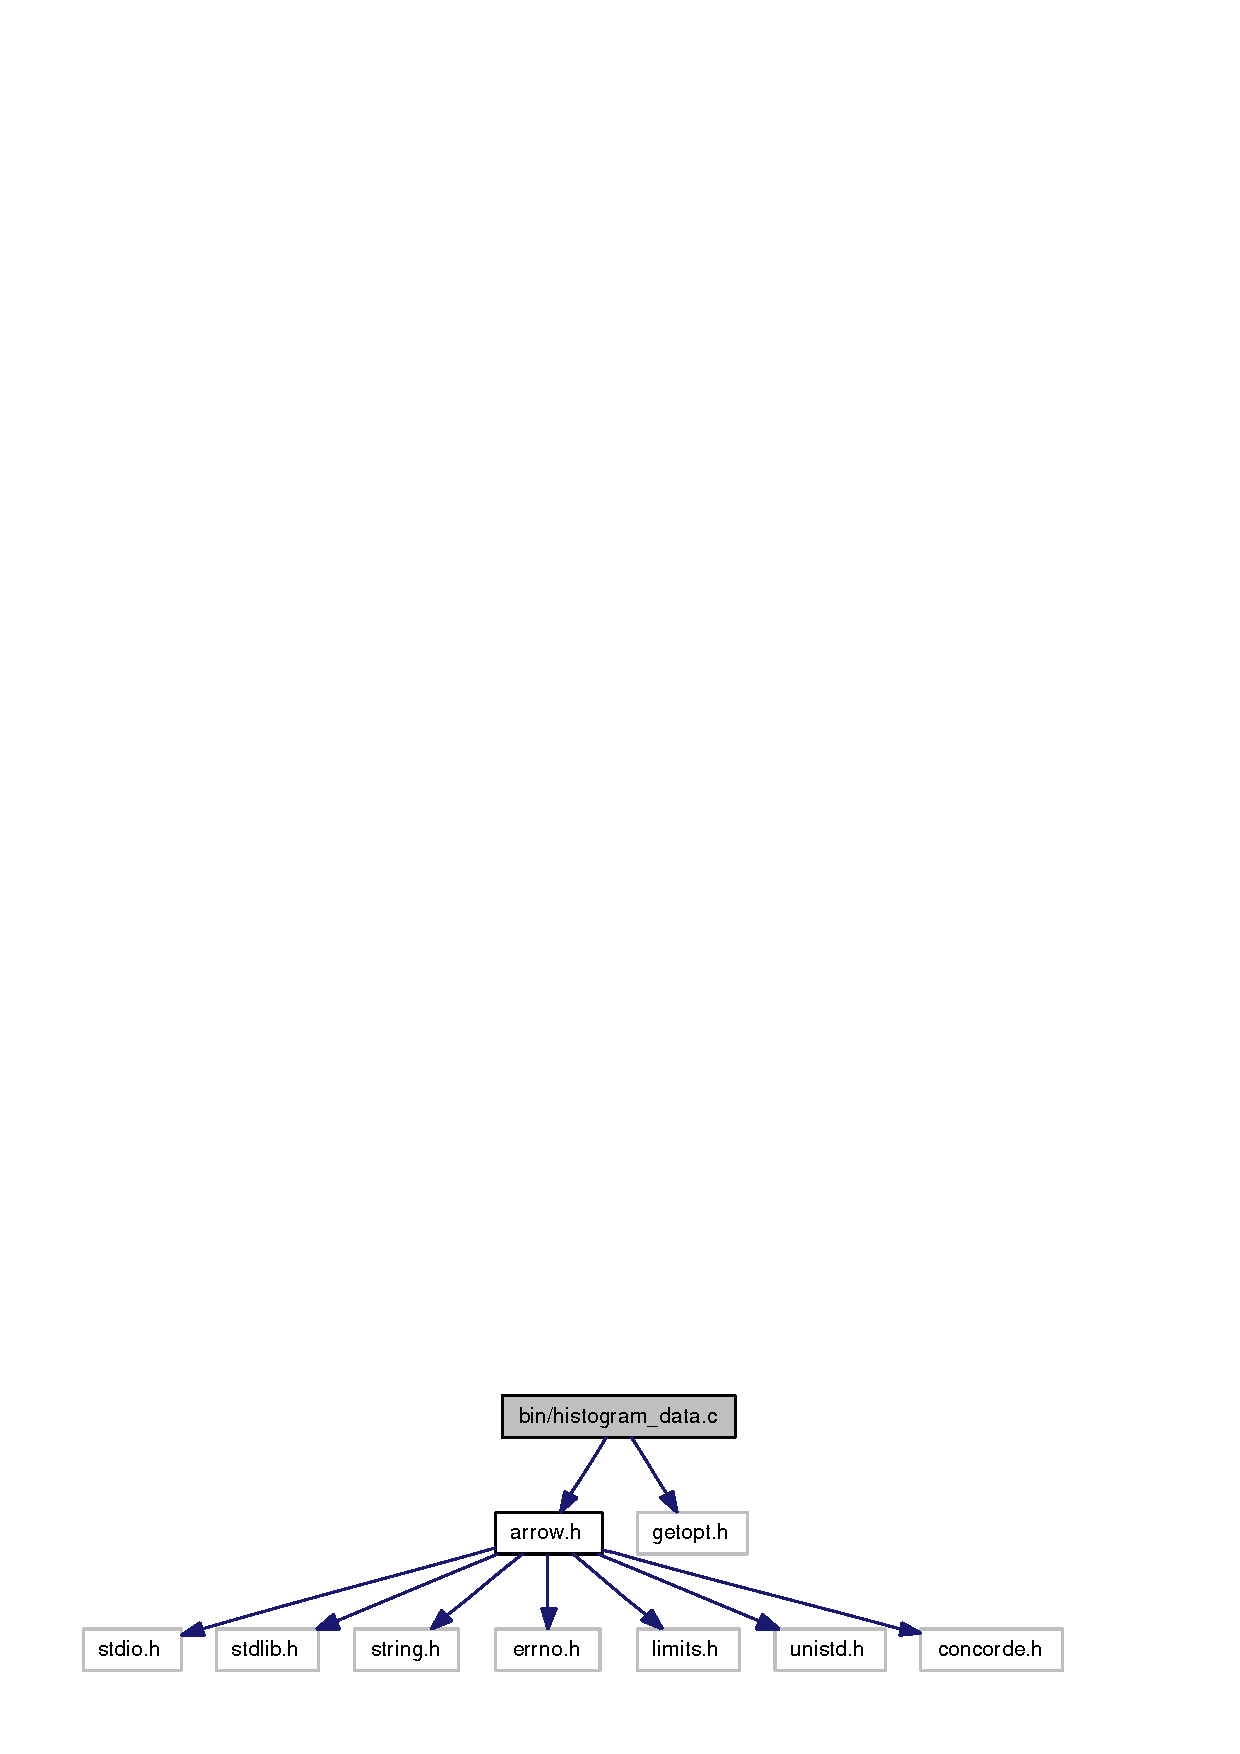
\includegraphics[width=257pt]{histogram__data_8c__incl}
\end{center}
\end{figure}
\subsection*{Functions}
\begin{CompactItemize}
\item 
void \hyperlink{histogram__data_8c_853216ac51aa181669ff4d3de74058a7}{print\_\-help} ()
\begin{CompactList}\small\item\em Prints help/usage message. \item\end{CompactList}\item 
void \hyperlink{histogram__data_8c_6302aaae12249e8ea16bfdc7de892f21}{print\_\-version} ()
\begin{CompactList}\small\item\em Prints version message. \item\end{CompactList}\item 
void \hyperlink{histogram__data_8c_e5ad5cbeccaedc03a48d3c7eaa803e79}{print\_\-usage} ()
\begin{CompactList}\small\item\em Prints usage message. \item\end{CompactList}\item 
void \hyperlink{histogram__data_8c_72d0810dad1a2062df342005c15106b9}{read\_\-args} (int argc, char $\ast$argv\mbox{[}$\,$\mbox{]})
\begin{CompactList}\small\item\em Reads program arguments. \item\end{CompactList}\item 
int \hyperlink{histogram__data_8c_0ddf1224851353fc92bfbff6f499fa97}{main} (int argc, char $\ast$argv\mbox{[}$\,$\mbox{]})
\end{CompactItemize}
\subsection*{Variables}
\begin{CompactItemize}
\item 
char $\ast$ \hyperlink{histogram__data_8c_289c5900d90626d909f0a85d5a0ed61d}{program\_\-name}
\item 
char $\ast$ \hyperlink{histogram__data_8c_a4f3a15de34c409bdec6ceacf93078ed}{input\_\-file}
\end{CompactItemize}


\subsection{Detailed Description}
Edge length histogram data collector. 

Prints out a list of every edge length present in given problem. Used in conjunction with a Python script for generating a histogram plot.

\begin{Desc}
\item[Author:]John LaRusic \end{Desc}


Definition in file \hyperlink{histogram__data_8c-source}{histogram\_\-data.c}.

\subsection{Function Documentation}
\hypertarget{histogram__data_8c_0ddf1224851353fc92bfbff6f499fa97}{
\index{histogram\_\-data.c@{histogram\_\-data.c}!main@{main}}
\index{main@{main}!histogram_data.c@{histogram\_\-data.c}}
\subsubsection{\setlength{\rightskip}{0pt plus 5cm}int main (int {\em argc}, \/  char $\ast$ {\em argv}\mbox{[}$\,$\mbox{]})}}
\label{histogram__data_8c_0ddf1224851353fc92bfbff6f499fa97}




Definition at line 45 of file histogram\_\-data.c.

References ARROW\_\-DEV\_\-NULL, arrow\_\-print\_\-error, arrow\_\-problem\_\-destruct(), arrow\_\-problem\_\-read(), arrow\_\-util\_\-redirect\_\-stdout\_\-to\_\-file(), arrow\_\-util\_\-restore\_\-stdout(), arrow\_\-problem::get\_\-cost, input\_\-file, program\_\-name, read\_\-args(), and arrow\_\-problem::size.\hypertarget{histogram__data_8c_853216ac51aa181669ff4d3de74058a7}{
\index{histogram\_\-data.c@{histogram\_\-data.c}!print\_\-help@{print\_\-help}}
\index{print\_\-help@{print\_\-help}!histogram_data.c@{histogram\_\-data.c}}
\subsubsection{\setlength{\rightskip}{0pt plus 5cm}void print\_\-help ()}}
\label{histogram__data_8c_853216ac51aa181669ff4d3de74058a7}


Prints help/usage message. 

\hypertarget{histogram__data_8c_e5ad5cbeccaedc03a48d3c7eaa803e79}{
\index{histogram\_\-data.c@{histogram\_\-data.c}!print\_\-usage@{print\_\-usage}}
\index{print\_\-usage@{print\_\-usage}!histogram_data.c@{histogram\_\-data.c}}
\subsubsection{\setlength{\rightskip}{0pt plus 5cm}void print\_\-usage ()}}
\label{histogram__data_8c_e5ad5cbeccaedc03a48d3c7eaa803e79}


Prints usage message. 

\hypertarget{histogram__data_8c_6302aaae12249e8ea16bfdc7de892f21}{
\index{histogram\_\-data.c@{histogram\_\-data.c}!print\_\-version@{print\_\-version}}
\index{print\_\-version@{print\_\-version}!histogram_data.c@{histogram\_\-data.c}}
\subsubsection{\setlength{\rightskip}{0pt plus 5cm}void print\_\-version ()}}
\label{histogram__data_8c_6302aaae12249e8ea16bfdc7de892f21}


Prints version message. 

\hypertarget{histogram__data_8c_72d0810dad1a2062df342005c15106b9}{
\index{histogram\_\-data.c@{histogram\_\-data.c}!read\_\-args@{read\_\-args}}
\index{read\_\-args@{read\_\-args}!histogram_data.c@{histogram\_\-data.c}}
\subsubsection{\setlength{\rightskip}{0pt plus 5cm}void read\_\-args (int {\em argc}, \/  char $\ast$ {\em argv}\mbox{[}$\,$\mbox{]})}}
\label{histogram__data_8c_72d0810dad1a2062df342005c15106b9}


Reads program arguments. 



\subsection{Variable Documentation}
\hypertarget{histogram__data_8c_a4f3a15de34c409bdec6ceacf93078ed}{
\index{histogram\_\-data.c@{histogram\_\-data.c}!input\_\-file@{input\_\-file}}
\index{input\_\-file@{input\_\-file}!histogram_data.c@{histogram\_\-data.c}}
\subsubsection{\setlength{\rightskip}{0pt plus 5cm}char$\ast$ {\bf input\_\-file}}}
\label{histogram__data_8c_a4f3a15de34c409bdec6ceacf93078ed}


Given input TSPLIB file 

Definition at line 39 of file histogram\_\-data.c.\hypertarget{histogram__data_8c_289c5900d90626d909f0a85d5a0ed61d}{
\index{histogram\_\-data.c@{histogram\_\-data.c}!program\_\-name@{program\_\-name}}
\index{program\_\-name@{program\_\-name}!histogram_data.c@{histogram\_\-data.c}}
\subsubsection{\setlength{\rightskip}{0pt plus 5cm}char$\ast$ {\bf program\_\-name}}}
\label{histogram__data_8c_289c5900d90626d909f0a85d5a0ed61d}


Program name 

Definition at line 38 of file histogram\_\-data.c.
\hypertarget{doxygen_8dox}{
\section{doxygen.dox File Reference}
\label{doxygen_8dox}\index{doxygen.dox@{doxygen.dox}}
}
Extra Doxygen documentation markup. 



\subsection{Detailed Description}
Extra Doxygen documentation markup. 

\begin{Desc}
\item[Author:]John LaRusic \end{Desc}


Definition in file \hyperlink{doxygen_8dox-source}{doxygen.dox}.
\hypertarget{arrow_8h}{
\section{lib/arrow.h File Reference}
\label{arrow_8h}\index{lib/arrow.h@{lib/arrow.h}}
}
Header file for the Arrow callable library. 

{\tt \#include $<$stdio.h$>$}\par
{\tt \#include $<$stdlib.h$>$}\par
{\tt \#include $<$string.h$>$}\par
{\tt \#include $<$errno.h$>$}\par
{\tt \#include $<$limits.h$>$}\par
{\tt \#include $<$unistd.h$>$}\par
{\tt \#include $<$float.h$>$}\par
{\tt \#include $<$regex.h$>$}\par
{\tt \#include $<$getopt.h$>$}\par
{\tt \#include \char`\"{}concorde.h\char`\"{}}\par
\subsection*{Data Structures}
\begin{CompactItemize}
\item 
struct \hyperlink{structarrow__bound__result}{arrow\_\-bound\_\-result}
\begin{CompactList}\small\item\em A lower bound result. \item\end{CompactList}\item 
struct \hyperlink{structarrow__bintree}{arrow\_\-bintree}
\begin{CompactList}\small\item\em Binary tree data structure. \item\end{CompactList}\item 
struct \hyperlink{structarrow__bintree__node}{arrow\_\-bintree\_\-node}
\begin{CompactList}\small\item\em Binary tree node. \item\end{CompactList}\item 
struct \hyperlink{structarrow__problem}{arrow\_\-problem}
\begin{CompactList}\small\item\em Problem data structure. \item\end{CompactList}\item 
struct \hyperlink{structarrow__problem__info}{arrow\_\-problem\_\-info}
\begin{CompactList}\small\item\em Problem information data structure. \item\end{CompactList}\item 
struct \hyperlink{structarrow__tsp__lk__params}{arrow\_\-tsp\_\-lk\_\-params}
\begin{CompactList}\small\item\em LK algorithm parameters. \item\end{CompactList}\item 
struct \hyperlink{structarrow__tsp__result}{arrow\_\-tsp\_\-result}
\begin{CompactList}\small\item\em TSP result (including result from LK heuristic). \item\end{CompactList}\item 
struct \hyperlink{structarrow__btsp__result}{arrow\_\-btsp\_\-result}
\begin{CompactList}\small\item\em BTSP result. \item\end{CompactList}\item 
struct \hyperlink{structarrow__btsp__fun}{arrow\_\-btsp\_\-fun}
\begin{CompactList}\small\item\em BTSP Cost matrix function definition. \item\end{CompactList}\item 
struct \hyperlink{structarrow__btsp__solve__plan}{arrow\_\-btsp\_\-solve\_\-plan}
\begin{CompactList}\small\item\em BTSP feasibility solve step plan. \item\end{CompactList}\item 
struct \hyperlink{structarrow__btsp__params}{arrow\_\-btsp\_\-params}
\begin{CompactList}\small\item\em BTSP algorithm parameters. \item\end{CompactList}\item 
struct \hyperlink{structarrow__option}{arrow\_\-option}
\begin{CompactList}\small\item\em Program options structure. \item\end{CompactList}\end{CompactItemize}
\subsection*{Defines}
\begin{CompactItemize}
\item 
\#define \hyperlink{arrow_8h_3057840b0de9d217fdcedddc615295ad}{ARROW\_\-DEBUG}
\item 
\#define \hyperlink{arrow_8h_84ee1610187a79fbe4cdefeafffff4e8}{arrow\_\-debug}~printf
\item 
\#define \hyperlink{arrow_8h_73a3fc48edc73ab8c510034d6c6dd2e1}{ARROW\_\-VERSION}~\char`\"{}1.0\char`\"{}
\item 
\#define \hyperlink{arrow_8h_0be07738336b219a8057fb867ed386c1}{ARROW\_\-DEV\_\-NULL}~\char`\"{}/dev/null\char`\"{}
\item 
\#define \hyperlink{arrow_8h_21afcc3dc34f8488ad437841f58225c4}{ARROW\_\-SUCCESS}~1
\item 
\#define \hyperlink{arrow_8h_a50e8b8f74e48535271458079c7506cb}{ARROW\_\-FAILURE}~0
\item 
\#define \hyperlink{arrow_8h_4a768d7e7c23ac0605a6e93ca16aaae2}{ARROW\_\-ERROR\_\-INPUT}~0
\item 
\#define \hyperlink{arrow_8h_3db3c8a03b898dcf83be87b8f8ef6419}{ARROW\_\-ERROR\_\-FATAL}~-1
\item 
\#define \hyperlink{arrow_8h_4635c151cf4dcc2f2ed67fed822bb51e}{ARROW\_\-ERROR\_\-NON\_\-FATAL}~-2
\item 
\#define \hyperlink{arrow_8h_42c447b913ad11889bf816691e423644}{ARROW\_\-TRUE}~1
\item 
\#define \hyperlink{arrow_8h_518134a9986d0e6bf31ec2480116ac76}{ARROW\_\-FALSE}~0
\item 
\#define \hyperlink{arrow_8h_08ba7f1d633a842ae065d926e13e99d1}{ARROW\_\-BTSP\_\-SOLVE\_\-PLAN\_\-BASIC}~1
\item 
\#define \hyperlink{arrow_8h_eb59f80d427163919e8f7b3542fd9784}{ARROW\_\-BTSP\_\-SOLVE\_\-PLAN\_\-CONSTRAINED}~2
\item 
\#define \hyperlink{arrow_8h_a7f468f2633f855fbee81d70dea0f5ed}{ARROW\_\-BTSP\_\-SOLVE\_\-PLAN\_\-CONSTRAINED\_\-SHAKE}~3
\item 
\#define \hyperlink{arrow_8h_803ded0eb51e5d8750d08ab33e618af4}{ARROW\_\-DEFAULT\_\-BASIC\_\-ATTEMPTS}~3
\item 
\#define \hyperlink{arrow_8h_627f37797cc57afbe5bd43c2bc18ef0a}{ARROW\_\-OPTION\_\-INT}~1
\item 
\#define \hyperlink{arrow_8h_6ae7aa7a4dfd9359283ca22c51d40902}{ARROW\_\-OPTION\_\-DOUBLE}~2
\item 
\#define \hyperlink{arrow_8h_a5af4b3dd40c1687deb0e897317fac3d}{ARROW\_\-OPTION\_\-STRING}~3
\item 
\#define \hyperlink{arrow_8h_5bc042a0d5e4aee532d2841342766d29}{CONCORDE\_\-SUCCESS}~0
\item 
\#define \hyperlink{arrow_8h_c85ff6ed8837999e4553ffde8af02756}{CONCORDE\_\-FAILURE}~1
\item 
\#define \hyperlink{arrow_8h_2bc89592b4a27c03c1129b8e4b876a51}{arrow\_\-print\_\-error}(message)~arrow\_\-util\_\-print\_\-error(\_\-\_\-FILE\_\-\_\-, \_\-\_\-LINE\_\-\_\-, message)
\end{CompactItemize}
\subsection*{Functions}
\begin{CompactItemize}
\item 
int \hyperlink{arrow_8h_a3ac7f6280e1eaea38fafbe78375b13f}{arrow\_\-2mb\_\-solve} (\hyperlink{structarrow__problem}{arrow\_\-problem} $\ast$problem, \hyperlink{structarrow__bound__result}{arrow\_\-bound\_\-result} $\ast$result)
\begin{CompactList}\small\item\em Solves the 2-max bound (2MB) on the given problem. \item\end{CompactList}\item 
int \hyperlink{arrow_8h_ad3367474556148e376254886b71947d}{arrow\_\-dcbpb\_\-solve} (\hyperlink{structarrow__problem}{arrow\_\-problem} $\ast$problem, \hyperlink{structarrow__bound__result}{arrow\_\-bound\_\-result} $\ast$result)
\begin{CompactList}\small\item\em Solves the degree constrained bottleneck paths bound (DCBPB). \item\end{CompactList}\item 
int \hyperlink{arrow_8h_ff7006ace4173927265facbe5f895cf0}{arrow\_\-bbssp\_\-solve} (\hyperlink{structarrow__problem}{arrow\_\-problem} $\ast$problem, \hyperlink{structarrow__problem__info}{arrow\_\-problem\_\-info} $\ast$info, \hyperlink{structarrow__bound__result}{arrow\_\-bound\_\-result} $\ast$result)
\begin{CompactList}\small\item\em Solves the bottleneck biconnected spanning subgraph problem (BBSSP) on the given problem. \item\end{CompactList}\item 
int \hyperlink{arrow_8h_727cb19dd9cfa6315e1155796daef833}{arrow\_\-bbssp\_\-biconnected} (\hyperlink{structarrow__problem}{arrow\_\-problem} $\ast$problem, int max\_\-cost, int $\ast$result)
\begin{CompactList}\small\item\em Determines if the graph is biconnected using only edges with costs less than or equal to the given value. \item\end{CompactList}\item 
void \hyperlink{arrow_8h_b28bc6559b228f0aa65cc671f67b9a09}{arrow\_\-bintree\_\-init} (\hyperlink{structarrow__bintree}{arrow\_\-bintree} $\ast$tree)
\begin{CompactList}\small\item\em Initializes the binary tree data structure. \item\end{CompactList}\item 
void \hyperlink{arrow_8h_ca9875422bf132eb9f5a4a2d10053207}{arrow\_\-bintree\_\-destruct} (\hyperlink{structarrow__bintree}{arrow\_\-bintree} $\ast$tree)
\begin{CompactList}\small\item\em Destructs a binary tree data structure. \item\end{CompactList}\item 
int \hyperlink{arrow_8h_75b4ee03b9667bd0e13e6cc71043e0a9}{arrow\_\-bintree\_\-insert} (\hyperlink{structarrow__bintree}{arrow\_\-bintree} $\ast$tree, int value)
\begin{CompactList}\small\item\em Inserts a value into the binary tree. \item\end{CompactList}\item 
int \hyperlink{arrow_8h_37fe2e7fbd64399611ba819ccfd5d4a2}{arrow\_\-bintree\_\-to\_\-array} (\hyperlink{structarrow__bintree}{arrow\_\-bintree} $\ast$tree, int $\ast$$\ast$array)
\begin{CompactList}\small\item\em Initializes the binary tree data structure. \item\end{CompactList}\item 
void \hyperlink{arrow_8h_3804a3bce6fc22ef6d5ea0ac5776a2bb}{arrow\_\-bintree\_\-print} (\hyperlink{structarrow__bintree}{arrow\_\-bintree} $\ast$tree)
\begin{CompactList}\small\item\em Prints out the values of the binary tree. \item\end{CompactList}\item 
int \hyperlink{arrow_8h_624fe95ca7b7eb623ee636c2f8cb1409}{arrow\_\-bscssp\_\-solve} (\hyperlink{structarrow__problem}{arrow\_\-problem} $\ast$problem, \hyperlink{structarrow__problem__info}{arrow\_\-problem\_\-info} $\ast$info, \hyperlink{structarrow__bound__result}{arrow\_\-bound\_\-result} $\ast$result)
\begin{CompactList}\small\item\em Solves the bottleneck strongly connected spanning subgraph problem (BSCSSP) on the given graph. \item\end{CompactList}\item 
int \hyperlink{arrow_8h_b78b71959db64c692a9e16832df9c096}{arrow\_\-btsp\_\-result\_\-init} (\hyperlink{structarrow__problem}{arrow\_\-problem} $\ast$problem, \hyperlink{structarrow__btsp__result}{arrow\_\-btsp\_\-result} $\ast$result)
\begin{CompactList}\small\item\em Initializes the BTSP result structure. \item\end{CompactList}\item 
void \hyperlink{arrow_8h_11d150bd3219a6ba3d9ccd3f0c952b2a}{arrow\_\-btsp\_\-result\_\-destruct} (\hyperlink{structarrow__btsp__result}{arrow\_\-btsp\_\-result} $\ast$result)
\begin{CompactList}\small\item\em Destructs a BTSP result structure. \item\end{CompactList}\item 
int \hyperlink{arrow_8h_3c6427a5ad0c0f5157d2c1a903f823c4}{arrow\_\-btsp\_\-solve} (\hyperlink{structarrow__problem}{arrow\_\-problem} $\ast$problem, \hyperlink{structarrow__problem__info}{arrow\_\-problem\_\-info} $\ast$info, \hyperlink{structarrow__btsp__params}{arrow\_\-btsp\_\-params} $\ast$params, \hyperlink{structarrow__btsp__result}{arrow\_\-btsp\_\-result} $\ast$result)
\begin{CompactList}\small\item\em Solves TSP with Concorde's exact solver. \item\end{CompactList}\item 
void \hyperlink{arrow_8h_9ee14515eed23a56303e338258725b7c}{arrow\_\-btsp\_\-params\_\-init} (\hyperlink{structarrow__btsp__params}{arrow\_\-btsp\_\-params} $\ast$params)
\begin{CompactList}\small\item\em Inititalizes BTSP parameter structure. \item\end{CompactList}\item 
void \hyperlink{arrow_8h_c5c69eb958340aba441e75dfbb6d941b}{arrow\_\-btsp\_\-params\_\-destruct} (\hyperlink{structarrow__btsp__params}{arrow\_\-btsp\_\-params} $\ast$params)
\begin{CompactList}\small\item\em Destructs a BTSP parameters structure. \item\end{CompactList}\item 
void \hyperlink{arrow_8h_a5f73647dedc4bcd1b5df2bf9e3edab4}{arrow\_\-btsp\_\-solve\_\-plan\_\-init} (\hyperlink{structarrow__btsp__solve__plan}{arrow\_\-btsp\_\-solve\_\-plan} $\ast$plan)
\begin{CompactList}\small\item\em Inititalizes BTSP solve plan structure. \item\end{CompactList}\item 
void \hyperlink{arrow_8h_e1d667017d467f926e8371a0823d9d7a}{arrow\_\-btsp\_\-solve\_\-plan\_\-destruct} (\hyperlink{structarrow__btsp__solve__plan}{arrow\_\-btsp\_\-solve\_\-plan} $\ast$plan)
\begin{CompactList}\small\item\em Destructs a BTSP solve plan structure. \item\end{CompactList}\item 
int \hyperlink{arrow_8h_d9cf4e03bd60c7efc575dd29868456bf}{arrow\_\-btsp\_\-fun\_\-apply} (\hyperlink{structarrow__btsp__fun}{arrow\_\-btsp\_\-fun} $\ast$fun, \hyperlink{structarrow__problem}{arrow\_\-problem} $\ast$old\_\-problem, int delta, \hyperlink{structarrow__problem}{arrow\_\-problem} $\ast$new\_\-problem)
\begin{CompactList}\small\item\em Applies the given function to the given problem to create a new problem. \item\end{CompactList}\item 
void \hyperlink{arrow_8h_f0b2cce4c9dced6fe48fbc29877bbd8d}{arrow\_\-btsp\_\-fun\_\-destruct} (\hyperlink{structarrow__btsp__fun}{arrow\_\-btsp\_\-fun} $\ast$fun)
\begin{CompactList}\small\item\em Destructs a function structure. \item\end{CompactList}\item 
int \hyperlink{arrow_8h_a8030d26d0cc61ba064d0baedf766552}{arrow\_\-btsp\_\-fun\_\-basic} (int shallow, \hyperlink{structarrow__btsp__fun}{arrow\_\-btsp\_\-fun} $\ast$fun)
\begin{CompactList}\small\item\em Basic BTSP to TSP function. \item\end{CompactList}\item 
int \hyperlink{arrow_8h_4b7ad8f9778197ef3f6b88ed6abf259a}{arrow\_\-btsp\_\-fun\_\-basic\_\-atsp} (int shallow, \hyperlink{structarrow__btsp__fun}{arrow\_\-btsp\_\-fun} $\ast$fun)
\begin{CompactList}\small\item\em Basic BTSP to TSP function for asymmetric problem instances. \item\end{CompactList}\item 
int \hyperlink{arrow_8h_835bc4e51debcb5eeb721c65b1804fa9}{arrow\_\-btsp\_\-fun\_\-constrained} (int shallow, double feasible\_\-length, int infinity, \hyperlink{structarrow__btsp__fun}{arrow\_\-btsp\_\-fun} $\ast$fun)
\begin{CompactList}\small\item\em Constrained BTSP to TSP function. \item\end{CompactList}\item 
int \hyperlink{arrow_8h_c45130e6af4d03bb2ea580b6490f45e1}{arrow\_\-btsp\_\-fun\_\-constrained\_\-shake} (int shallow, double feasible\_\-length, int infinity, int rand\_\-min, int rand\_\-max, \hyperlink{structarrow__problem}{arrow\_\-problem} $\ast$problem, \hyperlink{structarrow__problem__info}{arrow\_\-problem\_\-info} $\ast$info, \hyperlink{structarrow__btsp__fun}{arrow\_\-btsp\_\-fun} $\ast$fun)
\begin{CompactList}\small\item\em Constrained \char`\"{}Shake\char`\"{} BTSP to TSP function. \item\end{CompactList}\item 
int \hyperlink{arrow_8h_e187e044872b9130dc8451a7cbfd3f8d}{arrow\_\-options\_\-parse} (int num\_\-opts, \hyperlink{structarrow__option}{arrow\_\-option} \hyperlink{subproblem_8c_cea6a9709d519c143f30db401a0d0c72}{options}\mbox{[}$\,$\mbox{]}, char $\ast$description, char $\ast$\hyperlink{subproblem_8c_adebe2487a2c5240ab6cd02c83add0bf}{usage}, int argc, char $\ast$argv\mbox{[}$\,$\mbox{]}, int $\ast$opt\_\-ind)
\item 
int \hyperlink{arrow_8h_b5b9bae9f92630983d3b3d39d86198f8}{arrow\_\-problem\_\-read} (char $\ast$file\_\-name, \hyperlink{structarrow__problem}{arrow\_\-problem} $\ast$problem)
\begin{CompactList}\small\item\em Reads a problem from a TSPLIB file. \item\end{CompactList}\item 
void \hyperlink{arrow_8h_a702972ab510dcc6354d7679759611d1}{arrow\_\-problem\_\-destruct} (\hyperlink{structarrow__problem}{arrow\_\-problem} $\ast$problem)
\begin{CompactList}\small\item\em Deallocates problem data structure. \item\end{CompactList}\item 
int \hyperlink{arrow_8h_01623c45a7e1726ef7eeeec300e75bff}{arrow\_\-problem\_\-info\_\-get} (\hyperlink{structarrow__problem}{arrow\_\-problem} $\ast$problem, \hyperlink{structarrow__problem__info}{arrow\_\-problem\_\-info} $\ast$info)
\begin{CompactList}\small\item\em Builds ordered cost list and finds min/max cost in a problem. \item\end{CompactList}\item 
void \hyperlink{arrow_8h_09a5ba81556412e281fe6b863a6f08db}{arrow\_\-problem\_\-info\_\-destruct} (\hyperlink{structarrow__problem__info}{arrow\_\-problem\_\-info} $\ast$info)
\begin{CompactList}\small\item\em Deallocates problem info data structure. \item\end{CompactList}\item 
void \hyperlink{arrow_8h_ce6b857eab0a7a887262d033b7e5cf22}{arrow\_\-problem\_\-print} (\hyperlink{structarrow__problem}{arrow\_\-problem} $\ast$problem)
\begin{CompactList}\small\item\em Prints out information about a problem. \item\end{CompactList}\item 
int \hyperlink{arrow_8h_cd0bca6159ba920a6039ba06e82c1440}{arrow\_\-problem\_\-get\_\-cost} (\hyperlink{structarrow__problem}{arrow\_\-problem} $\ast$problem, int i, int j)
\begin{CompactList}\small\item\em Retrieves cost between nodes i and j. \item\end{CompactList}\item 
int \hyperlink{arrow_8h_b0ae70bd19a75c7f3164b81e4ed092ad}{arrow\_\-problem\_\-read\_\-tour} (char $\ast$file\_\-name, int size, int $\ast$tour)
\begin{CompactList}\small\item\em Reads a TSPLIB tour file. \item\end{CompactList}\item 
int \hyperlink{arrow_8h_1fd00c671b95d81b8309bac580635d51}{arrow\_\-problem\_\-abtsp\_\-to\_\-sbtsp} (\hyperlink{structarrow__problem}{arrow\_\-problem} $\ast$old\_\-problem, int infinity, \hyperlink{structarrow__problem}{arrow\_\-problem} $\ast$new\_\-problem)
\begin{CompactList}\small\item\em Transforms an asymmetric BTSP problem of n nodes into a symmetric BTSP problem with 2n nodes. \item\end{CompactList}\item 
int \hyperlink{arrow_8h_124a14a04e51fdd8e05f0aed7dfdd44c}{arrow\_\-tsp\_\-result\_\-init} (\hyperlink{structarrow__problem}{arrow\_\-problem} $\ast$problem, \hyperlink{structarrow__tsp__result}{arrow\_\-tsp\_\-result} $\ast$result)
\begin{CompactList}\small\item\em Initializes the TSP result structure. \item\end{CompactList}\item 
void \hyperlink{arrow_8h_0665c82047dc78f8d08f12ecf5a9eef8}{arrow\_\-tsp\_\-result\_\-destruct} (\hyperlink{structarrow__tsp__result}{arrow\_\-tsp\_\-result} $\ast$result)
\begin{CompactList}\small\item\em Destructs a TSP result structure. \item\end{CompactList}\item 
void \hyperlink{arrow_8h_b6916d874aabb28c782ec4b37448851a}{arrow\_\-tsp\_\-lk\_\-params\_\-init} (\hyperlink{structarrow__problem}{arrow\_\-problem} $\ast$problem, \hyperlink{structarrow__tsp__lk__params}{arrow\_\-tsp\_\-lk\_\-params} $\ast$params)
\begin{CompactList}\small\item\em Sets default parameters for Lin-Kernighan heuristic:\begin{itemize}
\item random\_\-restarts = 0\item stall\_\-count = problem-$>$size\item kicks = (problem-$>$size / 2), at least 500\item kick\_\-type = CC\_\-LK\_\-GEOMETRIC\_\-KICK\item time\_\-bound = 0.0\item length\_\-bound = 0.0\item initial\_\-tour = NULL. \end{itemize}
\item\end{CompactList}\item 
void \hyperlink{arrow_8h_67dd9d24c1d45e49152c4f9b6a3e7836}{arrow\_\-tsp\_\-lk\_\-params\_\-destruct} (\hyperlink{structarrow__tsp__lk__params}{arrow\_\-tsp\_\-lk\_\-params} $\ast$params)
\begin{CompactList}\small\item\em Destructs a LK parameters structure. \item\end{CompactList}\item 
int \hyperlink{arrow_8h_e678a3a4a87c4db0ab8493e7edfb6119}{arrow\_\-tsp\_\-exact\_\-solve} (\hyperlink{structarrow__problem}{arrow\_\-problem} $\ast$problem, int $\ast$initial\_\-tour, \hyperlink{structarrow__tsp__result}{arrow\_\-tsp\_\-result} $\ast$result)
\begin{CompactList}\small\item\em Solves TSP with Concorde's exact solver. \item\end{CompactList}\item 
int \hyperlink{arrow_8h_85727209bce9c643d61ac3a5f9d79c95}{arrow\_\-tsp\_\-lk\_\-solve} (\hyperlink{structarrow__problem}{arrow\_\-problem} $\ast$problem, \hyperlink{structarrow__tsp__lk__params}{arrow\_\-tsp\_\-lk\_\-params} $\ast$params, \hyperlink{structarrow__tsp__result}{arrow\_\-tsp\_\-result} $\ast$result)
\begin{CompactList}\small\item\em Solves TSP with Concorde's Lin-Kernighan heuristic. \item\end{CompactList}\item 
int \hyperlink{arrow_8h_4aea68dfc908d08522baccb148251ae7}{arrow\_\-util\_\-create\_\-int\_\-array} (int size, int $\ast$$\ast$array)
\begin{CompactList}\small\item\em Creates an integer array. \item\end{CompactList}\item 
int \hyperlink{arrow_8h_2801c2cc414251180545168ba9abe911}{arrow\_\-util\_\-create\_\-int\_\-matrix} (int rows, int cols, int $\ast$$\ast$$\ast$matrix, int $\ast$$\ast$space)
\begin{CompactList}\small\item\em Creates a full integer matrix. \item\end{CompactList}\item 
void \hyperlink{arrow_8h_3bd7042ebd6e97b5790a8708c91be5b4}{arrow\_\-util\_\-print\_\-error} (const char $\ast$file\_\-name, int line\_\-num, const char $\ast$message)
\begin{CompactList}\small\item\em Prints an error message to stderr with consistent formatting. \item\end{CompactList}\item 
double \hyperlink{arrow_8h_05b2e96c9991c51368c1f8d5a77d3ccf}{arrow\_\-util\_\-zeit} ()
\begin{CompactList}\small\item\em Used to measure timings. \item\end{CompactList}\item 
void \hyperlink{arrow_8h_8a9cef270a8d9d4fb22483dc986aa792}{arrow\_\-util\_\-redirect\_\-stdout\_\-to\_\-file} (const char $\ast$filename, int $\ast$old\_\-stream)
\begin{CompactList}\small\item\em Redirects STDOUT stream to a file (can be used to completely surpress output by directing to /dev/null). \item\end{CompactList}\item 
void \hyperlink{arrow_8h_65b9ba02b0c557fe9b15f5315a6953db}{arrow\_\-util\_\-restore\_\-stdout} (int old\_\-stream)
\begin{CompactList}\small\item\em Restores STDOUT stream that's been redirected. \item\end{CompactList}\item 
void \hyperlink{arrow_8h_b2e3326bacca581ca01013678d664cdb}{arrow\_\-util\_\-CCdatagroup\_\-shallow\_\-copy} (CCdatagroup $\ast$from, CCdatagroup $\ast$to)
\begin{CompactList}\small\item\em Makes a shallow copy of the Concorde CCdatagroup structure. \item\end{CompactList}\item 
int \hyperlink{arrow_8h_3052203501efe0814bbe98548394b978}{arrow\_\-util\_\-CCdatagroup\_\-init\_\-matrix} (int size, CCdatagroup $\ast$dat)
\begin{CompactList}\small\item\em Initializes an upper-diagonal matrix norm structure for Concorde that is ready to be filled in with values. \item\end{CompactList}\item 
int \hyperlink{arrow_8h_7a32a3f10516726b76ba6f87d96d2903}{arrow\_\-util\_\-binary\_\-search} (int $\ast$array, int size, int element, int $\ast$pos)
\begin{CompactList}\small\item\em Performs a binary search to find the wanted element in a sorted integer array. \item\end{CompactList}\item 
int \hyperlink{arrow_8h_f9436128a70bfe493e200175d7eaf93b}{arrow\_\-util\_\-regex\_\-match} (char $\ast$string, char $\ast$pattern)
\begin{CompactList}\small\item\em Determines if the given string turns up a match for the given regular expression pattern. \item\end{CompactList}\item 
void \hyperlink{arrow_8h_0bf303aee0600136e1720be7e6c60021}{arrow\_\-util\_\-print\_\-program\_\-args} (int argc, char $\ast$argv\mbox{[}$\,$\mbox{]}, FILE $\ast$out)
\begin{CompactList}\small\item\em Prints out the given program arguments to the specified file. \item\end{CompactList}\item 
void \hyperlink{arrow_8h_448b71093a175c0f40f9cbe612b1c709}{arrow\_\-util\_\-random\_\-seed} (int seed)
\begin{CompactList}\small\item\em Seeds the random number generator. Pass a value of 0 to seed with the current time. \item\end{CompactList}\item 
int \hyperlink{arrow_8h_f2635504f3a222a0ced821917131c44c}{arrow\_\-util\_\-random} ()
\begin{CompactList}\small\item\em Returns a random number between 0 and RAND\_\-MAX (normally, RAND\_\-MAX = INT\_\-MAX). \item\end{CompactList}\item 
int \hyperlink{arrow_8h_529c872ac72eaf0046ad149abf7b6179}{arrow\_\-util\_\-random\_\-between} (int min, int max)
\begin{CompactList}\small\item\em Returns a random number between min and max. \item\end{CompactList}\item 
void \hyperlink{arrow_8h_6921d887eca515c1ad59629e25a0c237}{arrow\_\-util\_\-write\_\-tour} (\hyperlink{structarrow__problem}{arrow\_\-problem} $\ast$problem, char $\ast$comment, int $\ast$tour, FILE $\ast$out)
\item 
void \hyperlink{arrow_8h_8a7327192a37674e2559d82448a565b1}{arrow\_\-util\_\-sbtsp\_\-to\_\-abstp\_\-tour} (\hyperlink{structarrow__problem}{arrow\_\-problem} $\ast$problem, int $\ast$old\_\-tour, int $\ast$new\_\-tour)
\end{CompactItemize}


\subsection{Detailed Description}
Header file for the Arrow callable library. 

Function prototypes and structures exposed by the callable library.

\begin{Desc}
\item[Author:]John LaRusic \end{Desc}


Definition in file \hyperlink{arrow_8h-source}{arrow.h}.

\subsection{Define Documentation}
\hypertarget{arrow_8h_08ba7f1d633a842ae065d926e13e99d1}{
\index{arrow.h@{arrow.h}!ARROW\_\-BTSP\_\-SOLVE\_\-PLAN\_\-BASIC@{ARROW\_\-BTSP\_\-SOLVE\_\-PLAN\_\-BASIC}}
\index{ARROW\_\-BTSP\_\-SOLVE\_\-PLAN\_\-BASIC@{ARROW\_\-BTSP\_\-SOLVE\_\-PLAN\_\-BASIC}!arrow.h@{arrow.h}}
\subsubsection{\setlength{\rightskip}{0pt plus 5cm}\#define ARROW\_\-BTSP\_\-SOLVE\_\-PLAN\_\-BASIC~1}}
\label{arrow_8h_08ba7f1d633a842ae065d926e13e99d1}




Definition at line 53 of file arrow.h.

Referenced by main().\hypertarget{arrow_8h_eb59f80d427163919e8f7b3542fd9784}{
\index{arrow.h@{arrow.h}!ARROW\_\-BTSP\_\-SOLVE\_\-PLAN\_\-CONSTRAINED@{ARROW\_\-BTSP\_\-SOLVE\_\-PLAN\_\-CONSTRAINED}}
\index{ARROW\_\-BTSP\_\-SOLVE\_\-PLAN\_\-CONSTRAINED@{ARROW\_\-BTSP\_\-SOLVE\_\-PLAN\_\-CONSTRAINED}!arrow.h@{arrow.h}}
\subsubsection{\setlength{\rightskip}{0pt plus 5cm}\#define ARROW\_\-BTSP\_\-SOLVE\_\-PLAN\_\-CONSTRAINED~2}}
\label{arrow_8h_eb59f80d427163919e8f7b3542fd9784}




Definition at line 54 of file arrow.h.

Referenced by main().\hypertarget{arrow_8h_a7f468f2633f855fbee81d70dea0f5ed}{
\index{arrow.h@{arrow.h}!ARROW\_\-BTSP\_\-SOLVE\_\-PLAN\_\-CONSTRAINED\_\-SHAKE@{ARROW\_\-BTSP\_\-SOLVE\_\-PLAN\_\-CONSTRAINED\_\-SHAKE}}
\index{ARROW\_\-BTSP\_\-SOLVE\_\-PLAN\_\-CONSTRAINED\_\-SHAKE@{ARROW\_\-BTSP\_\-SOLVE\_\-PLAN\_\-CONSTRAINED\_\-SHAKE}!arrow.h@{arrow.h}}
\subsubsection{\setlength{\rightskip}{0pt plus 5cm}\#define ARROW\_\-BTSP\_\-SOLVE\_\-PLAN\_\-CONSTRAINED\_\-SHAKE~3}}
\label{arrow_8h_a7f468f2633f855fbee81d70dea0f5ed}




Definition at line 55 of file arrow.h.

Referenced by main().\hypertarget{arrow_8h_84ee1610187a79fbe4cdefeafffff4e8}{
\index{arrow.h@{arrow.h}!arrow\_\-debug@{arrow\_\-debug}}
\index{arrow\_\-debug@{arrow\_\-debug}!arrow.h@{arrow.h}}
\subsubsection{\setlength{\rightskip}{0pt plus 5cm}\#define arrow\_\-debug~printf}}
\label{arrow_8h_84ee1610187a79fbe4cdefeafffff4e8}




Definition at line 33 of file arrow.h.

Referenced by arrow\_\-btsp\_\-solve(), arrow\_\-problem\_\-print(), arrow\_\-problem\_\-read(), arrow\_\-tsp\_\-lk\_\-solve(), feasible(), main(), and read\_\-atsp().\hypertarget{arrow_8h_3057840b0de9d217fdcedddc615295ad}{
\index{arrow.h@{arrow.h}!ARROW\_\-DEBUG@{ARROW\_\-DEBUG}}
\index{ARROW\_\-DEBUG@{ARROW\_\-DEBUG}!arrow.h@{arrow.h}}
\subsubsection{\setlength{\rightskip}{0pt plus 5cm}\#define ARROW\_\-DEBUG}}
\label{arrow_8h_3057840b0de9d217fdcedddc615295ad}




Definition at line 31 of file arrow.h.\hypertarget{arrow_8h_803ded0eb51e5d8750d08ab33e618af4}{
\index{arrow.h@{arrow.h}!ARROW\_\-DEFAULT\_\-BASIC\_\-ATTEMPTS@{ARROW\_\-DEFAULT\_\-BASIC\_\-ATTEMPTS}}
\index{ARROW\_\-DEFAULT\_\-BASIC\_\-ATTEMPTS@{ARROW\_\-DEFAULT\_\-BASIC\_\-ATTEMPTS}!arrow.h@{arrow.h}}
\subsubsection{\setlength{\rightskip}{0pt plus 5cm}\#define ARROW\_\-DEFAULT\_\-BASIC\_\-ATTEMPTS~3}}
\label{arrow_8h_803ded0eb51e5d8750d08ab33e618af4}




Definition at line 57 of file arrow.h.\hypertarget{arrow_8h_0be07738336b219a8057fb867ed386c1}{
\index{arrow.h@{arrow.h}!ARROW\_\-DEV\_\-NULL@{ARROW\_\-DEV\_\-NULL}}
\index{ARROW\_\-DEV\_\-NULL@{ARROW\_\-DEV\_\-NULL}!arrow.h@{arrow.h}}
\subsubsection{\setlength{\rightskip}{0pt plus 5cm}\#define ARROW\_\-DEV\_\-NULL~\char`\"{}/dev/null\char`\"{}}}
\label{arrow_8h_0be07738336b219a8057fb867ed386c1}




Definition at line 42 of file arrow.h.

Referenced by main().\hypertarget{arrow_8h_3db3c8a03b898dcf83be87b8f8ef6419}{
\index{arrow.h@{arrow.h}!ARROW\_\-ERROR\_\-FATAL@{ARROW\_\-ERROR\_\-FATAL}}
\index{ARROW\_\-ERROR\_\-FATAL@{ARROW\_\-ERROR\_\-FATAL}!arrow.h@{arrow.h}}
\subsubsection{\setlength{\rightskip}{0pt plus 5cm}\#define ARROW\_\-ERROR\_\-FATAL~-1}}
\label{arrow_8h_3db3c8a03b898dcf83be87b8f8ef6419}




Definition at line 48 of file arrow.h.

Referenced by arrow\_\-bbssp\_\-biconnected(), arrow\_\-bbssp\_\-solve(), arrow\_\-bscssp\_\-solve(), arrow\_\-btsp\_\-fun\_\-apply(), arrow\_\-btsp\_\-fun\_\-constrained(), arrow\_\-problem\_\-read\_\-tour(), arrow\_\-tsp\_\-result\_\-init(), construct\_\-node(), insert\_\-at(), read\_\-atsp(), and strongly\_\-connected().\hypertarget{arrow_8h_4a768d7e7c23ac0605a6e93ca16aaae2}{
\index{arrow.h@{arrow.h}!ARROW\_\-ERROR\_\-INPUT@{ARROW\_\-ERROR\_\-INPUT}}
\index{ARROW\_\-ERROR\_\-INPUT@{ARROW\_\-ERROR\_\-INPUT}!arrow.h@{arrow.h}}
\subsubsection{\setlength{\rightskip}{0pt plus 5cm}\#define ARROW\_\-ERROR\_\-INPUT~0}}
\label{arrow_8h_4a768d7e7c23ac0605a6e93ca16aaae2}




Definition at line 47 of file arrow.h.\hypertarget{arrow_8h_4635c151cf4dcc2f2ed67fed822bb51e}{
\index{arrow.h@{arrow.h}!ARROW\_\-ERROR\_\-NON\_\-FATAL@{ARROW\_\-ERROR\_\-NON\_\-FATAL}}
\index{ARROW\_\-ERROR\_\-NON\_\-FATAL@{ARROW\_\-ERROR\_\-NON\_\-FATAL}!arrow.h@{arrow.h}}
\subsubsection{\setlength{\rightskip}{0pt plus 5cm}\#define ARROW\_\-ERROR\_\-NON\_\-FATAL~-2}}
\label{arrow_8h_4635c151cf4dcc2f2ed67fed822bb51e}




Definition at line 49 of file arrow.h.\hypertarget{arrow_8h_a50e8b8f74e48535271458079c7506cb}{
\index{arrow.h@{arrow.h}!ARROW\_\-FAILURE@{ARROW\_\-FAILURE}}
\index{ARROW\_\-FAILURE@{ARROW\_\-FAILURE}!arrow.h@{arrow.h}}
\subsubsection{\setlength{\rightskip}{0pt plus 5cm}\#define ARROW\_\-FAILURE~0}}
\label{arrow_8h_a50e8b8f74e48535271458079c7506cb}




Definition at line 45 of file arrow.h.

Referenced by arrow\_\-bap\_\-solve(), arrow\_\-bbssp\_\-solve(), arrow\_\-bscssp\_\-solve(), arrow\_\-btsp\_\-fun\_\-apply(), arrow\_\-btsp\_\-fun\_\-basic\_\-atsp(), arrow\_\-btsp\_\-fun\_\-constrained\_\-shake(), arrow\_\-btsp\_\-result\_\-init(), arrow\_\-btsp\_\-solve(), arrow\_\-dcbpb\_\-solve(), arrow\_\-options\_\-parse(), arrow\_\-problem\_\-abtsp\_\-to\_\-sbtsp(), arrow\_\-problem\_\-read(), arrow\_\-tsp\_\-exact\_\-solve(), arrow\_\-tsp\_\-lk\_\-solve(), arrow\_\-util\_\-binary\_\-search(), arrow\_\-util\_\-CCdatagroup\_\-init\_\-matrix(), arrow\_\-util\_\-create\_\-int\_\-array(), arrow\_\-util\_\-create\_\-int\_\-matrix(), basic\_\-shallow\_\-apply(), build\_\-initial\_\-tour(), constrained\_\-shake\_\-deep\_\-apply(), constrained\_\-shallow\_\-apply(), feasible(), and main().\hypertarget{arrow_8h_518134a9986d0e6bf31ec2480116ac76}{
\index{arrow.h@{arrow.h}!ARROW\_\-FALSE@{ARROW\_\-FALSE}}
\index{ARROW\_\-FALSE@{ARROW\_\-FALSE}!arrow.h@{arrow.h}}
\subsubsection{\setlength{\rightskip}{0pt plus 5cm}\#define ARROW\_\-FALSE~0}}
\label{arrow_8h_518134a9986d0e6bf31ec2480116ac76}




Definition at line 51 of file arrow.h.

Referenced by arrow\_\-bbssp\_\-biconnected(), arrow\_\-btsp\_\-fun\_\-basic(), arrow\_\-btsp\_\-fun\_\-basic\_\-atsp(), arrow\_\-btsp\_\-fun\_\-constrained(), arrow\_\-btsp\_\-fun\_\-constrained\_\-shake(), arrow\_\-btsp\_\-params\_\-init(), arrow\_\-btsp\_\-result\_\-init(), arrow\_\-btsp\_\-solve(), arrow\_\-options\_\-parse(), arrow\_\-problem\_\-abtsp\_\-to\_\-sbtsp(), arrow\_\-problem\_\-read(), arrow\_\-tsp\_\-result\_\-init(), arrow\_\-util\_\-regex\_\-match(), basic\_\-atsp\_\-feasible(), basic\_\-feasible(), build\_\-initial\_\-tour(), constrained\_\-shake\_\-feasible(), construct\_\-node(), feasible(), ford\_\-fulkerson\_\-labeling(), insert\_\-at(), main(), shortest\_\-augmenting\_\-path(), and strongly\_\-connected().\hypertarget{arrow_8h_6ae7aa7a4dfd9359283ca22c51d40902}{
\index{arrow.h@{arrow.h}!ARROW\_\-OPTION\_\-DOUBLE@{ARROW\_\-OPTION\_\-DOUBLE}}
\index{ARROW\_\-OPTION\_\-DOUBLE@{ARROW\_\-OPTION\_\-DOUBLE}!arrow.h@{arrow.h}}
\subsubsection{\setlength{\rightskip}{0pt plus 5cm}\#define ARROW\_\-OPTION\_\-DOUBLE~2}}
\label{arrow_8h_6ae7aa7a4dfd9359283ca22c51d40902}




Definition at line 60 of file arrow.h.

Referenced by arrow\_\-options\_\-parse().\hypertarget{arrow_8h_627f37797cc57afbe5bd43c2bc18ef0a}{
\index{arrow.h@{arrow.h}!ARROW\_\-OPTION\_\-INT@{ARROW\_\-OPTION\_\-INT}}
\index{ARROW\_\-OPTION\_\-INT@{ARROW\_\-OPTION\_\-INT}!arrow.h@{arrow.h}}
\subsubsection{\setlength{\rightskip}{0pt plus 5cm}\#define ARROW\_\-OPTION\_\-INT~1}}
\label{arrow_8h_627f37797cc57afbe5bd43c2bc18ef0a}




Definition at line 59 of file arrow.h.

Referenced by arrow\_\-options\_\-parse().\hypertarget{arrow_8h_a5af4b3dd40c1687deb0e897317fac3d}{
\index{arrow.h@{arrow.h}!ARROW\_\-OPTION\_\-STRING@{ARROW\_\-OPTION\_\-STRING}}
\index{ARROW\_\-OPTION\_\-STRING@{ARROW\_\-OPTION\_\-STRING}!arrow.h@{arrow.h}}
\subsubsection{\setlength{\rightskip}{0pt plus 5cm}\#define ARROW\_\-OPTION\_\-STRING~3}}
\label{arrow_8h_a5af4b3dd40c1687deb0e897317fac3d}




Definition at line 61 of file arrow.h.

Referenced by arrow\_\-options\_\-parse().\hypertarget{arrow_8h_2bc89592b4a27c03c1129b8e4b876a51}{
\index{arrow.h@{arrow.h}!arrow\_\-print\_\-error@{arrow\_\-print\_\-error}}
\index{arrow\_\-print\_\-error@{arrow\_\-print\_\-error}!arrow.h@{arrow.h}}
\subsubsection{\setlength{\rightskip}{0pt plus 5cm}\#define arrow\_\-print\_\-error(message)~arrow\_\-util\_\-print\_\-error(\_\-\_\-FILE\_\-\_\-, \_\-\_\-LINE\_\-\_\-, message)}}
\label{arrow_8h_2bc89592b4a27c03c1129b8e4b876a51}




Definition at line 70 of file arrow.h.

Referenced by arrow\_\-bbssp\_\-solve(), arrow\_\-btsp\_\-fun\_\-apply(), arrow\_\-btsp\_\-fun\_\-basic\_\-atsp(), arrow\_\-btsp\_\-fun\_\-constrained(), arrow\_\-btsp\_\-fun\_\-constrained\_\-shake(), arrow\_\-btsp\_\-solve(), arrow\_\-options\_\-parse(), arrow\_\-problem\_\-abtsp\_\-to\_\-sbtsp(), arrow\_\-problem\_\-read(), arrow\_\-tsp\_\-lk\_\-solve(), arrow\_\-util\_\-CCdatagroup\_\-init\_\-matrix(), arrow\_\-util\_\-create\_\-int\_\-array(), arrow\_\-util\_\-create\_\-int\_\-matrix(), basic\_\-shallow\_\-apply(), build\_\-initial\_\-tour(), constrained\_\-shake\_\-deep\_\-apply(), constrained\_\-shallow\_\-apply(), construct\_\-node(), main(), read\_\-args(), and read\_\-atsp().\hypertarget{arrow_8h_21afcc3dc34f8488ad437841f58225c4}{
\index{arrow.h@{arrow.h}!ARROW\_\-SUCCESS@{ARROW\_\-SUCCESS}}
\index{ARROW\_\-SUCCESS@{ARROW\_\-SUCCESS}!arrow.h@{arrow.h}}
\subsubsection{\setlength{\rightskip}{0pt plus 5cm}\#define ARROW\_\-SUCCESS~1}}
\label{arrow_8h_21afcc3dc34f8488ad437841f58225c4}




Definition at line 44 of file arrow.h.

Referenced by arrow\_\-2mb\_\-solve(), arrow\_\-bap\_\-solve(), arrow\_\-bbssp\_\-solve(), arrow\_\-bintree\_\-to\_\-array(), arrow\_\-bscssp\_\-solve(), arrow\_\-btsp\_\-fun\_\-apply(), arrow\_\-btsp\_\-fun\_\-basic(), arrow\_\-btsp\_\-fun\_\-basic\_\-atsp(), arrow\_\-btsp\_\-fun\_\-constrained(), arrow\_\-btsp\_\-fun\_\-constrained\_\-shake(), arrow\_\-btsp\_\-result\_\-init(), arrow\_\-btsp\_\-solve(), arrow\_\-dcbpb\_\-solve(), arrow\_\-options\_\-parse(), arrow\_\-problem\_\-abtsp\_\-to\_\-sbtsp(), arrow\_\-problem\_\-info\_\-get(), arrow\_\-problem\_\-read(), arrow\_\-problem\_\-read\_\-tour(), arrow\_\-tsp\_\-exact\_\-solve(), arrow\_\-tsp\_\-lk\_\-solve(), arrow\_\-tsp\_\-result\_\-init(), arrow\_\-util\_\-binary\_\-search(), arrow\_\-util\_\-CCdatagroup\_\-init\_\-matrix(), arrow\_\-util\_\-create\_\-int\_\-array(), arrow\_\-util\_\-create\_\-int\_\-matrix(), basic\_\-atsp\_\-deep\_\-apply(), basic\_\-deep\_\-apply(), basic\_\-shallow\_\-apply(), build\_\-initial\_\-tour(), constrained\_\-deep\_\-apply(), constrained\_\-shake\_\-deep\_\-apply(), constrained\_\-shallow\_\-apply(), construct\_\-node(), feasible(), find\_\-art\_\-points(), insert\_\-at(), main(), read\_\-atsp(), shortest\_\-augmenting\_\-path(), and strongly\_\-connected().\hypertarget{arrow_8h_42c447b913ad11889bf816691e423644}{
\index{arrow.h@{arrow.h}!ARROW\_\-TRUE@{ARROW\_\-TRUE}}
\index{ARROW\_\-TRUE@{ARROW\_\-TRUE}!arrow.h@{arrow.h}}
\subsubsection{\setlength{\rightskip}{0pt plus 5cm}\#define ARROW\_\-TRUE~1}}
\label{arrow_8h_42c447b913ad11889bf816691e423644}




Definition at line 50 of file arrow.h.

Referenced by arrow\_\-bbssp\_\-biconnected(), arrow\_\-bbssp\_\-solve(), arrow\_\-bscssp\_\-solve(), arrow\_\-btsp\_\-fun\_\-basic(), arrow\_\-btsp\_\-fun\_\-constrained(), arrow\_\-btsp\_\-solve(), arrow\_\-options\_\-parse(), arrow\_\-problem\_\-abtsp\_\-to\_\-sbtsp(), arrow\_\-problem\_\-info\_\-get(), arrow\_\-problem\_\-read(), arrow\_\-tsp\_\-lk\_\-solve(), arrow\_\-util\_\-regex\_\-match(), basic\_\-atsp\_\-feasible(), basic\_\-feasible(), constrained\_\-shake\_\-feasible(), destruct\_\-node(), feasible(), ford\_\-fulkerson\_\-labeling(), insert\_\-at(), main(), shortest\_\-augmenting\_\-path(), strongly\_\-connected(), and strongly\_\-connected\_\-dfs().\hypertarget{arrow_8h_73a3fc48edc73ab8c510034d6c6dd2e1}{
\index{arrow.h@{arrow.h}!ARROW\_\-VERSION@{ARROW\_\-VERSION}}
\index{ARROW\_\-VERSION@{ARROW\_\-VERSION}!arrow.h@{arrow.h}}
\subsubsection{\setlength{\rightskip}{0pt plus 5cm}\#define ARROW\_\-VERSION~\char`\"{}1.0\char`\"{}}}
\label{arrow_8h_73a3fc48edc73ab8c510034d6c6dd2e1}




Definition at line 41 of file arrow.h.

Referenced by print\_\-version().\hypertarget{arrow_8h_c85ff6ed8837999e4553ffde8af02756}{
\index{arrow.h@{arrow.h}!CONCORDE\_\-FAILURE@{CONCORDE\_\-FAILURE}}
\index{CONCORDE\_\-FAILURE@{CONCORDE\_\-FAILURE}!arrow.h@{arrow.h}}
\subsubsection{\setlength{\rightskip}{0pt plus 5cm}\#define CONCORDE\_\-FAILURE~1}}
\label{arrow_8h_c85ff6ed8837999e4553ffde8af02756}




Definition at line 64 of file arrow.h.

Referenced by arrow\_\-tsp\_\-lk\_\-solve(), and build\_\-initial\_\-tour().\hypertarget{arrow_8h_5bc042a0d5e4aee532d2841342766d29}{
\index{arrow.h@{arrow.h}!CONCORDE\_\-SUCCESS@{CONCORDE\_\-SUCCESS}}
\index{CONCORDE\_\-SUCCESS@{CONCORDE\_\-SUCCESS}!arrow.h@{arrow.h}}
\subsubsection{\setlength{\rightskip}{0pt plus 5cm}\#define CONCORDE\_\-SUCCESS~0}}
\label{arrow_8h_5bc042a0d5e4aee532d2841342766d29}




Definition at line 63 of file arrow.h.

Referenced by arrow\_\-problem\_\-read\_\-tour().

\subsection{Function Documentation}
\hypertarget{arrow_8h_a3ac7f6280e1eaea38fafbe78375b13f}{
\index{arrow.h@{arrow.h}!arrow\_\-2mb\_\-solve@{arrow\_\-2mb\_\-solve}}
\index{arrow\_\-2mb\_\-solve@{arrow\_\-2mb\_\-solve}!arrow.h@{arrow.h}}
\subsubsection{\setlength{\rightskip}{0pt plus 5cm}int arrow\_\-2mb\_\-solve ({\bf arrow\_\-problem} $\ast$ {\em problem}, \/  {\bf arrow\_\-bound\_\-result} $\ast$ {\em result})}}
\label{arrow_8h_a3ac7f6280e1eaea38fafbe78375b13f}


Solves the 2-max bound (2MB) on the given problem. 

\begin{Desc}
\item[Parameters:]
\begin{description}
\item[{\em problem}]\mbox{[}in\mbox{]} problem data \item[{\em result}]\mbox{[}out\mbox{]} 2MB solution \end{description}
\end{Desc}


Definition at line 16 of file 2mb.c.

References ARROW\_\-SUCCESS, arrow\_\-util\_\-zeit(), arrow\_\-problem::get\_\-cost, max(), arrow\_\-bound\_\-result::obj\_\-value, arrow\_\-problem::size, arrow\_\-problem::symmetric, and arrow\_\-bound\_\-result::total\_\-time.

Referenced by main().\hypertarget{arrow_8h_727cb19dd9cfa6315e1155796daef833}{
\index{arrow.h@{arrow.h}!arrow\_\-bbssp\_\-biconnected@{arrow\_\-bbssp\_\-biconnected}}
\index{arrow\_\-bbssp\_\-biconnected@{arrow\_\-bbssp\_\-biconnected}!arrow.h@{arrow.h}}
\subsubsection{\setlength{\rightskip}{0pt plus 5cm}int arrow\_\-bbssp\_\-biconnected ({\bf arrow\_\-problem} $\ast$ {\em problem}, \/  int {\em max\_\-cost}, \/  int $\ast$ {\em result})}}
\label{arrow_8h_727cb19dd9cfa6315e1155796daef833}


Determines if the graph is biconnected using only edges with costs less than or equal to the given value. 

\begin{Desc}
\item[Parameters:]
\begin{description}
\item[{\em problem}]\mbox{[}in\mbox{]} problem data \item[{\em max\_\-cost}]\mbox{[}in\mbox{]} value to check biconnectivity question against \item[{\em result}]\mbox{[}out\mbox{]} ARROW\_\-TRUE if biconnected, ARROW\_\-FALSE otherwise. \end{description}
\end{Desc}


Definition at line 94 of file bbssp.c.

References ARROW\_\-ERROR\_\-FATAL, ARROW\_\-FALSE, ARROW\_\-TRUE, arrow\_\-util\_\-create\_\-int\_\-array(), find\_\-art\_\-points(), and arrow\_\-problem::size.

Referenced by arrow\_\-bbssp\_\-solve().\hypertarget{arrow_8h_ff7006ace4173927265facbe5f895cf0}{
\index{arrow.h@{arrow.h}!arrow\_\-bbssp\_\-solve@{arrow\_\-bbssp\_\-solve}}
\index{arrow\_\-bbssp\_\-solve@{arrow\_\-bbssp\_\-solve}!arrow.h@{arrow.h}}
\subsubsection{\setlength{\rightskip}{0pt plus 5cm}int arrow\_\-bbssp\_\-solve ({\bf arrow\_\-problem} $\ast$ {\em problem}, \/  {\bf arrow\_\-problem\_\-info} $\ast$ {\em info}, \/  {\bf arrow\_\-bound\_\-result} $\ast$ {\em result})}}
\label{arrow_8h_ff7006ace4173927265facbe5f895cf0}


Solves the bottleneck biconnected spanning subgraph problem (BBSSP) on the given problem. 

\begin{Desc}
\item[Parameters:]
\begin{description}
\item[{\em problem}]\mbox{[}in\mbox{]} problem data \item[{\em info}]\mbox{[}in\mbox{]} problem info \item[{\em result}]\mbox{[}out\mbox{]} BBSSP solution \end{description}
\end{Desc}


Definition at line 44 of file bbssp.c.

References arrow\_\-bbssp\_\-biconnected(), ARROW\_\-ERROR\_\-FATAL, ARROW\_\-FAILURE, arrow\_\-print\_\-error, ARROW\_\-SUCCESS, ARROW\_\-TRUE, arrow\_\-util\_\-zeit(), arrow\_\-problem\_\-info::cost\_\-list, arrow\_\-problem\_\-info::cost\_\-list\_\-length, arrow\_\-bound\_\-result::obj\_\-value, arrow\_\-problem::symmetric, and arrow\_\-bound\_\-result::total\_\-time.

Referenced by main().\hypertarget{arrow_8h_ca9875422bf132eb9f5a4a2d10053207}{
\index{arrow.h@{arrow.h}!arrow\_\-bintree\_\-destruct@{arrow\_\-bintree\_\-destruct}}
\index{arrow\_\-bintree\_\-destruct@{arrow\_\-bintree\_\-destruct}!arrow.h@{arrow.h}}
\subsubsection{\setlength{\rightskip}{0pt plus 5cm}void arrow\_\-bintree\_\-destruct ({\bf arrow\_\-bintree} $\ast$ {\em tree})}}
\label{arrow_8h_ca9875422bf132eb9f5a4a2d10053207}


Destructs a binary tree data structure. 

\begin{Desc}
\item[Parameters:]
\begin{description}
\item[{\em tree}]\mbox{[}out\mbox{]} binary tree structure \end{description}
\end{Desc}


Definition at line 60 of file bintree.c.

References destruct\_\-node(), arrow\_\-bintree::root\_\-node, and arrow\_\-bintree::size.

Referenced by arrow\_\-problem\_\-info\_\-get(), and constrained\_\-shake\_\-deep\_\-apply().\hypertarget{arrow_8h_b28bc6559b228f0aa65cc671f67b9a09}{
\index{arrow.h@{arrow.h}!arrow\_\-bintree\_\-init@{arrow\_\-bintree\_\-init}}
\index{arrow\_\-bintree\_\-init@{arrow\_\-bintree\_\-init}!arrow.h@{arrow.h}}
\subsubsection{\setlength{\rightskip}{0pt plus 5cm}void arrow\_\-bintree\_\-init ({\bf arrow\_\-bintree} $\ast$ {\em tree})}}
\label{arrow_8h_b28bc6559b228f0aa65cc671f67b9a09}


Initializes the binary tree data structure. 

\begin{Desc}
\item[Parameters:]
\begin{description}
\item[{\em tree}]\mbox{[}out\mbox{]} binary tree structure \end{description}
\end{Desc}


Definition at line 53 of file bintree.c.

References arrow\_\-bintree::root\_\-node, and arrow\_\-bintree::size.

Referenced by arrow\_\-problem\_\-info\_\-get(), and constrained\_\-shake\_\-deep\_\-apply().\hypertarget{arrow_8h_75b4ee03b9667bd0e13e6cc71043e0a9}{
\index{arrow.h@{arrow.h}!arrow\_\-bintree\_\-insert@{arrow\_\-bintree\_\-insert}}
\index{arrow\_\-bintree\_\-insert@{arrow\_\-bintree\_\-insert}!arrow.h@{arrow.h}}
\subsubsection{\setlength{\rightskip}{0pt plus 5cm}int arrow\_\-bintree\_\-insert ({\bf arrow\_\-bintree} $\ast$ {\em tree}, \/  int {\em value})}}
\label{arrow_8h_75b4ee03b9667bd0e13e6cc71043e0a9}


Inserts a value into the binary tree. 

\begin{Desc}
\item[Parameters:]
\begin{description}
\item[{\em tree}]\mbox{[}out\mbox{]} binary tree structure \item[{\em value}]\mbox{[}in\mbox{]} value to insert into tree \end{description}
\end{Desc}


Definition at line 67 of file bintree.c.

References construct\_\-node(), insert\_\-at(), arrow\_\-bintree::root\_\-node, and arrow\_\-bintree::size.

Referenced by arrow\_\-problem\_\-info\_\-get(), and constrained\_\-shake\_\-deep\_\-apply().\hypertarget{arrow_8h_3804a3bce6fc22ef6d5ea0ac5776a2bb}{
\index{arrow.h@{arrow.h}!arrow\_\-bintree\_\-print@{arrow\_\-bintree\_\-print}}
\index{arrow\_\-bintree\_\-print@{arrow\_\-bintree\_\-print}!arrow.h@{arrow.h}}
\subsubsection{\setlength{\rightskip}{0pt plus 5cm}void arrow\_\-bintree\_\-print ({\bf arrow\_\-bintree} $\ast$ {\em tree})}}
\label{arrow_8h_3804a3bce6fc22ef6d5ea0ac5776a2bb}


Prints out the values of the binary tree. 

\begin{Desc}
\item[Parameters:]
\begin{description}
\item[{\em tree}]\mbox{[}in\mbox{]} binary tree structure \end{description}
\end{Desc}
\hypertarget{arrow_8h_37fe2e7fbd64399611ba819ccfd5d4a2}{
\index{arrow.h@{arrow.h}!arrow\_\-bintree\_\-to\_\-array@{arrow\_\-bintree\_\-to\_\-array}}
\index{arrow\_\-bintree\_\-to\_\-array@{arrow\_\-bintree\_\-to\_\-array}!arrow.h@{arrow.h}}
\subsubsection{\setlength{\rightskip}{0pt plus 5cm}int arrow\_\-bintree\_\-to\_\-array ({\bf arrow\_\-bintree} $\ast$ {\em tree}, \/  int $\ast$$\ast$ {\em array})}}
\label{arrow_8h_37fe2e7fbd64399611ba819ccfd5d4a2}


Initializes the binary tree data structure. 

\begin{Desc}
\item[Parameters:]
\begin{description}
\item[{\em tree}]\mbox{[}out\mbox{]} binary tree structure \item[{\em array}]\mbox{[}out\mbox{]} array to be created and filled \end{description}
\end{Desc}


Definition at line 87 of file bintree.c.

References ARROW\_\-SUCCESS, arrow\_\-util\_\-create\_\-int\_\-array(), fill\_\-array(), arrow\_\-bintree::root\_\-node, and arrow\_\-bintree::size.

Referenced by arrow\_\-problem\_\-info\_\-get(), and constrained\_\-shake\_\-deep\_\-apply().\hypertarget{arrow_8h_624fe95ca7b7eb623ee636c2f8cb1409}{
\index{arrow.h@{arrow.h}!arrow\_\-bscssp\_\-solve@{arrow\_\-bscssp\_\-solve}}
\index{arrow\_\-bscssp\_\-solve@{arrow\_\-bscssp\_\-solve}!arrow.h@{arrow.h}}
\subsubsection{\setlength{\rightskip}{0pt plus 5cm}int arrow\_\-bscssp\_\-solve ({\bf arrow\_\-problem} $\ast$ {\em problem}, \/  {\bf arrow\_\-problem\_\-info} $\ast$ {\em info}, \/  {\bf arrow\_\-bound\_\-result} $\ast$ {\em result})}}
\label{arrow_8h_624fe95ca7b7eb623ee636c2f8cb1409}


Solves the bottleneck strongly connected spanning subgraph problem (BSCSSP) on the given graph. 

\begin{Desc}
\item[Parameters:]
\begin{description}
\item[{\em problem}]\mbox{[}in\mbox{]} problem data \item[{\em info}]\mbox{[}in\mbox{]} problem info \item[{\em result}]\mbox{[}out\mbox{]} BSCSSP solution \end{description}
\end{Desc}


Definition at line 43 of file bscssp.c.

References ARROW\_\-ERROR\_\-FATAL, ARROW\_\-FAILURE, ARROW\_\-SUCCESS, ARROW\_\-TRUE, arrow\_\-util\_\-zeit(), arrow\_\-problem\_\-info::cost\_\-list, arrow\_\-problem\_\-info::cost\_\-list\_\-length, arrow\_\-bound\_\-result::obj\_\-value, strongly\_\-connected(), and arrow\_\-bound\_\-result::total\_\-time.

Referenced by main().\hypertarget{arrow_8h_d9cf4e03bd60c7efc575dd29868456bf}{
\index{arrow.h@{arrow.h}!arrow\_\-btsp\_\-fun\_\-apply@{arrow\_\-btsp\_\-fun\_\-apply}}
\index{arrow\_\-btsp\_\-fun\_\-apply@{arrow\_\-btsp\_\-fun\_\-apply}!arrow.h@{arrow.h}}
\subsubsection{\setlength{\rightskip}{0pt plus 5cm}int arrow\_\-btsp\_\-fun\_\-apply ({\bf arrow\_\-btsp\_\-fun} $\ast$ {\em fun}, \/  {\bf arrow\_\-problem} $\ast$ {\em old\_\-problem}, \/  int {\em delta}, \/  {\bf arrow\_\-problem} $\ast$ {\em new\_\-problem})}}
\label{arrow_8h_d9cf4e03bd60c7efc575dd29868456bf}


Applies the given function to the given problem to create a new problem. 

\begin{Desc}
\item[Parameters:]
\begin{description}
\item[{\em fun}]\mbox{[}in\mbox{]} function structure \item[{\em old\_\-problem}]\mbox{[}in\mbox{]} existing problem \item[{\em delta}]\mbox{[}in\mbox{]} delta parameter \item[{\em new\_\-problem}]\mbox{[}out\mbox{]} new problem to create \end{description}
\end{Desc}


Definition at line 213 of file btsp\_\-fun.c.

References arrow\_\-btsp\_\-fun::apply, ARROW\_\-ERROR\_\-FATAL, ARROW\_\-FAILURE, arrow\_\-print\_\-error, ARROW\_\-SUCCESS, arrow\_\-util\_\-CCdatagroup\_\-init\_\-matrix(), arrow\_\-problem::data, arrow\_\-problem::get\_\-cost, arrow\_\-problem::name, arrow\_\-btsp\_\-fun::shallow, arrow\_\-problem::shallow, and arrow\_\-problem::size.

Referenced by feasible().\hypertarget{arrow_8h_a8030d26d0cc61ba064d0baedf766552}{
\index{arrow.h@{arrow.h}!arrow\_\-btsp\_\-fun\_\-basic@{arrow\_\-btsp\_\-fun\_\-basic}}
\index{arrow\_\-btsp\_\-fun\_\-basic@{arrow\_\-btsp\_\-fun\_\-basic}!arrow.h@{arrow.h}}
\subsubsection{\setlength{\rightskip}{0pt plus 5cm}int arrow\_\-btsp\_\-fun\_\-basic (int {\em shallow}, \/  {\bf arrow\_\-btsp\_\-fun} $\ast$ {\em fun})}}
\label{arrow_8h_a8030d26d0cc61ba064d0baedf766552}


Basic BTSP to TSP function. 

\begin{Desc}
\item[Parameters:]
\begin{description}
\item[{\em shallow}]\mbox{[}in\mbox{]} ARROW\_\-TRUE for shallow copy, ARROW\_\-FALSE for deep \item[{\em fun}]\mbox{[}out\mbox{]} function structure \end{description}
\end{Desc}


Definition at line 249 of file btsp\_\-fun.c.

References arrow\_\-btsp\_\-fun::apply, ARROW\_\-FALSE, ARROW\_\-SUCCESS, ARROW\_\-TRUE, basic\_\-deep\_\-apply(), basic\_\-destruct(), basic\_\-feasible(), basic\_\-shallow\_\-apply(), arrow\_\-btsp\_\-fun::data, arrow\_\-btsp\_\-fun::destruct, arrow\_\-btsp\_\-fun::feasible, arrow\_\-btsp\_\-fun::feasible\_\-length, and arrow\_\-btsp\_\-fun::shallow.

Referenced by main().\hypertarget{arrow_8h_4b7ad8f9778197ef3f6b88ed6abf259a}{
\index{arrow.h@{arrow.h}!arrow\_\-btsp\_\-fun\_\-basic\_\-atsp@{arrow\_\-btsp\_\-fun\_\-basic\_\-atsp}}
\index{arrow\_\-btsp\_\-fun\_\-basic\_\-atsp@{arrow\_\-btsp\_\-fun\_\-basic\_\-atsp}!arrow.h@{arrow.h}}
\subsubsection{\setlength{\rightskip}{0pt plus 5cm}int arrow\_\-btsp\_\-fun\_\-basic\_\-atsp (int {\em shallow}, \/  {\bf arrow\_\-btsp\_\-fun} $\ast$ {\em fun})}}
\label{arrow_8h_4b7ad8f9778197ef3f6b88ed6abf259a}


Basic BTSP to TSP function for asymmetric problem instances. 

\begin{Desc}
\item[Parameters:]
\begin{description}
\item[{\em shallow}]\mbox{[}in\mbox{]} ARROW\_\-TRUE for shallow copy, ARROW\_\-FALSE for deep \item[{\em fun}]\mbox{[}out\mbox{]} function structure \end{description}
\end{Desc}


Definition at line 270 of file btsp\_\-fun.c.

References arrow\_\-btsp\_\-fun::apply, ARROW\_\-FAILURE, ARROW\_\-FALSE, arrow\_\-print\_\-error, ARROW\_\-SUCCESS, basic\_\-atsp\_\-deep\_\-apply(), basic\_\-atsp\_\-destruct(), basic\_\-atsp\_\-feasible(), arrow\_\-btsp\_\-fun::destruct, arrow\_\-btsp\_\-fun::feasible, arrow\_\-btsp\_\-fun::feasible\_\-length, and arrow\_\-btsp\_\-fun::shallow.

Referenced by main().\hypertarget{arrow_8h_835bc4e51debcb5eeb721c65b1804fa9}{
\index{arrow.h@{arrow.h}!arrow\_\-btsp\_\-fun\_\-constrained@{arrow\_\-btsp\_\-fun\_\-constrained}}
\index{arrow\_\-btsp\_\-fun\_\-constrained@{arrow\_\-btsp\_\-fun\_\-constrained}!arrow.h@{arrow.h}}
\subsubsection{\setlength{\rightskip}{0pt plus 5cm}int arrow\_\-btsp\_\-fun\_\-constrained (int {\em shallow}, \/  double {\em feasible\_\-length}, \/  int {\em infinity}, \/  {\bf arrow\_\-btsp\_\-fun} $\ast$ {\em fun})}}
\label{arrow_8h_835bc4e51debcb5eeb721c65b1804fa9}


Constrained BTSP to TSP function. 

\begin{Desc}
\item[Parameters:]
\begin{description}
\item[{\em shallow}]\mbox{[}in\mbox{]} ARROW\_\-TRUE for shallow copy, ARROW\_\-FALSE for deep \item[{\em feasible\_\-length}]\mbox{[}in\mbox{]} length of feasible tour \item[{\em infinity}]\mbox{[}in\mbox{]} value to use as \char`\"{}infinity\char`\"{} \item[{\em fun}]\mbox{[}out\mbox{]} function structure \end{description}
\end{Desc}


Definition at line 291 of file btsp\_\-fun.c.

References arrow\_\-btsp\_\-fun::apply, ARROW\_\-ERROR\_\-FATAL, ARROW\_\-FALSE, arrow\_\-print\_\-error, ARROW\_\-SUCCESS, ARROW\_\-TRUE, basic\_\-feasible(), constrained\_\-deep\_\-apply(), constrained\_\-destruct(), constrained\_\-shallow\_\-apply(), arrow\_\-btsp\_\-fun::data, arrow\_\-btsp\_\-fun::destruct, arrow\_\-btsp\_\-fun::feasible, arrow\_\-btsp\_\-fun::feasible\_\-length, and arrow\_\-btsp\_\-fun::shallow.

Referenced by main().\hypertarget{arrow_8h_c45130e6af4d03bb2ea580b6490f45e1}{
\index{arrow.h@{arrow.h}!arrow\_\-btsp\_\-fun\_\-constrained\_\-shake@{arrow\_\-btsp\_\-fun\_\-constrained\_\-shake}}
\index{arrow\_\-btsp\_\-fun\_\-constrained\_\-shake@{arrow\_\-btsp\_\-fun\_\-constrained\_\-shake}!arrow.h@{arrow.h}}
\subsubsection{\setlength{\rightskip}{0pt plus 5cm}int arrow\_\-btsp\_\-fun\_\-constrained\_\-shake (int {\em shallow}, \/  double {\em feasible\_\-length}, \/  int {\em infinity}, \/  int {\em rand\_\-min}, \/  int {\em rand\_\-max}, \/  {\bf arrow\_\-problem} $\ast$ {\em problem}, \/  {\bf arrow\_\-problem\_\-info} $\ast$ {\em info}, \/  {\bf arrow\_\-btsp\_\-fun} $\ast$ {\em fun})}}
\label{arrow_8h_c45130e6af4d03bb2ea580b6490f45e1}


Constrained \char`\"{}Shake\char`\"{} BTSP to TSP function. 

\begin{Desc}
\item[Parameters:]
\begin{description}
\item[{\em shallow}]\mbox{[}in\mbox{]} ARROW\_\-TRUE for shallow copy, ARROW\_\-FALSE for deep \item[{\em feasible\_\-length}]\mbox{[}in\mbox{]} length of feasible tour \item[{\em infinity}]\mbox{[}in\mbox{]} value to use as \char`\"{}infinity\char`\"{} \item[{\em rand\_\-min}]\mbox{[}in\mbox{]} minimum random value to generate \item[{\em rand\_\-max}]\mbox{[}in\mbox{]} maximum random value to generate \item[{\em problem}]\mbox{[}in\mbox{]} the problem the shake is based upon \item[{\em info}]\mbox{[}in\mbox{]} information about the original problem \item[{\em fun}]\mbox{[}out\mbox{]} function structure \end{description}
\end{Desc}


Definition at line 319 of file btsp\_\-fun.c.

References arrow\_\-btsp\_\-fun::apply, ARROW\_\-FAILURE, ARROW\_\-FALSE, arrow\_\-print\_\-error, ARROW\_\-SUCCESS, constrained\_\-shake\_\-deep\_\-apply(), constrained\_\-shake\_\-destruct(), constrained\_\-shake\_\-feasible(), arrow\_\-btsp\_\-fun::data, arrow\_\-btsp\_\-fun::destruct, arrow\_\-btsp\_\-fun::feasible, arrow\_\-btsp\_\-fun::feasible\_\-length, constrained\_\-shake\_\-data::infinity, constrained\_\-shake\_\-data::info, constrained\_\-shake\_\-data::problem, constrained\_\-shake\_\-data::rand\_\-max, constrained\_\-shake\_\-data::rand\_\-min, and arrow\_\-btsp\_\-fun::shallow.

Referenced by main().\hypertarget{arrow_8h_f0b2cce4c9dced6fe48fbc29877bbd8d}{
\index{arrow.h@{arrow.h}!arrow\_\-btsp\_\-fun\_\-destruct@{arrow\_\-btsp\_\-fun\_\-destruct}}
\index{arrow\_\-btsp\_\-fun\_\-destruct@{arrow\_\-btsp\_\-fun\_\-destruct}!arrow.h@{arrow.h}}
\subsubsection{\setlength{\rightskip}{0pt plus 5cm}void arrow\_\-btsp\_\-fun\_\-destruct ({\bf arrow\_\-btsp\_\-fun} $\ast$ {\em fun})}}
\label{arrow_8h_f0b2cce4c9dced6fe48fbc29877bbd8d}


Destructs a function structure. 

\begin{Desc}
\item[Parameters:]
\begin{description}
\item[{\em fun}]\mbox{[}out\mbox{]} function structure \end{description}
\end{Desc}


Definition at line 243 of file btsp\_\-fun.c.

References arrow\_\-btsp\_\-fun::destruct.

Referenced by arrow\_\-btsp\_\-solve\_\-plan\_\-destruct(), and main().\hypertarget{arrow_8h_c5c69eb958340aba441e75dfbb6d941b}{
\index{arrow.h@{arrow.h}!arrow\_\-btsp\_\-params\_\-destruct@{arrow\_\-btsp\_\-params\_\-destruct}}
\index{arrow\_\-btsp\_\-params\_\-destruct@{arrow\_\-btsp\_\-params\_\-destruct}!arrow.h@{arrow.h}}
\subsubsection{\setlength{\rightskip}{0pt plus 5cm}void arrow\_\-btsp\_\-params\_\-destruct ({\bf arrow\_\-btsp\_\-params} $\ast$ {\em params})}}
\label{arrow_8h_c5c69eb958340aba441e75dfbb6d941b}


Destructs a BTSP parameters structure. 

\begin{Desc}
\item[Parameters:]
\begin{description}
\item[{\em params}]\mbox{[}out\mbox{]} BTSP parameters structure \end{description}
\end{Desc}


Definition at line 71 of file btsp.c.

References arrow\_\-btsp\_\-solve\_\-plan\_\-destruct(), arrow\_\-btsp\_\-params::num\_\-steps, and arrow\_\-btsp\_\-params::steps.

Referenced by main().\hypertarget{arrow_8h_9ee14515eed23a56303e338258725b7c}{
\index{arrow.h@{arrow.h}!arrow\_\-btsp\_\-params\_\-init@{arrow\_\-btsp\_\-params\_\-init}}
\index{arrow\_\-btsp\_\-params\_\-init@{arrow\_\-btsp\_\-params\_\-init}!arrow.h@{arrow.h}}
\subsubsection{\setlength{\rightskip}{0pt plus 5cm}void arrow\_\-btsp\_\-params\_\-init ({\bf arrow\_\-btsp\_\-params} $\ast$ {\em params})}}
\label{arrow_8h_9ee14515eed23a56303e338258725b7c}


Inititalizes BTSP parameter structure. 

\begin{Desc}
\item[Parameters:]
\begin{description}
\item[{\em params}]\mbox{[}out\mbox{]} BTSP parameters structure \end{description}
\end{Desc}


Definition at line 60 of file btsp.c.

References ARROW\_\-FALSE, arrow\_\-btsp\_\-params::confirm\_\-sol, arrow\_\-btsp\_\-params::find\_\-short\_\-tour, arrow\_\-btsp\_\-params::lower\_\-bound, arrow\_\-btsp\_\-params::num\_\-steps, arrow\_\-btsp\_\-params::supress\_\-ebst, and arrow\_\-btsp\_\-params::upper\_\-bound.

Referenced by main().\hypertarget{arrow_8h_11d150bd3219a6ba3d9ccd3f0c952b2a}{
\index{arrow.h@{arrow.h}!arrow\_\-btsp\_\-result\_\-destruct@{arrow\_\-btsp\_\-result\_\-destruct}}
\index{arrow\_\-btsp\_\-result\_\-destruct@{arrow\_\-btsp\_\-result\_\-destruct}!arrow.h@{arrow.h}}
\subsubsection{\setlength{\rightskip}{0pt plus 5cm}void arrow\_\-btsp\_\-result\_\-destruct ({\bf arrow\_\-btsp\_\-result} $\ast$ {\em result})}}
\label{arrow_8h_11d150bd3219a6ba3d9ccd3f0c952b2a}


Destructs a BTSP result structure. 

\begin{Desc}
\item[Parameters:]
\begin{description}
\item[{\em result}]\mbox{[}out\mbox{]} BTSP result structure \end{description}
\end{Desc}


Definition at line 53 of file btsp.c.

References arrow\_\-btsp\_\-result::tour.

Referenced by arrow\_\-btsp\_\-solve(), and main().\hypertarget{arrow_8h_b78b71959db64c692a9e16832df9c096}{
\index{arrow.h@{arrow.h}!arrow\_\-btsp\_\-result\_\-init@{arrow\_\-btsp\_\-result\_\-init}}
\index{arrow\_\-btsp\_\-result\_\-init@{arrow\_\-btsp\_\-result\_\-init}!arrow.h@{arrow.h}}
\subsubsection{\setlength{\rightskip}{0pt plus 5cm}int arrow\_\-btsp\_\-result\_\-init ({\bf arrow\_\-problem} $\ast$ {\em problem}, \/  {\bf arrow\_\-btsp\_\-result} $\ast$ {\em result})}}
\label{arrow_8h_b78b71959db64c692a9e16832df9c096}


Initializes the BTSP result structure. 

\begin{Desc}
\item[Parameters:]
\begin{description}
\item[{\em problem}]\mbox{[}in\mbox{]} problem to solve \item[{\em result}]\mbox{[}out\mbox{]} BTSP result structure \end{description}
\end{Desc}


Definition at line 33 of file btsp.c.

References ARROW\_\-FAILURE, ARROW\_\-FALSE, ARROW\_\-SUCCESS, arrow\_\-util\_\-create\_\-int\_\-array(), arrow\_\-btsp\_\-result::bin\_\-search\_\-steps, arrow\_\-btsp\_\-result::exact\_\-attempts, arrow\_\-btsp\_\-result::exact\_\-time, arrow\_\-btsp\_\-result::found\_\-tour, arrow\_\-btsp\_\-result::linkern\_\-attempts, arrow\_\-btsp\_\-result::linkern\_\-time, arrow\_\-btsp\_\-result::obj\_\-value, arrow\_\-problem::size, arrow\_\-btsp\_\-result::total\_\-time, arrow\_\-btsp\_\-result::tour, and arrow\_\-btsp\_\-result::tour\_\-length.

Referenced by arrow\_\-btsp\_\-solve(), and main().\hypertarget{arrow_8h_3c6427a5ad0c0f5157d2c1a903f823c4}{
\index{arrow.h@{arrow.h}!arrow\_\-btsp\_\-solve@{arrow\_\-btsp\_\-solve}}
\index{arrow\_\-btsp\_\-solve@{arrow\_\-btsp\_\-solve}!arrow.h@{arrow.h}}
\subsubsection{\setlength{\rightskip}{0pt plus 5cm}int arrow\_\-btsp\_\-solve ({\bf arrow\_\-problem} $\ast$ {\em problem}, \/  {\bf arrow\_\-problem\_\-info} $\ast$ {\em info}, \/  {\bf arrow\_\-btsp\_\-params} $\ast$ {\em params}, \/  {\bf arrow\_\-btsp\_\-result} $\ast$ {\em result})}}
\label{arrow_8h_3c6427a5ad0c0f5157d2c1a903f823c4}


Solves TSP with Concorde's exact solver. 

\begin{Desc}
\item[Parameters:]
\begin{description}
\item[{\em problem}]\mbox{[}in\mbox{]} problem to solve \item[{\em info}]\mbox{[}in\mbox{]} extra problem info \item[{\em params}]\mbox{[}in\mbox{]} parameters for solver (can be NULL) \item[{\em result}]\mbox{[}out\mbox{]} BTSP solution \end{description}
\end{Desc}


Definition at line 98 of file btsp.c.

References arrow\_\-btsp\_\-result\_\-destruct(), arrow\_\-btsp\_\-result\_\-init(), arrow\_\-debug, ARROW\_\-FAILURE, ARROW\_\-FALSE, arrow\_\-print\_\-error, ARROW\_\-SUCCESS, ARROW\_\-TRUE, arrow\_\-util\_\-binary\_\-search(), arrow\_\-util\_\-zeit(), arrow\_\-btsp\_\-result::bin\_\-search\_\-steps, arrow\_\-btsp\_\-params::confirm\_\-sol, arrow\_\-problem\_\-info::cost\_\-list, arrow\_\-problem\_\-info::cost\_\-list\_\-length, arrow\_\-btsp\_\-result::exact\_\-attempts, arrow\_\-btsp\_\-result::exact\_\-time, feasible(), arrow\_\-btsp\_\-params::find\_\-short\_\-tour, arrow\_\-btsp\_\-result::found\_\-tour, arrow\_\-btsp\_\-result::linkern\_\-attempts, arrow\_\-btsp\_\-result::linkern\_\-time, arrow\_\-btsp\_\-params::lower\_\-bound, arrow\_\-btsp\_\-params::num\_\-steps, arrow\_\-btsp\_\-result::obj\_\-value, arrow\_\-btsp\_\-result::optimal, arrow\_\-problem::size, arrow\_\-btsp\_\-params::steps, arrow\_\-btsp\_\-params::supress\_\-ebst, arrow\_\-problem::symmetric, arrow\_\-btsp\_\-result::total\_\-time, arrow\_\-btsp\_\-result::tour, arrow\_\-btsp\_\-result::tour\_\-length, upper\_\-bound, and arrow\_\-btsp\_\-params::upper\_\-bound.

Referenced by main().\hypertarget{arrow_8h_e1d667017d467f926e8371a0823d9d7a}{
\index{arrow.h@{arrow.h}!arrow\_\-btsp\_\-solve\_\-plan\_\-destruct@{arrow\_\-btsp\_\-solve\_\-plan\_\-destruct}}
\index{arrow\_\-btsp\_\-solve\_\-plan\_\-destruct@{arrow\_\-btsp\_\-solve\_\-plan\_\-destruct}!arrow.h@{arrow.h}}
\subsubsection{\setlength{\rightskip}{0pt plus 5cm}void arrow\_\-btsp\_\-solve\_\-plan\_\-destruct ({\bf arrow\_\-btsp\_\-solve\_\-plan} $\ast$ {\em plan})}}
\label{arrow_8h_e1d667017d467f926e8371a0823d9d7a}


Destructs a BTSP solve plan structure. 

\begin{Desc}
\item[Parameters:]
\begin{description}
\item[{\em plan}]\mbox{[}out\mbox{]} BTSP solve plan structure \end{description}
\end{Desc}


Definition at line 91 of file btsp.c.

References arrow\_\-btsp\_\-fun\_\-destruct(), arrow\_\-tsp\_\-lk\_\-params\_\-destruct(), arrow\_\-btsp\_\-solve\_\-plan::fun, and arrow\_\-btsp\_\-solve\_\-plan::lk\_\-params.

Referenced by arrow\_\-btsp\_\-params\_\-destruct().\hypertarget{arrow_8h_a5f73647dedc4bcd1b5df2bf9e3edab4}{
\index{arrow.h@{arrow.h}!arrow\_\-btsp\_\-solve\_\-plan\_\-init@{arrow\_\-btsp\_\-solve\_\-plan\_\-init}}
\index{arrow\_\-btsp\_\-solve\_\-plan\_\-init@{arrow\_\-btsp\_\-solve\_\-plan\_\-init}!arrow.h@{arrow.h}}
\subsubsection{\setlength{\rightskip}{0pt plus 5cm}void arrow\_\-btsp\_\-solve\_\-plan\_\-init ({\bf arrow\_\-btsp\_\-solve\_\-plan} $\ast$ {\em plan})}}
\label{arrow_8h_a5f73647dedc4bcd1b5df2bf9e3edab4}


Inititalizes BTSP solve plan structure. 

\begin{Desc}
\item[Parameters:]
\begin{description}
\item[{\em plan}]\mbox{[}out\mbox{]} BTSP solve plan structure \end{description}
\end{Desc}


Definition at line 84 of file btsp.c.

References arrow\_\-btsp\_\-solve\_\-plan::attempts, and arrow\_\-btsp\_\-solve\_\-plan::plan\_\-type.\hypertarget{arrow_8h_ad3367474556148e376254886b71947d}{
\index{arrow.h@{arrow.h}!arrow\_\-dcbpb\_\-solve@{arrow\_\-dcbpb\_\-solve}}
\index{arrow\_\-dcbpb\_\-solve@{arrow\_\-dcbpb\_\-solve}!arrow.h@{arrow.h}}
\subsubsection{\setlength{\rightskip}{0pt plus 5cm}int arrow\_\-dcbpb\_\-solve ({\bf arrow\_\-problem} $\ast$ {\em problem}, \/  {\bf arrow\_\-bound\_\-result} $\ast$ {\em result})}}
\label{arrow_8h_ad3367474556148e376254886b71947d}


Solves the degree constrained bottleneck paths bound (DCBPB). 

\begin{Desc}
\item[Parameters:]
\begin{description}
\item[{\em problem}]\mbox{[}in\mbox{]} problem data \item[{\em result}]\mbox{[}out\mbox{]} BPB solution \end{description}
\end{Desc}


Definition at line 38 of file dcbpb.c.

References ARROW\_\-FAILURE, ARROW\_\-SUCCESS, arrow\_\-util\_\-create\_\-int\_\-matrix(), arrow\_\-util\_\-zeit(), bottleneck\_\-paths(), arrow\_\-problem::get\_\-cost, max(), arrow\_\-bound\_\-result::obj\_\-value, arrow\_\-problem::size, and arrow\_\-bound\_\-result::total\_\-time.

Referenced by main().\hypertarget{arrow_8h_e187e044872b9130dc8451a7cbfd3f8d}{
\index{arrow.h@{arrow.h}!arrow\_\-options\_\-parse@{arrow\_\-options\_\-parse}}
\index{arrow\_\-options\_\-parse@{arrow\_\-options\_\-parse}!arrow.h@{arrow.h}}
\subsubsection{\setlength{\rightskip}{0pt plus 5cm}int arrow\_\-options\_\-parse (int {\em num\_\-opts}, \/  {\bf arrow\_\-option} {\em options}\mbox{[}$\,$\mbox{]}, \/  char $\ast$ {\em description}, \/  char $\ast$ {\em usage}, \/  int {\em argc}, \/  char $\ast$ {\em argv}\mbox{[}$\,$\mbox{]}, \/  int $\ast$ {\em opt\_\-ind})}}
\label{arrow_8h_e187e044872b9130dc8451a7cbfd3f8d}




Definition at line 24 of file options.c.

References ARROW\_\-FAILURE, ARROW\_\-FALSE, ARROW\_\-OPTION\_\-DOUBLE, ARROW\_\-OPTION\_\-INT, ARROW\_\-OPTION\_\-STRING, arrow\_\-print\_\-error, ARROW\_\-SUCCESS, ARROW\_\-TRUE, arrow\_\-option::long\_\-option, print\_\-help(), print\_\-usage(), print\_\-version(), and arrow\_\-option::short\_\-option.

Referenced by main().\hypertarget{arrow_8h_1fd00c671b95d81b8309bac580635d51}{
\index{arrow.h@{arrow.h}!arrow\_\-problem\_\-abtsp\_\-to\_\-sbtsp@{arrow\_\-problem\_\-abtsp\_\-to\_\-sbtsp}}
\index{arrow\_\-problem\_\-abtsp\_\-to\_\-sbtsp@{arrow\_\-problem\_\-abtsp\_\-to\_\-sbtsp}!arrow.h@{arrow.h}}
\subsubsection{\setlength{\rightskip}{0pt plus 5cm}int arrow\_\-problem\_\-abtsp\_\-to\_\-sbtsp ({\bf arrow\_\-problem} $\ast$ {\em old\_\-problem}, \/  int {\em infinity}, \/  {\bf arrow\_\-problem} $\ast$ {\em new\_\-problem})}}
\label{arrow_8h_1fd00c671b95d81b8309bac580635d51}


Transforms an asymmetric BTSP problem of n nodes into a symmetric BTSP problem with 2n nodes. 

\begin{Desc}
\item[Parameters:]
\begin{description}
\item[{\em old\_\-problem}]\mbox{[}in\mbox{]} the asymmetric problem \item[{\em infinity}]\mbox{[}in\mbox{]} value to use as \char`\"{}infinity\char`\"{} \item[{\em new\_\-problem}]\mbox{[}out\mbox{]} the new symmetric problem \end{description}
\end{Desc}


Definition at line 228 of file problem.c.

References ARROW\_\-FAILURE, ARROW\_\-FALSE, arrow\_\-print\_\-error, arrow\_\-problem\_\-get\_\-cost(), ARROW\_\-SUCCESS, ARROW\_\-TRUE, arrow\_\-util\_\-CCdatagroup\_\-init\_\-matrix(), arrow\_\-problem::data, arrow\_\-problem::get\_\-cost, arrow\_\-problem::name, arrow\_\-problem::shallow, arrow\_\-problem::size, and arrow\_\-problem::symmetric.

Referenced by main().\hypertarget{arrow_8h_a702972ab510dcc6354d7679759611d1}{
\index{arrow.h@{arrow.h}!arrow\_\-problem\_\-destruct@{arrow\_\-problem\_\-destruct}}
\index{arrow\_\-problem\_\-destruct@{arrow\_\-problem\_\-destruct}!arrow.h@{arrow.h}}
\subsubsection{\setlength{\rightskip}{0pt plus 5cm}void arrow\_\-problem\_\-destruct ({\bf arrow\_\-problem} $\ast$ {\em problem})}}
\label{arrow_8h_a702972ab510dcc6354d7679759611d1}


Deallocates problem data structure. 

\begin{Desc}
\item[Parameters:]
\begin{description}
\item[{\em problem}]\mbox{[}out\mbox{]} problem data structure \end{description}
\end{Desc}


Definition at line 98 of file problem.c.

References arrow\_\-problem::data, and arrow\_\-problem::shallow.

Referenced by feasible(), and main().\hypertarget{arrow_8h_cd0bca6159ba920a6039ba06e82c1440}{
\index{arrow.h@{arrow.h}!arrow\_\-problem\_\-get\_\-cost@{arrow\_\-problem\_\-get\_\-cost}}
\index{arrow\_\-problem\_\-get\_\-cost@{arrow\_\-problem\_\-get\_\-cost}!arrow.h@{arrow.h}}
\subsubsection{\setlength{\rightskip}{0pt plus 5cm}int arrow\_\-problem\_\-get\_\-cost ({\bf arrow\_\-problem} $\ast$ {\em problem}, \/  int {\em i}, \/  int {\em j})\hspace{0.3cm}{\tt  \mbox{[}inline\mbox{]}}}}
\label{arrow_8h_cd0bca6159ba920a6039ba06e82c1440}


Retrieves cost between nodes i and j. 

\begin{Desc}
\item[Parameters:]
\begin{description}
\item[{\em problem}]\mbox{[}in\mbox{]} pointer to \hyperlink{structarrow__problem}{arrow\_\-problem} structure \item[{\em i}]\mbox{[}in\mbox{]} id of starting node \item[{\em j}]\mbox{[}in\mbox{]} id of ending node \end{description}
\end{Desc}
\begin{Desc}
\item[Returns:]cost between node i and node j \end{Desc}


Definition at line 213 of file problem.c.

References arrow\_\-problem::data.

Referenced by arrow\_\-problem\_\-abtsp\_\-to\_\-sbtsp(), and arrow\_\-problem\_\-read().\hypertarget{arrow_8h_09a5ba81556412e281fe6b863a6f08db}{
\index{arrow.h@{arrow.h}!arrow\_\-problem\_\-info\_\-destruct@{arrow\_\-problem\_\-info\_\-destruct}}
\index{arrow\_\-problem\_\-info\_\-destruct@{arrow\_\-problem\_\-info\_\-destruct}!arrow.h@{arrow.h}}
\subsubsection{\setlength{\rightskip}{0pt plus 5cm}void arrow\_\-problem\_\-info\_\-destruct ({\bf arrow\_\-problem\_\-info} $\ast$ {\em info})}}
\label{arrow_8h_09a5ba81556412e281fe6b863a6f08db}


Deallocates problem info data structure. 

\begin{Desc}
\item[Parameters:]
\begin{description}
\item[{\em info}]\mbox{[}in\mbox{]} problem info data structure \end{description}
\end{Desc}


Definition at line 158 of file problem.c.

References arrow\_\-problem\_\-info::cost\_\-list.

Referenced by main().\hypertarget{arrow_8h_01623c45a7e1726ef7eeeec300e75bff}{
\index{arrow.h@{arrow.h}!arrow\_\-problem\_\-info\_\-get@{arrow\_\-problem\_\-info\_\-get}}
\index{arrow\_\-problem\_\-info\_\-get@{arrow\_\-problem\_\-info\_\-get}!arrow.h@{arrow.h}}
\subsubsection{\setlength{\rightskip}{0pt plus 5cm}int arrow\_\-problem\_\-info\_\-get ({\bf arrow\_\-problem} $\ast$ {\em problem}, \/  {\bf arrow\_\-problem\_\-info} $\ast$ {\em info})}}
\label{arrow_8h_01623c45a7e1726ef7eeeec300e75bff}


Builds ordered cost list and finds min/max cost in a problem. 

\begin{Desc}
\item[Parameters:]
\begin{description}
\item[{\em problem}]\mbox{[}in\mbox{]} problem data structure \item[{\em info}]\mbox{[}out\mbox{]} problem info data structure \end{description}
\end{Desc}


Definition at line 115 of file problem.c.

References arrow\_\-bintree\_\-destruct(), arrow\_\-bintree\_\-init(), arrow\_\-bintree\_\-insert(), arrow\_\-bintree\_\-to\_\-array(), ARROW\_\-SUCCESS, ARROW\_\-TRUE, arrow\_\-problem\_\-info::cost\_\-list, arrow\_\-problem\_\-info::cost\_\-list\_\-length, arrow\_\-problem::get\_\-cost, arrow\_\-problem\_\-info::max\_\-cost, arrow\_\-problem\_\-info::min\_\-cost, arrow\_\-bintree::size, arrow\_\-problem::size, and arrow\_\-problem::symmetric.

Referenced by main().\hypertarget{arrow_8h_ce6b857eab0a7a887262d033b7e5cf22}{
\index{arrow.h@{arrow.h}!arrow\_\-problem\_\-print@{arrow\_\-problem\_\-print}}
\index{arrow\_\-problem\_\-print@{arrow\_\-problem\_\-print}!arrow.h@{arrow.h}}
\subsubsection{\setlength{\rightskip}{0pt plus 5cm}void arrow\_\-problem\_\-print ({\bf arrow\_\-problem} $\ast$ {\em problem})}}
\label{arrow_8h_ce6b857eab0a7a887262d033b7e5cf22}


Prints out information about a problem. 

\begin{Desc}
\item[Parameters:]
\begin{description}
\item[{\em problem}]\mbox{[}in\mbox{]} problem data structure \end{description}
\end{Desc}


Definition at line 165 of file problem.c.

References arrow\_\-debug, arrow\_\-problem::get\_\-cost, and arrow\_\-problem::size.\hypertarget{arrow_8h_b5b9bae9f92630983d3b3d39d86198f8}{
\index{arrow.h@{arrow.h}!arrow\_\-problem\_\-read@{arrow\_\-problem\_\-read}}
\index{arrow\_\-problem\_\-read@{arrow\_\-problem\_\-read}!arrow.h@{arrow.h}}
\subsubsection{\setlength{\rightskip}{0pt plus 5cm}int arrow\_\-problem\_\-read (char $\ast$ {\em file\_\-name}, \/  {\bf arrow\_\-problem} $\ast$ {\em problem})}}
\label{arrow_8h_b5b9bae9f92630983d3b3d39d86198f8}


Reads a problem from a TSPLIB file. 

\begin{Desc}
\item[Parameters:]
\begin{description}
\item[{\em file\_\-name}]\mbox{[}in\mbox{]} path to TSPLIB file \item[{\em problem}]\mbox{[}out\mbox{]} problem data structure \end{description}
\end{Desc}


Definition at line 54 of file problem.c.

References arrow\_\-debug, ARROW\_\-FAILURE, ARROW\_\-FALSE, arrow\_\-print\_\-error, arrow\_\-problem\_\-get\_\-cost(), ARROW\_\-SUCCESS, ARROW\_\-TRUE, arrow\_\-problem::data, arrow\_\-problem::get\_\-cost, is\_\-asymmetric(), is\_\-symmetric(), arrow\_\-problem::name, read\_\-atsp(), arrow\_\-problem::shallow, arrow\_\-problem::size, and arrow\_\-problem::symmetric.

Referenced by main().\hypertarget{arrow_8h_b0ae70bd19a75c7f3164b81e4ed092ad}{
\index{arrow.h@{arrow.h}!arrow\_\-problem\_\-read\_\-tour@{arrow\_\-problem\_\-read\_\-tour}}
\index{arrow\_\-problem\_\-read\_\-tour@{arrow\_\-problem\_\-read\_\-tour}!arrow.h@{arrow.h}}
\subsubsection{\setlength{\rightskip}{0pt plus 5cm}int arrow\_\-problem\_\-read\_\-tour (char $\ast$ {\em file\_\-name}, \/  int {\em size}, \/  int $\ast$ {\em tour})}}
\label{arrow_8h_b0ae70bd19a75c7f3164b81e4ed092ad}


Reads a TSPLIB tour file. 

\begin{Desc}
\item[Parameters:]
\begin{description}
\item[{\em file\_\-name}]\mbox{[}in\mbox{]} the TSPLIB tour file to read \item[{\em size}]\mbox{[}in\mbox{]} the number of cities in the tour \item[{\em tour}]\mbox{[}out\mbox{]} an array to hold the tour in node-node format \end{description}
\end{Desc}


Definition at line 219 of file problem.c.

References ARROW\_\-ERROR\_\-FATAL, ARROW\_\-SUCCESS, and CONCORDE\_\-SUCCESS.

Referenced by main().\hypertarget{arrow_8h_e678a3a4a87c4db0ab8493e7edfb6119}{
\index{arrow.h@{arrow.h}!arrow\_\-tsp\_\-exact\_\-solve@{arrow\_\-tsp\_\-exact\_\-solve}}
\index{arrow\_\-tsp\_\-exact\_\-solve@{arrow\_\-tsp\_\-exact\_\-solve}!arrow.h@{arrow.h}}
\subsubsection{\setlength{\rightskip}{0pt plus 5cm}int arrow\_\-tsp\_\-exact\_\-solve ({\bf arrow\_\-problem} $\ast$ {\em problem}, \/  int $\ast$ {\em initial\_\-tour}, \/  {\bf arrow\_\-tsp\_\-result} $\ast$ {\em result})}}
\label{arrow_8h_e678a3a4a87c4db0ab8493e7edfb6119}


Solves TSP with Concorde's exact solver. 

\begin{Desc}
\item[Parameters:]
\begin{description}
\item[{\em problem}]\mbox{[}in\mbox{]} problem to solve \item[{\em initial\_\-tour}]\mbox{[}in\mbox{]} an initial tour (can be NULL) \item[{\em result}]\mbox{[}out\mbox{]} TSP solution \end{description}
\end{Desc}


Definition at line 66 of file tsp.c.

References ARROW\_\-FAILURE, ARROW\_\-SUCCESS, arrow\_\-util\_\-zeit(), arrow\_\-problem::data, arrow\_\-tsp\_\-result::found\_\-tour, arrow\_\-problem::name, arrow\_\-tsp\_\-result::obj\_\-value, arrow\_\-problem::size, arrow\_\-tsp\_\-result::total\_\-time, and arrow\_\-tsp\_\-result::tour.

Referenced by feasible(), and main().\hypertarget{arrow_8h_67dd9d24c1d45e49152c4f9b6a3e7836}{
\index{arrow.h@{arrow.h}!arrow\_\-tsp\_\-lk\_\-params\_\-destruct@{arrow\_\-tsp\_\-lk\_\-params\_\-destruct}}
\index{arrow\_\-tsp\_\-lk\_\-params\_\-destruct@{arrow\_\-tsp\_\-lk\_\-params\_\-destruct}!arrow.h@{arrow.h}}
\subsubsection{\setlength{\rightskip}{0pt plus 5cm}void arrow\_\-tsp\_\-lk\_\-params\_\-destruct ({\bf arrow\_\-tsp\_\-lk\_\-params} $\ast$ {\em params})}}
\label{arrow_8h_67dd9d24c1d45e49152c4f9b6a3e7836}


Destructs a LK parameters structure. 

\begin{Desc}
\item[Parameters:]
\begin{description}
\item[{\em params}]\mbox{[}out\mbox{]} LK parameters structure \end{description}
\end{Desc}


Definition at line 59 of file tsp.c.

References arrow\_\-tsp\_\-lk\_\-params::initial\_\-tour.

Referenced by arrow\_\-btsp\_\-solve\_\-plan\_\-destruct(), arrow\_\-tsp\_\-lk\_\-solve(), and main().\hypertarget{arrow_8h_b6916d874aabb28c782ec4b37448851a}{
\index{arrow.h@{arrow.h}!arrow\_\-tsp\_\-lk\_\-params\_\-init@{arrow\_\-tsp\_\-lk\_\-params\_\-init}}
\index{arrow\_\-tsp\_\-lk\_\-params\_\-init@{arrow\_\-tsp\_\-lk\_\-params\_\-init}!arrow.h@{arrow.h}}
\subsubsection{\setlength{\rightskip}{0pt plus 5cm}void arrow\_\-tsp\_\-lk\_\-params\_\-init ({\bf arrow\_\-problem} $\ast$ {\em problem}, \/  {\bf arrow\_\-tsp\_\-lk\_\-params} $\ast$ {\em params})}}
\label{arrow_8h_b6916d874aabb28c782ec4b37448851a}


Sets default parameters for Lin-Kernighan heuristic:\begin{itemize}
\item random\_\-restarts = 0\item stall\_\-count = problem-$>$size\item kicks = (problem-$>$size / 2), at least 500\item kick\_\-type = CC\_\-LK\_\-GEOMETRIC\_\-KICK\item time\_\-bound = 0.0\item length\_\-bound = 0.0\item initial\_\-tour = NULL. \end{itemize}


\begin{Desc}
\item[Parameters:]
\begin{description}
\item[{\em problem}]\mbox{[}in\mbox{]} problem to solve \item[{\em params}]\mbox{[}out\mbox{]} LK parameters structure \end{description}
\end{Desc}


Definition at line 47 of file tsp.c.

References arrow\_\-tsp\_\-lk\_\-params::initial\_\-tour, arrow\_\-tsp\_\-lk\_\-params::kick\_\-type, arrow\_\-tsp\_\-lk\_\-params::kicks, arrow\_\-tsp\_\-lk\_\-params::length\_\-bound, arrow\_\-tsp\_\-lk\_\-params::random\_\-restarts, arrow\_\-problem::size, arrow\_\-tsp\_\-lk\_\-params::stall\_\-count, and arrow\_\-tsp\_\-lk\_\-params::time\_\-bound.

Referenced by arrow\_\-tsp\_\-lk\_\-solve(), and main().\hypertarget{arrow_8h_85727209bce9c643d61ac3a5f9d79c95}{
\index{arrow.h@{arrow.h}!arrow\_\-tsp\_\-lk\_\-solve@{arrow\_\-tsp\_\-lk\_\-solve}}
\index{arrow\_\-tsp\_\-lk\_\-solve@{arrow\_\-tsp\_\-lk\_\-solve}!arrow.h@{arrow.h}}
\subsubsection{\setlength{\rightskip}{0pt plus 5cm}int arrow\_\-tsp\_\-lk\_\-solve ({\bf arrow\_\-problem} $\ast$ {\em problem}, \/  {\bf arrow\_\-tsp\_\-lk\_\-params} $\ast$ {\em params}, \/  {\bf arrow\_\-tsp\_\-result} $\ast$ {\em result})}}
\label{arrow_8h_85727209bce9c643d61ac3a5f9d79c95}


Solves TSP with Concorde's Lin-Kernighan heuristic. 

\begin{Desc}
\item[Parameters:]
\begin{description}
\item[{\em problem}]\mbox{[}in\mbox{]} problem to solve \item[{\em params}]\mbox{[}in\mbox{]} Lin-Kernighan params (can be NULL) \item[{\em result}]\mbox{[}out\mbox{]} TSP solution \end{description}
\end{Desc}


Definition at line 102 of file tsp.c.

References arrow\_\-debug, ARROW\_\-FAILURE, arrow\_\-print\_\-error, ARROW\_\-SUCCESS, ARROW\_\-TRUE, arrow\_\-tsp\_\-lk\_\-params\_\-destruct(), arrow\_\-tsp\_\-lk\_\-params\_\-init(), arrow\_\-util\_\-zeit(), build\_\-initial\_\-tour(), CONCORDE\_\-FAILURE, arrow\_\-problem::data, arrow\_\-tsp\_\-result::found\_\-tour, arrow\_\-tsp\_\-lk\_\-params::initial\_\-tour, arrow\_\-tsp\_\-lk\_\-params::kick\_\-type, arrow\_\-tsp\_\-lk\_\-params::kicks, arrow\_\-tsp\_\-lk\_\-params::length\_\-bound, arrow\_\-tsp\_\-result::obj\_\-value, arrow\_\-tsp\_\-lk\_\-params::random\_\-restarts, arrow\_\-problem::size, arrow\_\-tsp\_\-lk\_\-params::stall\_\-count, arrow\_\-tsp\_\-lk\_\-params::time\_\-bound, arrow\_\-tsp\_\-result::total\_\-time, and arrow\_\-tsp\_\-result::tour.

Referenced by feasible(), and main().\hypertarget{arrow_8h_0665c82047dc78f8d08f12ecf5a9eef8}{
\index{arrow.h@{arrow.h}!arrow\_\-tsp\_\-result\_\-destruct@{arrow\_\-tsp\_\-result\_\-destruct}}
\index{arrow\_\-tsp\_\-result\_\-destruct@{arrow\_\-tsp\_\-result\_\-destruct}!arrow.h@{arrow.h}}
\subsubsection{\setlength{\rightskip}{0pt plus 5cm}void arrow\_\-tsp\_\-result\_\-destruct ({\bf arrow\_\-tsp\_\-result} $\ast$ {\em result})}}
\label{arrow_8h_0665c82047dc78f8d08f12ecf5a9eef8}


Destructs a TSP result structure. 

\begin{Desc}
\item[Parameters:]
\begin{description}
\item[{\em result}]\mbox{[}out\mbox{]} TSP result structure \end{description}
\end{Desc}


Definition at line 37 of file tsp.c.

References arrow\_\-tsp\_\-result::tour.

Referenced by feasible(), and main().\hypertarget{arrow_8h_124a14a04e51fdd8e05f0aed7dfdd44c}{
\index{arrow.h@{arrow.h}!arrow\_\-tsp\_\-result\_\-init@{arrow\_\-tsp\_\-result\_\-init}}
\index{arrow\_\-tsp\_\-result\_\-init@{arrow\_\-tsp\_\-result\_\-init}!arrow.h@{arrow.h}}
\subsubsection{\setlength{\rightskip}{0pt plus 5cm}int arrow\_\-tsp\_\-result\_\-init ({\bf arrow\_\-problem} $\ast$ {\em problem}, \/  {\bf arrow\_\-tsp\_\-result} $\ast$ {\em result})}}
\label{arrow_8h_124a14a04e51fdd8e05f0aed7dfdd44c}


Initializes the TSP result structure. 

\begin{Desc}
\item[Parameters:]
\begin{description}
\item[{\em problem}]\mbox{[}in\mbox{]} problem to solve \item[{\em result}]\mbox{[}out\mbox{]} TSP result structure \end{description}
\end{Desc}


Definition at line 23 of file tsp.c.

References ARROW\_\-ERROR\_\-FATAL, ARROW\_\-FALSE, ARROW\_\-SUCCESS, arrow\_\-util\_\-create\_\-int\_\-array(), arrow\_\-tsp\_\-result::found\_\-tour, arrow\_\-tsp\_\-result::obj\_\-value, arrow\_\-problem::size, arrow\_\-tsp\_\-result::total\_\-time, and arrow\_\-tsp\_\-result::tour.

Referenced by feasible(), and main().\hypertarget{arrow_8h_7a32a3f10516726b76ba6f87d96d2903}{
\index{arrow.h@{arrow.h}!arrow\_\-util\_\-binary\_\-search@{arrow\_\-util\_\-binary\_\-search}}
\index{arrow\_\-util\_\-binary\_\-search@{arrow\_\-util\_\-binary\_\-search}!arrow.h@{arrow.h}}
\subsubsection{\setlength{\rightskip}{0pt plus 5cm}int arrow\_\-util\_\-binary\_\-search (int $\ast$ {\em array}, \/  int {\em size}, \/  int {\em element}, \/  int $\ast$ {\em pos})}}
\label{arrow_8h_7a32a3f10516726b76ba6f87d96d2903}


Performs a binary search to find the wanted element in a sorted integer array. 

\begin{Desc}
\item[Parameters:]
\begin{description}
\item[{\em array}]\mbox{[}in\mbox{]} the array to search (note: must be sorted in non-increasing order) \item[{\em size}]\mbox{[}in\mbox{]} size of the array \item[{\em element}]\mbox{[}in\mbox{]} the element to find in the array \item[{\em pos}]\mbox{[}out\mbox{]} the index where the element can be found in the array \end{description}
\end{Desc}


Definition at line 145 of file util.c.

References ARROW\_\-FAILURE, and ARROW\_\-SUCCESS.

Referenced by arrow\_\-btsp\_\-solve(), and constrained\_\-shake\_\-deep\_\-apply().\hypertarget{arrow_8h_3052203501efe0814bbe98548394b978}{
\index{arrow.h@{arrow.h}!arrow\_\-util\_\-CCdatagroup\_\-init\_\-matrix@{arrow\_\-util\_\-CCdatagroup\_\-init\_\-matrix}}
\index{arrow\_\-util\_\-CCdatagroup\_\-init\_\-matrix@{arrow\_\-util\_\-CCdatagroup\_\-init\_\-matrix}!arrow.h@{arrow.h}}
\subsubsection{\setlength{\rightskip}{0pt plus 5cm}int arrow\_\-util\_\-CCdatagroup\_\-init\_\-matrix (int {\em size}, \/  CCdatagroup $\ast$ {\em dat})}}
\label{arrow_8h_3052203501efe0814bbe98548394b978}


Initializes an upper-diagonal matrix norm structure for Concorde that is ready to be filled in with values. 

\begin{Desc}
\item[Parameters:]
\begin{description}
\item[{\em size}]\mbox{[}in\mbox{]} the number of cities/vertices \item[{\em dat}]\mbox{[}out\mbox{]} the CCdatagroup structure to create \end{description}
\end{Desc}


Definition at line 115 of file util.c.

References ARROW\_\-FAILURE, arrow\_\-print\_\-error, and ARROW\_\-SUCCESS.

Referenced by arrow\_\-btsp\_\-fun\_\-apply(), and arrow\_\-problem\_\-abtsp\_\-to\_\-sbtsp().\hypertarget{arrow_8h_b2e3326bacca581ca01013678d664cdb}{
\index{arrow.h@{arrow.h}!arrow\_\-util\_\-CCdatagroup\_\-shallow\_\-copy@{arrow\_\-util\_\-CCdatagroup\_\-shallow\_\-copy}}
\index{arrow\_\-util\_\-CCdatagroup\_\-shallow\_\-copy@{arrow\_\-util\_\-CCdatagroup\_\-shallow\_\-copy}!arrow.h@{arrow.h}}
\subsubsection{\setlength{\rightskip}{0pt plus 5cm}void arrow\_\-util\_\-CCdatagroup\_\-shallow\_\-copy (CCdatagroup $\ast$ {\em from}, \/  CCdatagroup $\ast$ {\em to})}}
\label{arrow_8h_b2e3326bacca581ca01013678d664cdb}


Makes a shallow copy of the Concorde CCdatagroup structure. 

\begin{Desc}
\item[Parameters:]
\begin{description}
\item[{\em from}]\mbox{[}in\mbox{]} the CCdatagroup structure to copy from \item[{\em to}]\mbox{[}out\mbox{]} the CCdatagroup structure to copy to \end{description}
\end{Desc}


Definition at line 89 of file util.c.\hypertarget{arrow_8h_4aea68dfc908d08522baccb148251ae7}{
\index{arrow.h@{arrow.h}!arrow\_\-util\_\-create\_\-int\_\-array@{arrow\_\-util\_\-create\_\-int\_\-array}}
\index{arrow\_\-util\_\-create\_\-int\_\-array@{arrow\_\-util\_\-create\_\-int\_\-array}!arrow.h@{arrow.h}}
\subsubsection{\setlength{\rightskip}{0pt plus 5cm}int arrow\_\-util\_\-create\_\-int\_\-array (int {\em size}, \/  int $\ast$$\ast$ {\em array})\hspace{0.3cm}{\tt  \mbox{[}inline\mbox{]}}}}
\label{arrow_8h_4aea68dfc908d08522baccb148251ae7}


Creates an integer array. 

\begin{Desc}
\item[Parameters:]
\begin{description}
\item[{\em size}]\mbox{[}in\mbox{]} size of array \item[{\em array}]\mbox{[}out\mbox{]} pointer to array that will be created \end{description}
\end{Desc}


Definition at line 15 of file util.c.

References ARROW\_\-FAILURE, arrow\_\-print\_\-error, and ARROW\_\-SUCCESS.

Referenced by arrow\_\-bap\_\-solve(), arrow\_\-bbssp\_\-biconnected(), arrow\_\-bintree\_\-to\_\-array(), arrow\_\-btsp\_\-result\_\-init(), arrow\_\-tsp\_\-result\_\-init(), arrow\_\-util\_\-create\_\-int\_\-matrix(), main(), and strongly\_\-connected().\hypertarget{arrow_8h_2801c2cc414251180545168ba9abe911}{
\index{arrow.h@{arrow.h}!arrow\_\-util\_\-create\_\-int\_\-matrix@{arrow\_\-util\_\-create\_\-int\_\-matrix}}
\index{arrow\_\-util\_\-create\_\-int\_\-matrix@{arrow\_\-util\_\-create\_\-int\_\-matrix}!arrow.h@{arrow.h}}
\subsubsection{\setlength{\rightskip}{0pt plus 5cm}int arrow\_\-util\_\-create\_\-int\_\-matrix (int {\em rows}, \/  int {\em cols}, \/  int $\ast$$\ast$$\ast$ {\em matrix}, \/  int $\ast$$\ast$ {\em space})\hspace{0.3cm}{\tt  \mbox{[}inline\mbox{]}}}}
\label{arrow_8h_2801c2cc414251180545168ba9abe911}


Creates a full integer matrix. 

\begin{Desc}
\item[Parameters:]
\begin{description}
\item[{\em rows}]\mbox{[}in\mbox{]} number of rows \item[{\em cols}]\mbox{[}in\mbox{]} number of columns \item[{\em matrix}]\mbox{[}out\mbox{]} pointer to matrix that will be created \item[{\em space}]\mbox{[}out\mbox{]} pointer to matrix space that will be created \end{description}
\end{Desc}


Definition at line 27 of file util.c.

References ARROW\_\-FAILURE, arrow\_\-print\_\-error, ARROW\_\-SUCCESS, and arrow\_\-util\_\-create\_\-int\_\-array().

Referenced by arrow\_\-bap\_\-solve(), and arrow\_\-dcbpb\_\-solve().\hypertarget{arrow_8h_3bd7042ebd6e97b5790a8708c91be5b4}{
\index{arrow.h@{arrow.h}!arrow\_\-util\_\-print\_\-error@{arrow\_\-util\_\-print\_\-error}}
\index{arrow\_\-util\_\-print\_\-error@{arrow\_\-util\_\-print\_\-error}!arrow.h@{arrow.h}}
\subsubsection{\setlength{\rightskip}{0pt plus 5cm}void arrow\_\-util\_\-print\_\-error (const char $\ast$ {\em file\_\-name}, \/  int {\em line\_\-num}, \/  const char $\ast$ {\em message})\hspace{0.3cm}{\tt  \mbox{[}inline\mbox{]}}}}
\label{arrow_8h_3bd7042ebd6e97b5790a8708c91be5b4}


Prints an error message to stderr with consistent formatting. 

\begin{Desc}
\item[Parameters:]
\begin{description}
\item[{\em file\_\-name}]\mbox{[}in\mbox{]} file error occured in \item[{\em line\_\-num}]\mbox{[}in\mbox{]} line number error occured at \item[{\em message}]\mbox{[}in\mbox{]} error message to write \end{description}
\end{Desc}


Definition at line 56 of file util.c.\hypertarget{arrow_8h_0bf303aee0600136e1720be7e6c60021}{
\index{arrow.h@{arrow.h}!arrow\_\-util\_\-print\_\-program\_\-args@{arrow\_\-util\_\-print\_\-program\_\-args}}
\index{arrow\_\-util\_\-print\_\-program\_\-args@{arrow\_\-util\_\-print\_\-program\_\-args}!arrow.h@{arrow.h}}
\subsubsection{\setlength{\rightskip}{0pt plus 5cm}void arrow\_\-util\_\-print\_\-program\_\-args (int {\em argc}, \/  char $\ast$ {\em argv}\mbox{[}$\,$\mbox{]}, \/  FILE $\ast$ {\em out})}}
\label{arrow_8h_0bf303aee0600136e1720be7e6c60021}


Prints out the given program arguments to the specified file. 

\begin{Desc}
\item[Parameters:]
\begin{description}
\item[{\em argc}]\mbox{[}in\mbox{]} the number of arguments \item[{\em argv}]\mbox{[}in\mbox{]} the program arugment array \item[{\em out}]\mbox{[}in\mbox{]} the file handle to print out to \end{description}
\end{Desc}


Definition at line 195 of file util.c.

Referenced by main().\hypertarget{arrow_8h_f2635504f3a222a0ced821917131c44c}{
\index{arrow.h@{arrow.h}!arrow\_\-util\_\-random@{arrow\_\-util\_\-random}}
\index{arrow\_\-util\_\-random@{arrow\_\-util\_\-random}!arrow.h@{arrow.h}}
\subsubsection{\setlength{\rightskip}{0pt plus 5cm}int arrow\_\-util\_\-random ()\hspace{0.3cm}{\tt  \mbox{[}inline\mbox{]}}}}
\label{arrow_8h_f2635504f3a222a0ced821917131c44c}


Returns a random number between 0 and RAND\_\-MAX (normally, RAND\_\-MAX = INT\_\-MAX). 

\begin{Desc}
\item[Returns:]a random integer. \end{Desc}


Definition at line 215 of file util.c.\hypertarget{arrow_8h_529c872ac72eaf0046ad149abf7b6179}{
\index{arrow.h@{arrow.h}!arrow\_\-util\_\-random\_\-between@{arrow\_\-util\_\-random\_\-between}}
\index{arrow\_\-util\_\-random\_\-between@{arrow\_\-util\_\-random\_\-between}!arrow.h@{arrow.h}}
\subsubsection{\setlength{\rightskip}{0pt plus 5cm}int arrow\_\-util\_\-random\_\-between (int {\em min}, \/  int {\em max})\hspace{0.3cm}{\tt  \mbox{[}inline\mbox{]}}}}
\label{arrow_8h_529c872ac72eaf0046ad149abf7b6179}


Returns a random number between min and max. 

\begin{Desc}
\item[Parameters:]
\begin{description}
\item[{\em min}]\mbox{[}in\mbox{]} the minimum random number to return \item[{\em max}]\mbox{[}in\mbox{]} the maximum random number to return \end{description}
\end{Desc}
\begin{Desc}
\item[Returns:]a random integer in the range \mbox{[}min, max\mbox{]} \end{Desc}


Definition at line 221 of file util.c.

Referenced by constrained\_\-shake\_\-deep\_\-apply().\hypertarget{arrow_8h_448b71093a175c0f40f9cbe612b1c709}{
\index{arrow.h@{arrow.h}!arrow\_\-util\_\-random\_\-seed@{arrow\_\-util\_\-random\_\-seed}}
\index{arrow\_\-util\_\-random\_\-seed@{arrow\_\-util\_\-random\_\-seed}!arrow.h@{arrow.h}}
\subsubsection{\setlength{\rightskip}{0pt plus 5cm}void arrow\_\-util\_\-random\_\-seed (int {\em seed})}}
\label{arrow_8h_448b71093a175c0f40f9cbe612b1c709}


Seeds the random number generator. Pass a value of 0 to seed with the current time. 

\begin{Desc}
\item[Parameters:]
\begin{description}
\item[{\em seed}]\mbox{[}in\mbox{]} the random number seed. \end{description}
\end{Desc}


Definition at line 206 of file util.c.

Referenced by main().\hypertarget{arrow_8h_8a9cef270a8d9d4fb22483dc986aa792}{
\index{arrow.h@{arrow.h}!arrow\_\-util\_\-redirect\_\-stdout\_\-to\_\-file@{arrow\_\-util\_\-redirect\_\-stdout\_\-to\_\-file}}
\index{arrow\_\-util\_\-redirect\_\-stdout\_\-to\_\-file@{arrow\_\-util\_\-redirect\_\-stdout\_\-to\_\-file}!arrow.h@{arrow.h}}
\subsubsection{\setlength{\rightskip}{0pt plus 5cm}void arrow\_\-util\_\-redirect\_\-stdout\_\-to\_\-file (const char $\ast$ {\em filename}, \/  int $\ast$ {\em old\_\-stream})}}
\label{arrow_8h_8a9cef270a8d9d4fb22483dc986aa792}


Redirects STDOUT stream to a file (can be used to completely surpress output by directing to /dev/null). 

\begin{Desc}
\item[Parameters:]
\begin{description}
\item[{\em filename}]\mbox{[}in\mbox{]} name of file to direct STDOUT to \item[{\em old\_\-stream}]\mbox{[}out\mbox{]} existing file handle for STDOUT stream (necessary for restoring stream afterwards) \end{description}
\end{Desc}


Definition at line 69 of file util.c.

Referenced by main().\hypertarget{arrow_8h_f9436128a70bfe493e200175d7eaf93b}{
\index{arrow.h@{arrow.h}!arrow\_\-util\_\-regex\_\-match@{arrow\_\-util\_\-regex\_\-match}}
\index{arrow\_\-util\_\-regex\_\-match@{arrow\_\-util\_\-regex\_\-match}!arrow.h@{arrow.h}}
\subsubsection{\setlength{\rightskip}{0pt plus 5cm}int arrow\_\-util\_\-regex\_\-match (char $\ast$ {\em string}, \/  char $\ast$ {\em pattern})}}
\label{arrow_8h_f9436128a70bfe493e200175d7eaf93b}


Determines if the given string turns up a match for the given regular expression pattern. 

\begin{Desc}
\item[Parameters:]
\begin{description}
\item[{\em string}]\mbox{[}in\mbox{]} the string to match against \item[{\em pattern}]\mbox{[}in\mbox{]} the regular expression pattern to match \end{description}
\end{Desc}
\begin{Desc}
\item[Returns:]ARROW\_\-TRUE if a match is found, ARROW\_\-FALSE if not. \end{Desc}


Definition at line 177 of file util.c.

References ARROW\_\-FALSE, and ARROW\_\-TRUE.

Referenced by is\_\-asymmetric(), and is\_\-symmetric().\hypertarget{arrow_8h_65b9ba02b0c557fe9b15f5315a6953db}{
\index{arrow.h@{arrow.h}!arrow\_\-util\_\-restore\_\-stdout@{arrow\_\-util\_\-restore\_\-stdout}}
\index{arrow\_\-util\_\-restore\_\-stdout@{arrow\_\-util\_\-restore\_\-stdout}!arrow.h@{arrow.h}}
\subsubsection{\setlength{\rightskip}{0pt plus 5cm}void arrow\_\-util\_\-restore\_\-stdout (int {\em old\_\-stream})}}
\label{arrow_8h_65b9ba02b0c557fe9b15f5315a6953db}


Restores STDOUT stream that's been redirected. 

\begin{Desc}
\item[Parameters:]
\begin{description}
\item[{\em old\_\-stream}]\mbox{[}in\mbox{]} existing file handle for STDOUT stream \end{description}
\end{Desc}


Definition at line 78 of file util.c.

Referenced by main().\hypertarget{arrow_8h_8a7327192a37674e2559d82448a565b1}{
\index{arrow.h@{arrow.h}!arrow\_\-util\_\-sbtsp\_\-to\_\-abstp\_\-tour@{arrow\_\-util\_\-sbtsp\_\-to\_\-abstp\_\-tour}}
\index{arrow\_\-util\_\-sbtsp\_\-to\_\-abstp\_\-tour@{arrow\_\-util\_\-sbtsp\_\-to\_\-abstp\_\-tour}!arrow.h@{arrow.h}}
\subsubsection{\setlength{\rightskip}{0pt plus 5cm}void arrow\_\-util\_\-sbtsp\_\-to\_\-abstp\_\-tour ({\bf arrow\_\-problem} $\ast$ {\em problem}, \/  int $\ast$ {\em old\_\-tour}, \/  int $\ast$ {\em new\_\-tour})}}
\label{arrow_8h_8a7327192a37674e2559d82448a565b1}




Definition at line 246 of file util.c.

References arrow\_\-problem::get\_\-cost, and arrow\_\-problem::size.

Referenced by main().\hypertarget{arrow_8h_6921d887eca515c1ad59629e25a0c237}{
\index{arrow.h@{arrow.h}!arrow\_\-util\_\-write\_\-tour@{arrow\_\-util\_\-write\_\-tour}}
\index{arrow\_\-util\_\-write\_\-tour@{arrow\_\-util\_\-write\_\-tour}!arrow.h@{arrow.h}}
\subsubsection{\setlength{\rightskip}{0pt plus 5cm}void arrow\_\-util\_\-write\_\-tour ({\bf arrow\_\-problem} $\ast$ {\em problem}, \/  char $\ast$ {\em comment}, \/  int $\ast$ {\em tour}, \/  FILE $\ast$ {\em out})}}
\label{arrow_8h_6921d887eca515c1ad59629e25a0c237}




Definition at line 227 of file util.c.

References arrow\_\-problem::name, and arrow\_\-problem::size.

Referenced by main().\hypertarget{arrow_8h_05b2e96c9991c51368c1f8d5a77d3ccf}{
\index{arrow.h@{arrow.h}!arrow\_\-util\_\-zeit@{arrow\_\-util\_\-zeit}}
\index{arrow\_\-util\_\-zeit@{arrow\_\-util\_\-zeit}!arrow.h@{arrow.h}}
\subsubsection{\setlength{\rightskip}{0pt plus 5cm}double arrow\_\-util\_\-zeit ()\hspace{0.3cm}{\tt  \mbox{[}inline\mbox{]}}}}
\label{arrow_8h_05b2e96c9991c51368c1f8d5a77d3ccf}


Used to measure timings. 

\begin{Desc}
\item[Returns:]a value representing the CPU time in seconds \end{Desc}


Definition at line 63 of file util.c.

Referenced by arrow\_\-2mb\_\-solve(), arrow\_\-bap\_\-solve(), arrow\_\-bbssp\_\-solve(), arrow\_\-bscssp\_\-solve(), arrow\_\-btsp\_\-solve(), arrow\_\-dcbpb\_\-solve(), arrow\_\-tsp\_\-exact\_\-solve(), arrow\_\-tsp\_\-lk\_\-solve(), and main().
\hypertarget{bintree_8c}{
\section{lib/common/bintree.c File Reference}
\label{bintree_8c}\index{lib/common/bintree.c@{lib/common/bintree.c}}
}
Binary tree implementation.  


{\tt \#include \char`\"{}common.h\char`\"{}}\par
\subsection*{Functions}
\begin{CompactItemize}
\item 
int \hyperlink{bintree_8c_c252d0df6e75c9b8abe610c6e54fb9bc}{construct\_\-node} (\hyperlink{structarrow__bintree__node}{arrow\_\-bintree\_\-node} $\ast$$\ast$node, int value)
\begin{CompactList}\small\item\em Constructs a new node structure with the given value. \item\end{CompactList}\item 
void \hyperlink{bintree_8c_5ecaa4df2e1066b8f541c223f4d19972}{destruct\_\-node} (\hyperlink{structarrow__bintree__node}{arrow\_\-bintree\_\-node} $\ast$node)
\begin{CompactList}\small\item\em Frees the memory of the given node and its child nodes. \item\end{CompactList}\item 
int \hyperlink{bintree_8c_363d994a11c0d61edb28f7ae03f1a6ac}{insert\_\-at} (\hyperlink{structarrow__bintree}{arrow\_\-bintree} $\ast$tree, \hyperlink{structarrow__bintree__node}{arrow\_\-bintree\_\-node} $\ast$node, int value)
\begin{CompactList}\small\item\em Inserts a given value into the tree at the given node, or one of its child nodes. \item\end{CompactList}\item 
void \hyperlink{bintree_8c_eb6da2680b6cbc9553d948a97e5707cf}{fill\_\-array} (\hyperlink{structarrow__bintree__node}{arrow\_\-bintree\_\-node} $\ast$node, int $\ast$array, int $\ast$pos)
\begin{CompactList}\small\item\em Recursive helper function to fill an array in nondecreasing order. \item\end{CompactList}\item 
void \hyperlink{bintree_8c_b28bc6559b228f0aa65cc671f67b9a09}{arrow\_\-bintree\_\-init} (\hyperlink{structarrow__bintree}{arrow\_\-bintree} $\ast$tree)
\begin{CompactList}\small\item\em Initializes the binary tree data structure. \item\end{CompactList}\item 
void \hyperlink{bintree_8c_ca9875422bf132eb9f5a4a2d10053207}{arrow\_\-bintree\_\-destruct} (\hyperlink{structarrow__bintree}{arrow\_\-bintree} $\ast$tree)
\begin{CompactList}\small\item\em Destructs a binary tree data structure. \item\end{CompactList}\item 
int \hyperlink{bintree_8c_75b4ee03b9667bd0e13e6cc71043e0a9}{arrow\_\-bintree\_\-insert} (\hyperlink{structarrow__bintree}{arrow\_\-bintree} $\ast$tree, int value)
\begin{CompactList}\small\item\em Inserts a value into the binary tree. \item\end{CompactList}\item 
void \hyperlink{bintree_8c_3f841b62942349c0036ca9073f98a481}{arrow\_\-bintree\_\-to\_\-array} (\hyperlink{structarrow__bintree}{arrow\_\-bintree} $\ast$tree, int $\ast$array)
\begin{CompactList}\small\item\em Initializes the binary tree data structure into an existing array. \item\end{CompactList}\item 
int \hyperlink{bintree_8c_11a76a726dfdd109e12cac7046cb431c}{arrow\_\-bintree\_\-to\_\-new\_\-array} (\hyperlink{structarrow__bintree}{arrow\_\-bintree} $\ast$tree, int $\ast$$\ast$array)
\begin{CompactList}\small\item\em Initializes the binary tree data structure into a new array. \item\end{CompactList}\end{CompactItemize}


\subsection{Detailed Description}
Binary tree implementation. 

Methods for working with Arrow's binary tree data structure.

\begin{Desc}
\item[Author:]John LaRusic \end{Desc}


Definition in file \hyperlink{bintree_8c-source}{bintree.c}.

\subsection{Function Documentation}
\hypertarget{bintree_8c_ca9875422bf132eb9f5a4a2d10053207}{
\index{bintree.c@{bintree.c}!arrow\_\-bintree\_\-destruct@{arrow\_\-bintree\_\-destruct}}
\index{arrow\_\-bintree\_\-destruct@{arrow\_\-bintree\_\-destruct}!bintree.c@{bintree.c}}
\subsubsection[{arrow\_\-bintree\_\-destruct}]{\setlength{\rightskip}{0pt plus 5cm}void arrow\_\-bintree\_\-destruct ({\bf arrow\_\-bintree} $\ast$ {\em tree})}}
\label{bintree_8c_ca9875422bf132eb9f5a4a2d10053207}


Destructs a binary tree data structure. 

\begin{Desc}
\item[Parameters:]
\begin{description}
\item[{\em tree}]\mbox{[}out\mbox{]} binary tree structure \end{description}
\end{Desc}


Definition at line 60 of file bintree.c.

References destruct\_\-node(), arrow\_\-bintree::root\_\-node, and arrow\_\-bintree::size.

Referenced by arrow\_\-problem\_\-info\_\-get().\hypertarget{bintree_8c_b28bc6559b228f0aa65cc671f67b9a09}{
\index{bintree.c@{bintree.c}!arrow\_\-bintree\_\-init@{arrow\_\-bintree\_\-init}}
\index{arrow\_\-bintree\_\-init@{arrow\_\-bintree\_\-init}!bintree.c@{bintree.c}}
\subsubsection[{arrow\_\-bintree\_\-init}]{\setlength{\rightskip}{0pt plus 5cm}void arrow\_\-bintree\_\-init ({\bf arrow\_\-bintree} $\ast$ {\em tree})}}
\label{bintree_8c_b28bc6559b228f0aa65cc671f67b9a09}


Initializes the binary tree data structure. 

\begin{Desc}
\item[Parameters:]
\begin{description}
\item[{\em tree}]\mbox{[}out\mbox{]} binary tree structure \end{description}
\end{Desc}


Definition at line 53 of file bintree.c.

References arrow\_\-bintree::root\_\-node, and arrow\_\-bintree::size.

Referenced by arrow\_\-problem\_\-info\_\-get(), cbtsp\_\-shake\_\-initialize(), and sbtsp\_\-shake\_\-1\_\-initialize().\hypertarget{bintree_8c_75b4ee03b9667bd0e13e6cc71043e0a9}{
\index{bintree.c@{bintree.c}!arrow\_\-bintree\_\-insert@{arrow\_\-bintree\_\-insert}}
\index{arrow\_\-bintree\_\-insert@{arrow\_\-bintree\_\-insert}!bintree.c@{bintree.c}}
\subsubsection[{arrow\_\-bintree\_\-insert}]{\setlength{\rightskip}{0pt plus 5cm}int arrow\_\-bintree\_\-insert ({\bf arrow\_\-bintree} $\ast$ {\em tree}, \/  int {\em value})}}
\label{bintree_8c_75b4ee03b9667bd0e13e6cc71043e0a9}


Inserts a value into the binary tree. 

\begin{Desc}
\item[Parameters:]
\begin{description}
\item[{\em tree}]\mbox{[}out\mbox{]} binary tree structure \item[{\em value}]\mbox{[}in\mbox{]} value to insert into tree \end{description}
\end{Desc}


Definition at line 67 of file bintree.c.

References construct\_\-node(), insert\_\-at(), arrow\_\-bintree::root\_\-node, and arrow\_\-bintree::size.

Referenced by arrow\_\-problem\_\-info\_\-get(), cbtsp\_\-shake\_\-initialize(), and sbtsp\_\-shake\_\-1\_\-initialize().\hypertarget{bintree_8c_3f841b62942349c0036ca9073f98a481}{
\index{bintree.c@{bintree.c}!arrow\_\-bintree\_\-to\_\-array@{arrow\_\-bintree\_\-to\_\-array}}
\index{arrow\_\-bintree\_\-to\_\-array@{arrow\_\-bintree\_\-to\_\-array}!bintree.c@{bintree.c}}
\subsubsection[{arrow\_\-bintree\_\-to\_\-array}]{\setlength{\rightskip}{0pt plus 5cm}void arrow\_\-bintree\_\-to\_\-array ({\bf arrow\_\-bintree} $\ast$ {\em tree}, \/  int $\ast$ {\em array})}}
\label{bintree_8c_3f841b62942349c0036ca9073f98a481}


Initializes the binary tree data structure into an existing array. 

\begin{Desc}
\item[Parameters:]
\begin{description}
\item[{\em tree}]\mbox{[}out\mbox{]} binary tree structure \item[{\em array}]\mbox{[}out\mbox{]} array to be filled \end{description}
\end{Desc}


Definition at line 87 of file bintree.c.

References fill\_\-array(), and arrow\_\-bintree::root\_\-node.

Referenced by arrow\_\-bintree\_\-to\_\-new\_\-array(), cbtsp\_\-shake\_\-initialize(), and sbtsp\_\-shake\_\-1\_\-initialize().\hypertarget{bintree_8c_11a76a726dfdd109e12cac7046cb431c}{
\index{bintree.c@{bintree.c}!arrow\_\-bintree\_\-to\_\-new\_\-array@{arrow\_\-bintree\_\-to\_\-new\_\-array}}
\index{arrow\_\-bintree\_\-to\_\-new\_\-array@{arrow\_\-bintree\_\-to\_\-new\_\-array}!bintree.c@{bintree.c}}
\subsubsection[{arrow\_\-bintree\_\-to\_\-new\_\-array}]{\setlength{\rightskip}{0pt plus 5cm}int arrow\_\-bintree\_\-to\_\-new\_\-array ({\bf arrow\_\-bintree} $\ast$ {\em tree}, \/  int $\ast$$\ast$ {\em array})}}
\label{bintree_8c_11a76a726dfdd109e12cac7046cb431c}


Initializes the binary tree data structure into a new array. 

\begin{Desc}
\item[Parameters:]
\begin{description}
\item[{\em tree}]\mbox{[}out\mbox{]} binary tree structure \item[{\em array}]\mbox{[}out\mbox{]} array to be created and filled \end{description}
\end{Desc}


Definition at line 94 of file bintree.c.

References arrow\_\-bintree\_\-to\_\-array(), ARROW\_\-FAILURE, ARROW\_\-SUCCESS, arrow\_\-util\_\-create\_\-int\_\-array(), and arrow\_\-bintree::size.

Referenced by arrow\_\-problem\_\-info\_\-get().\hypertarget{bintree_8c_c252d0df6e75c9b8abe610c6e54fb9bc}{
\index{bintree.c@{bintree.c}!construct\_\-node@{construct\_\-node}}
\index{construct\_\-node@{construct\_\-node}!bintree.c@{bintree.c}}
\subsubsection[{construct\_\-node}]{\setlength{\rightskip}{0pt plus 5cm}int construct\_\-node ({\bf arrow\_\-bintree\_\-node} $\ast$$\ast$ {\em node}, \/  int {\em value})}}
\label{bintree_8c_c252d0df6e75c9b8abe610c6e54fb9bc}


Constructs a new node structure with the given value. 

\begin{Desc}
\item[Parameters:]
\begin{description}
\item[{\em node}]\mbox{[}out\mbox{]} pointer to node structure \item[{\em value}]\mbox{[}in\mbox{]} value to assign to new node \end{description}
\end{Desc}


Definition at line 107 of file bintree.c.

References ARROW\_\-FAILURE, ARROW\_\-FALSE, arrow\_\-print\_\-error, and ARROW\_\-SUCCESS.

Referenced by arrow\_\-bintree\_\-insert(), and insert\_\-at().\hypertarget{bintree_8c_5ecaa4df2e1066b8f541c223f4d19972}{
\index{bintree.c@{bintree.c}!destruct\_\-node@{destruct\_\-node}}
\index{destruct\_\-node@{destruct\_\-node}!bintree.c@{bintree.c}}
\subsubsection[{destruct\_\-node}]{\setlength{\rightskip}{0pt plus 5cm}void destruct\_\-node ({\bf arrow\_\-bintree\_\-node} $\ast$ {\em node})}}
\label{bintree_8c_5ecaa4df2e1066b8f541c223f4d19972}


Frees the memory of the given node and its child nodes. 

\begin{Desc}
\item[Parameters:]
\begin{description}
\item[{\em node}]\mbox{[}out\mbox{]} node structure \end{description}
\end{Desc}


Definition at line 126 of file bintree.c.

References ARROW\_\-TRUE, arrow\_\-bintree\_\-node::has\_\-left\_\-node, arrow\_\-bintree\_\-node::has\_\-right\_\-node, arrow\_\-bintree\_\-node::left\_\-node, and arrow\_\-bintree\_\-node::right\_\-node.

Referenced by arrow\_\-bintree\_\-destruct().\hypertarget{bintree_8c_eb6da2680b6cbc9553d948a97e5707cf}{
\index{bintree.c@{bintree.c}!fill\_\-array@{fill\_\-array}}
\index{fill\_\-array@{fill\_\-array}!bintree.c@{bintree.c}}
\subsubsection[{fill\_\-array}]{\setlength{\rightskip}{0pt plus 5cm}void fill\_\-array ({\bf arrow\_\-bintree\_\-node} $\ast$ {\em node}, \/  int $\ast$ {\em array}, \/  int $\ast$ {\em pos})}}
\label{bintree_8c_eb6da2680b6cbc9553d948a97e5707cf}


Recursive helper function to fill an array in nondecreasing order. 

\begin{Desc}
\item[Parameters:]
\begin{description}
\item[{\em node}]\mbox{[}out\mbox{]} pointer to an node structure \item[{\em array}]\mbox{[}out\mbox{]} array to fill \item[{\em pos}]\mbox{[}out\mbox{]} current position in array \end{description}
\end{Desc}


Definition at line 192 of file bintree.c.

References arrow\_\-bintree\_\-node::data, arrow\_\-bintree\_\-node::has\_\-left\_\-node, arrow\_\-bintree\_\-node::has\_\-right\_\-node, arrow\_\-bintree\_\-node::left\_\-node, and arrow\_\-bintree\_\-node::right\_\-node.

Referenced by arrow\_\-bintree\_\-to\_\-array().\hypertarget{bintree_8c_363d994a11c0d61edb28f7ae03f1a6ac}{
\index{bintree.c@{bintree.c}!insert\_\-at@{insert\_\-at}}
\index{insert\_\-at@{insert\_\-at}!bintree.c@{bintree.c}}
\subsubsection[{insert\_\-at}]{\setlength{\rightskip}{0pt plus 5cm}int insert\_\-at ({\bf arrow\_\-bintree} $\ast$ {\em tree}, \/  {\bf arrow\_\-bintree\_\-node} $\ast$ {\em node}, \/  int {\em value})}}
\label{bintree_8c_363d994a11c0d61edb28f7ae03f1a6ac}


Inserts a given value into the tree at the given node, or one of its child nodes. 

\begin{Desc}
\item[Parameters:]
\begin{description}
\item[{\em tree}]\mbox{[}in\mbox{]} pointer to tree structure \item[{\em node}]\mbox{[}out\mbox{]} pointer to node structure \item[{\em value}]\mbox{[}in\mbox{]} value to assign to new node \end{description}
\end{Desc}


Definition at line 143 of file bintree.c.

References ARROW\_\-FAILURE, ARROW\_\-FALSE, ARROW\_\-SUCCESS, ARROW\_\-TRUE, construct\_\-node(), arrow\_\-bintree\_\-node::data, arrow\_\-bintree\_\-node::has\_\-left\_\-node, arrow\_\-bintree\_\-node::has\_\-right\_\-node, arrow\_\-bintree\_\-node::left\_\-node, arrow\_\-bintree\_\-node::right\_\-node, and arrow\_\-bintree::size.

Referenced by arrow\_\-bintree\_\-insert().
\hypertarget{problem_8c}{
\section{lib/common/problem.c File Reference}
\label{problem_8c}\index{lib/common/problem.c@{lib/common/problem.c}}
}
Functions for working with problem data.  


{\tt \#include \char`\"{}common.h\char`\"{}}\par
\subsection*{Data Structures}
\begin{CompactItemize}
\item 
struct \hyperlink{structfull__matrix__data}{full\_\-matrix\_\-data}
\item 
struct \hyperlink{structabtsp__data}{abtsp\_\-data}
\end{CompactItemize}
\subsection*{Functions}
\begin{CompactItemize}
\item 
int \hyperlink{problem_8c_fa549be1b1392e88b285ed7fa50588ff}{is\_\-symmetric} (char $\ast$file\_\-name)
\begin{CompactList}\small\item\em Determines if the given file is a symmetric TSPLIB file. \item\end{CompactList}\item 
int \hyperlink{problem_8c_0a7e51deba64ca2ebd568beea8b96be3}{is\_\-asymmetric} (char $\ast$file\_\-name)
\begin{CompactList}\small\item\em Determines if the given file is an asymmetric TSPLIB file. \item\end{CompactList}\item 
int \hyperlink{problem_8c_6fa87c3803ac242364a3fb444b95374e}{read\_\-stsp} (char $\ast$file\_\-name, \hyperlink{structarrow__problem}{arrow\_\-problem} $\ast$problem)
\begin{CompactList}\small\item\em Reads an symmetric TSPLIB file ($\ast$.tsp). \item\end{CompactList}\item 
int \hyperlink{problem_8c_a634c4ee36960c1a0d23addc8bc79fb3}{concorde\_\-get\_\-cost} (\hyperlink{structarrow__problem}{arrow\_\-problem} $\ast$problem, int i, int j)
\begin{CompactList}\small\item\em Retrieves cost between nodes i and j from Concorde's structure. \item\end{CompactList}\item 
void \hyperlink{problem_8c_723bed1edccabe6e8c0afb4a3cfb430f}{concorde\_\-destruct} (\hyperlink{structarrow__problem}{arrow\_\-problem} $\ast$problem)
\begin{CompactList}\small\item\em Destructs Concorde's data structure. \item\end{CompactList}\item 
int \hyperlink{problem_8c_ebc55389a5ecab4c7acc7650844da8cb}{read\_\-atsp} (char $\ast$file\_\-name, \hyperlink{structarrow__problem}{arrow\_\-problem} $\ast$problem)
\begin{CompactList}\small\item\em Reads an asymmetric TSPLIB file ($\ast$.atsp). \item\end{CompactList}\item 
int \hyperlink{problem_8c_4deb566323c4ffa4dd98767baf50f89e}{full\_\-matrix\_\-get\_\-cost} (\hyperlink{structarrow__problem}{arrow\_\-problem} $\ast$problem, int i, int j)
\begin{CompactList}\small\item\em Edge length function for full matrix data. \item\end{CompactList}\item 
void \hyperlink{problem_8c_2f43e3b98a308cb6e08e754b63616c18}{full\_\-matrix\_\-destruct} (\hyperlink{structarrow__problem}{arrow\_\-problem} $\ast$problem)
\begin{CompactList}\small\item\em Destructs data structure of a full matrix problem. \item\end{CompactList}\item 
int \hyperlink{problem_8c_aef13fe0d1df06dafbe804b1e082ba5b}{abtsp\_\-get\_\-cost} (\hyperlink{structarrow__problem}{arrow\_\-problem} $\ast$problem, int i, int j)
\begin{CompactList}\small\item\em Edge length function for ABTSP-$>$SBTSP data. \item\end{CompactList}\item 
void \hyperlink{problem_8c_d41995a5082f63244f11c428969fb282}{abtsp\_\-destruct} (\hyperlink{structarrow__problem}{arrow\_\-problem} $\ast$problem)
\begin{CompactList}\small\item\em Destructs data structure of a ABTSP-$>$SBTSP problem. \item\end{CompactList}\item 
int \hyperlink{problem_8c_b5b9bae9f92630983d3b3d39d86198f8}{arrow\_\-problem\_\-read} (char $\ast$file\_\-name, \hyperlink{structarrow__problem}{arrow\_\-problem} $\ast$problem)
\begin{CompactList}\small\item\em Reads a problem from a TSPLIB file. \item\end{CompactList}\item 
void \hyperlink{problem_8c_a702972ab510dcc6354d7679759611d1}{arrow\_\-problem\_\-destruct} (\hyperlink{structarrow__problem}{arrow\_\-problem} $\ast$problem)
\begin{CompactList}\small\item\em Deallocates problem data structure. \item\end{CompactList}\item 
int \hyperlink{problem_8c_3cccb8f9982d9a1ca2f5fcd1563d7d8d}{arrow\_\-problem\_\-info\_\-get} (\hyperlink{structarrow__problem}{arrow\_\-problem} $\ast$problem, int create\_\-hash, \hyperlink{structarrow__problem__info}{arrow\_\-problem\_\-info} $\ast$info)
\begin{CompactList}\small\item\em Builds ordered cost list and finds min/max cost in a problem. \item\end{CompactList}\item 
void \hyperlink{problem_8c_09a5ba81556412e281fe6b863a6f08db}{arrow\_\-problem\_\-info\_\-destruct} (\hyperlink{structarrow__problem__info}{arrow\_\-problem\_\-info} $\ast$info)
\begin{CompactList}\small\item\em Deallocates problem info data structure. \item\end{CompactList}\item 
int \hyperlink{problem_8c_30d8e2e252dc1e485c7be5767af0f65b}{arrow\_\-problem\_\-info\_\-cost\_\-index} (\hyperlink{structarrow__problem__info}{arrow\_\-problem\_\-info} $\ast$info, int cost, int $\ast$pos)
\begin{CompactList}\small\item\em Finds the position of the given cost into the sorted list. \item\end{CompactList}\item 
void \hyperlink{problem_8c_bf45d0065398894bdfb4b345d50363ea}{arrow\_\-problem\_\-print} (\hyperlink{structarrow__problem}{arrow\_\-problem} $\ast$problem, int pretty)
\begin{CompactList}\small\item\em Prints out information about a problem. \item\end{CompactList}\item 
int \hyperlink{problem_8c_b0ae70bd19a75c7f3164b81e4ed092ad}{arrow\_\-problem\_\-read\_\-tour} (char $\ast$file\_\-name, int size, int $\ast$tour)
\begin{CompactList}\small\item\em Reads a TSPLIB tour file. \item\end{CompactList}\item 
int \hyperlink{problem_8c_904b6a44113cf39377e1bfbed3b5aed8}{arrow\_\-problem\_\-abtsp\_\-to\_\-sbtsp} (int shallow, \hyperlink{structarrow__problem}{arrow\_\-problem} $\ast$old\_\-problem, int infinity, \hyperlink{structarrow__problem}{arrow\_\-problem} $\ast$new\_\-problem)
\begin{CompactList}\small\item\em Transforms an asymmetric BTSP problem of n nodes into a symmetric BTSP problem with 2n nodes. \item\end{CompactList}\end{CompactItemize}


\subsection{Detailed Description}
Functions for working with problem data. 

Function implementations for working with problem data, generally manipulating the \hyperlink{structarrow__problem}{arrow\_\-problem} data structure.

\begin{Desc}
\item[Author:]John LaRusic \end{Desc}


Definition in file \hyperlink{problem_8c-source}{problem.c}.

\subsection{Function Documentation}
\hypertarget{problem_8c_d41995a5082f63244f11c428969fb282}{
\index{problem.c@{problem.c}!abtsp\_\-destruct@{abtsp\_\-destruct}}
\index{abtsp\_\-destruct@{abtsp\_\-destruct}!problem.c@{problem.c}}
\subsubsection[{abtsp\_\-destruct}]{\setlength{\rightskip}{0pt plus 5cm}void abtsp\_\-destruct ({\bf arrow\_\-problem} $\ast$ {\em problem})}}
\label{problem_8c_d41995a5082f63244f11c428969fb282}


Destructs data structure of a ABTSP-$>$SBTSP problem. 

\begin{Desc}
\item[Parameters:]
\begin{description}
\item[{\em problem}]\mbox{[}in\mbox{]} pointer to \hyperlink{structarrow__problem}{arrow\_\-problem} structure \end{description}
\end{Desc}


Definition at line 637 of file problem.c.

Referenced by arrow\_\-problem\_\-abtsp\_\-to\_\-sbtsp().\hypertarget{problem_8c_aef13fe0d1df06dafbe804b1e082ba5b}{
\index{problem.c@{problem.c}!abtsp\_\-get\_\-cost@{abtsp\_\-get\_\-cost}}
\index{abtsp\_\-get\_\-cost@{abtsp\_\-get\_\-cost}!problem.c@{problem.c}}
\subsubsection[{abtsp\_\-get\_\-cost}]{\setlength{\rightskip}{0pt plus 5cm}int abtsp\_\-get\_\-cost ({\bf arrow\_\-problem} $\ast$ {\em problem}, \/  int {\em i}, \/  int {\em j})}}
\label{problem_8c_aef13fe0d1df06dafbe804b1e082ba5b}


Edge length function for ABTSP-$>$SBTSP data. 

\begin{Desc}
\item[Parameters:]
\begin{description}
\item[{\em problem}]\mbox{[}in\mbox{]} pointer to \hyperlink{structarrow__problem}{arrow\_\-problem} structure \item[{\em i}]\mbox{[}in\mbox{]} id of starting node \item[{\em j}]\mbox{[}in\mbox{]} id of ending node \end{description}
\end{Desc}
\begin{Desc}
\item[Returns:]The cost between nodes i and j \end{Desc}


Definition at line 621 of file problem.c.

References abtsp\_\-data::base, arrow\_\-problem::get\_\-cost, abtsp\_\-data::infinity, and arrow\_\-problem::size.

Referenced by arrow\_\-problem\_\-abtsp\_\-to\_\-sbtsp().\hypertarget{problem_8c_904b6a44113cf39377e1bfbed3b5aed8}{
\index{problem.c@{problem.c}!arrow\_\-problem\_\-abtsp\_\-to\_\-sbtsp@{arrow\_\-problem\_\-abtsp\_\-to\_\-sbtsp}}
\index{arrow\_\-problem\_\-abtsp\_\-to\_\-sbtsp@{arrow\_\-problem\_\-abtsp\_\-to\_\-sbtsp}!problem.c@{problem.c}}
\subsubsection[{arrow\_\-problem\_\-abtsp\_\-to\_\-sbtsp}]{\setlength{\rightskip}{0pt plus 5cm}int arrow\_\-problem\_\-abtsp\_\-to\_\-sbtsp (int {\em shallow}, \/  {\bf arrow\_\-problem} $\ast$ {\em old\_\-problem}, \/  int {\em infinity}, \/  {\bf arrow\_\-problem} $\ast$ {\em new\_\-problem})}}
\label{problem_8c_904b6a44113cf39377e1bfbed3b5aed8}


Transforms an asymmetric BTSP problem of n nodes into a symmetric BTSP problem with 2n nodes. 

\begin{Desc}
\item[Parameters:]
\begin{description}
\item[{\em shallow}]\mbox{[}in\mbox{]} if true only a shallow copy of data will be created \item[{\em old\_\-problem}]\mbox{[}in\mbox{]} the asymmetric problem \item[{\em infinity}]\mbox{[}in\mbox{]} value to use as \char`\"{}infinity\char`\"{} \item[{\em new\_\-problem}]\mbox{[}out\mbox{]} the new symmetric problem \end{description}
\end{Desc}


Definition at line 333 of file problem.c.

References abtsp\_\-destruct(), abtsp\_\-get\_\-cost(), ARROW\_\-FAILURE, arrow\_\-print\_\-error, ARROW\_\-PROBLEM\_\-ABTSP\_\-TO\_\-SBTSP, ARROW\_\-SUCCESS, ARROW\_\-TRUE, abtsp\_\-data::base, arrow\_\-problem::data, arrow\_\-problem::destruct, arrow\_\-problem::get\_\-cost, abtsp\_\-data::infinity, arrow\_\-problem::name, arrow\_\-problem::shallow, arrow\_\-problem::size, arrow\_\-problem::symmetric, and arrow\_\-problem::type.

Referenced by main().\hypertarget{problem_8c_a702972ab510dcc6354d7679759611d1}{
\index{problem.c@{problem.c}!arrow\_\-problem\_\-destruct@{arrow\_\-problem\_\-destruct}}
\index{arrow\_\-problem\_\-destruct@{arrow\_\-problem\_\-destruct}!problem.c@{problem.c}}
\subsubsection[{arrow\_\-problem\_\-destruct}]{\setlength{\rightskip}{0pt plus 5cm}void arrow\_\-problem\_\-destruct ({\bf arrow\_\-problem} $\ast$ {\em problem})}}
\label{problem_8c_a702972ab510dcc6354d7679759611d1}


Deallocates problem data structure. 

\begin{Desc}
\item[Parameters:]
\begin{description}
\item[{\em problem}]\mbox{[}out\mbox{]} problem data structure \end{description}
\end{Desc}


Definition at line 153 of file problem.c.

References arrow\_\-problem::data, and arrow\_\-problem::destruct.

Referenced by feasible(), and main().\hypertarget{problem_8c_30d8e2e252dc1e485c7be5767af0f65b}{
\index{problem.c@{problem.c}!arrow\_\-problem\_\-info\_\-cost\_\-index@{arrow\_\-problem\_\-info\_\-cost\_\-index}}
\index{arrow\_\-problem\_\-info\_\-cost\_\-index@{arrow\_\-problem\_\-info\_\-cost\_\-index}!problem.c@{problem.c}}
\subsubsection[{arrow\_\-problem\_\-info\_\-cost\_\-index}]{\setlength{\rightskip}{0pt plus 5cm}int arrow\_\-problem\_\-info\_\-cost\_\-index ({\bf arrow\_\-problem\_\-info} $\ast$ {\em info}, \/  int {\em cost}, \/  int $\ast$ {\em pos})}}
\label{problem_8c_30d8e2e252dc1e485c7be5767af0f65b}


Finds the position of the given cost into the sorted list. 

\begin{Desc}
\item[Parameters:]
\begin{description}
\item[{\em info}]\mbox{[}in\mbox{]} problem info data structure \item[{\em cost}]\mbox{[}in\mbox{]} cost to look up \item[{\em pos}]\mbox{[}out\mbox{]} position of given cost in sorted list \end{description}
\end{Desc}


Definition at line 224 of file problem.c.

References ARROW\_\-FAILURE, arrow\_\-hash\_\-search(), arrow\_\-print\_\-error, ARROW\_\-SUCCESS, arrow\_\-util\_\-binary\_\-search(), arrow\_\-problem\_\-info::cost\_\-list, arrow\_\-problem\_\-info::cost\_\-list\_\-length, arrow\_\-problem\_\-info::hash, and arrow\_\-hash::num\_\-keys.

Referenced by cbtsp\_\-shake\_\-get\_\-cost(), and sbtsp\_\-shake\_\-1\_\-get\_\-cost().\hypertarget{problem_8c_09a5ba81556412e281fe6b863a6f08db}{
\index{problem.c@{problem.c}!arrow\_\-problem\_\-info\_\-destruct@{arrow\_\-problem\_\-info\_\-destruct}}
\index{arrow\_\-problem\_\-info\_\-destruct@{arrow\_\-problem\_\-info\_\-destruct}!problem.c@{problem.c}}
\subsubsection[{arrow\_\-problem\_\-info\_\-destruct}]{\setlength{\rightskip}{0pt plus 5cm}void arrow\_\-problem\_\-info\_\-destruct ({\bf arrow\_\-problem\_\-info} $\ast$ {\em info})}}
\label{problem_8c_09a5ba81556412e281fe6b863a6f08db}


Deallocates problem info data structure. 

\begin{Desc}
\item[Parameters:]
\begin{description}
\item[{\em info}]\mbox{[}in\mbox{]} problem info data structure \end{description}
\end{Desc}


Definition at line 215 of file problem.c.

References arrow\_\-hash\_\-destruct(), arrow\_\-problem\_\-info::cost\_\-list, arrow\_\-problem\_\-info::hash, and arrow\_\-hash::num\_\-keys.

Referenced by main().\hypertarget{problem_8c_3cccb8f9982d9a1ca2f5fcd1563d7d8d}{
\index{problem.c@{problem.c}!arrow\_\-problem\_\-info\_\-get@{arrow\_\-problem\_\-info\_\-get}}
\index{arrow\_\-problem\_\-info\_\-get@{arrow\_\-problem\_\-info\_\-get}!problem.c@{problem.c}}
\subsubsection[{arrow\_\-problem\_\-info\_\-get}]{\setlength{\rightskip}{0pt plus 5cm}int arrow\_\-problem\_\-info\_\-get ({\bf arrow\_\-problem} $\ast$ {\em problem}, \/  int {\em create\_\-hash}, \/  {\bf arrow\_\-problem\_\-info} $\ast$ {\em info})}}
\label{problem_8c_3cccb8f9982d9a1ca2f5fcd1563d7d8d}


Builds ordered cost list and finds min/max cost in a problem. 

\begin{Desc}
\item[Parameters:]
\begin{description}
\item[{\em problem}]\mbox{[}in\mbox{]} problem data structure \item[{\em create\_\-hash}]\mbox{[}in\mbox{]} if true will also create hash table of cost list \item[{\em info}]\mbox{[}out\mbox{]} problem info data structure \end{description}
\end{Desc}


Definition at line 163 of file problem.c.

References arrow\_\-bintree\_\-destruct(), arrow\_\-bintree\_\-init(), arrow\_\-bintree\_\-insert(), arrow\_\-bintree\_\-to\_\-new\_\-array(), arrow\_\-hash\_\-cost\_\-list(), ARROW\_\-SUCCESS, ARROW\_\-TRUE, arrow\_\-problem\_\-info::cost\_\-list, arrow\_\-problem\_\-info::cost\_\-list\_\-length, arrow\_\-problem::get\_\-cost, arrow\_\-problem\_\-info::hash, arrow\_\-problem\_\-info::max\_\-cost, arrow\_\-problem\_\-info::min\_\-cost, arrow\_\-hash::num\_\-keys, arrow\_\-bintree::size, arrow\_\-problem::size, and arrow\_\-problem::symmetric.

Referenced by main().\hypertarget{problem_8c_bf45d0065398894bdfb4b345d50363ea}{
\index{problem.c@{problem.c}!arrow\_\-problem\_\-print@{arrow\_\-problem\_\-print}}
\index{arrow\_\-problem\_\-print@{arrow\_\-problem\_\-print}!problem.c@{problem.c}}
\subsubsection[{arrow\_\-problem\_\-print}]{\setlength{\rightskip}{0pt plus 5cm}void arrow\_\-problem\_\-print ({\bf arrow\_\-problem} $\ast$ {\em problem}, \/  int {\em pretty})}}
\label{problem_8c_bf45d0065398894bdfb4b345d50363ea}


Prints out information about a problem. 

\begin{Desc}
\item[Parameters:]
\begin{description}
\item[{\em problem}]\mbox{[}in\mbox{]} problem data structure \item[{\em pretty}]\mbox{[}in\mbox{]} if ARROW\_\-TRUE, formats output to 8 nodes/row \end{description}
\end{Desc}


Definition at line 249 of file problem.c.

References arrow\_\-problem::get\_\-cost, arrow\_\-problem::shallow, arrow\_\-problem::size, and arrow\_\-problem::symmetric.\hypertarget{problem_8c_b5b9bae9f92630983d3b3d39d86198f8}{
\index{problem.c@{problem.c}!arrow\_\-problem\_\-read@{arrow\_\-problem\_\-read}}
\index{arrow\_\-problem\_\-read@{arrow\_\-problem\_\-read}!problem.c@{problem.c}}
\subsubsection[{arrow\_\-problem\_\-read}]{\setlength{\rightskip}{0pt plus 5cm}int arrow\_\-problem\_\-read (char $\ast$ {\em file\_\-name}, \/  {\bf arrow\_\-problem} $\ast$ {\em problem})}}
\label{problem_8c_b5b9bae9f92630983d3b3d39d86198f8}


Reads a problem from a TSPLIB file. 

\begin{Desc}
\item[Parameters:]
\begin{description}
\item[{\em file\_\-name}]\mbox{[}in\mbox{]} path to TSPLIB file \item[{\em problem}]\mbox{[}out\mbox{]} problem data structure \end{description}
\end{Desc}


Definition at line 118 of file problem.c.

References ARROW\_\-FAILURE, arrow\_\-print\_\-error, is\_\-asymmetric(), is\_\-symmetric(), arrow\_\-problem::name, read\_\-atsp(), and read\_\-stsp().

Referenced by main().\hypertarget{problem_8c_b0ae70bd19a75c7f3164b81e4ed092ad}{
\index{problem.c@{problem.c}!arrow\_\-problem\_\-read\_\-tour@{arrow\_\-problem\_\-read\_\-tour}}
\index{arrow\_\-problem\_\-read\_\-tour@{arrow\_\-problem\_\-read\_\-tour}!problem.c@{problem.c}}
\subsubsection[{arrow\_\-problem\_\-read\_\-tour}]{\setlength{\rightskip}{0pt plus 5cm}int arrow\_\-problem\_\-read\_\-tour (char $\ast$ {\em file\_\-name}, \/  int {\em size}, \/  int $\ast$ {\em tour})}}
\label{problem_8c_b0ae70bd19a75c7f3164b81e4ed092ad}


Reads a TSPLIB tour file. 

\begin{Desc}
\item[Parameters:]
\begin{description}
\item[{\em file\_\-name}]\mbox{[}in\mbox{]} the TSPLIB tour file to read \item[{\em size}]\mbox{[}in\mbox{]} the number of cities in the tour \item[{\em tour}]\mbox{[}out\mbox{]} an array to hold the tour in node-node format \end{description}
\end{Desc}


Definition at line 324 of file problem.c.

References ARROW\_\-FAILURE, ARROW\_\-SUCCESS, and CONCORDE\_\-SUCCESS.

Referenced by main().\hypertarget{problem_8c_723bed1edccabe6e8c0afb4a3cfb430f}{
\index{problem.c@{problem.c}!concorde\_\-destruct@{concorde\_\-destruct}}
\index{concorde\_\-destruct@{concorde\_\-destruct}!problem.c@{problem.c}}
\subsubsection[{concorde\_\-destruct}]{\setlength{\rightskip}{0pt plus 5cm}void concorde\_\-destruct ({\bf arrow\_\-problem} $\ast$ {\em problem})}}
\label{problem_8c_723bed1edccabe6e8c0afb4a3cfb430f}


Destructs Concorde's data structure. 

\begin{Desc}
\item[Parameters:]
\begin{description}
\item[{\em problem}]\mbox{[}in\mbox{]} pointer to \hyperlink{structarrow__problem}{arrow\_\-problem} structure \end{description}
\end{Desc}


Definition at line 424 of file problem.c.

References arrow\_\-problem::data.

Referenced by read\_\-stsp().\hypertarget{problem_8c_a634c4ee36960c1a0d23addc8bc79fb3}{
\index{problem.c@{problem.c}!concorde\_\-get\_\-cost@{concorde\_\-get\_\-cost}}
\index{concorde\_\-get\_\-cost@{concorde\_\-get\_\-cost}!problem.c@{problem.c}}
\subsubsection[{concorde\_\-get\_\-cost}]{\setlength{\rightskip}{0pt plus 5cm}int concorde\_\-get\_\-cost ({\bf arrow\_\-problem} $\ast$ {\em problem}, \/  int {\em i}, \/  int {\em j})}}
\label{problem_8c_a634c4ee36960c1a0d23addc8bc79fb3}


Retrieves cost between nodes i and j from Concorde's structure. 

\begin{Desc}
\item[Parameters:]
\begin{description}
\item[{\em problem}]\mbox{[}in\mbox{]} pointer to \hyperlink{structarrow__problem}{arrow\_\-problem} structure \item[{\em i}]\mbox{[}in\mbox{]} id of starting node \item[{\em j}]\mbox{[}in\mbox{]} id of ending node \end{description}
\end{Desc}
\begin{Desc}
\item[Returns:]cost between node i and node j \end{Desc}


Definition at line 417 of file problem.c.

References arrow\_\-problem::data.

Referenced by read\_\-stsp().\hypertarget{problem_8c_2f43e3b98a308cb6e08e754b63616c18}{
\index{problem.c@{problem.c}!full\_\-matrix\_\-destruct@{full\_\-matrix\_\-destruct}}
\index{full\_\-matrix\_\-destruct@{full\_\-matrix\_\-destruct}!problem.c@{problem.c}}
\subsubsection[{full\_\-matrix\_\-destruct}]{\setlength{\rightskip}{0pt plus 5cm}void full\_\-matrix\_\-destruct ({\bf arrow\_\-problem} $\ast$ {\em problem})}}
\label{problem_8c_2f43e3b98a308cb6e08e754b63616c18}


Destructs data structure of a full matrix problem. 

\begin{Desc}
\item[Parameters:]
\begin{description}
\item[{\em problem}]\mbox{[}in\mbox{]} pointer to \hyperlink{structarrow__problem}{arrow\_\-problem} structure \end{description}
\end{Desc}


Definition at line 610 of file problem.c.

References full\_\-matrix\_\-data::adj, full\_\-matrix\_\-data::adjspace, and arrow\_\-problem::data.

Referenced by read\_\-atsp().\hypertarget{problem_8c_4deb566323c4ffa4dd98767baf50f89e}{
\index{problem.c@{problem.c}!full\_\-matrix\_\-get\_\-cost@{full\_\-matrix\_\-get\_\-cost}}
\index{full\_\-matrix\_\-get\_\-cost@{full\_\-matrix\_\-get\_\-cost}!problem.c@{problem.c}}
\subsubsection[{full\_\-matrix\_\-get\_\-cost}]{\setlength{\rightskip}{0pt plus 5cm}int full\_\-matrix\_\-get\_\-cost ({\bf arrow\_\-problem} $\ast$ {\em problem}, \/  int {\em i}, \/  int {\em j})}}
\label{problem_8c_4deb566323c4ffa4dd98767baf50f89e}


Edge length function for full matrix data. 

\begin{Desc}
\item[Parameters:]
\begin{description}
\item[{\em problem}]\mbox{[}in\mbox{]} pointer to \hyperlink{structarrow__problem}{arrow\_\-problem} structure \item[{\em i}]\mbox{[}in\mbox{]} id of starting node \item[{\em j}]\mbox{[}in\mbox{]} id of ending node \end{description}
\end{Desc}
\begin{Desc}
\item[Returns:]The cost between nodes i and j \end{Desc}


Definition at line 603 of file problem.c.

References full\_\-matrix\_\-data::adj, and arrow\_\-problem::data.

Referenced by read\_\-atsp().\hypertarget{problem_8c_0a7e51deba64ca2ebd568beea8b96be3}{
\index{problem.c@{problem.c}!is\_\-asymmetric@{is\_\-asymmetric}}
\index{is\_\-asymmetric@{is\_\-asymmetric}!problem.c@{problem.c}}
\subsubsection[{is\_\-asymmetric}]{\setlength{\rightskip}{0pt plus 5cm}int is\_\-asymmetric (char $\ast$ {\em file\_\-name})}}
\label{problem_8c_0a7e51deba64ca2ebd568beea8b96be3}


Determines if the given file is an asymmetric TSPLIB file. 

\begin{Desc}
\item[Parameters:]
\begin{description}
\item[{\em file\_\-name}]\mbox{[}in\mbox{]} the path to the TSPLIB file \end{description}
\end{Desc}
\begin{Desc}
\item[Returns:]ARROW\_\-TRUE if the file is for asymmetric data, ARROW\_\-FALSE if not \end{Desc}


Definition at line 373 of file problem.c.

References arrow\_\-util\_\-regex\_\-match().

Referenced by arrow\_\-problem\_\-read().\hypertarget{problem_8c_fa549be1b1392e88b285ed7fa50588ff}{
\index{problem.c@{problem.c}!is\_\-symmetric@{is\_\-symmetric}}
\index{is\_\-symmetric@{is\_\-symmetric}!problem.c@{problem.c}}
\subsubsection[{is\_\-symmetric}]{\setlength{\rightskip}{0pt plus 5cm}int is\_\-symmetric (char $\ast$ {\em file\_\-name})}}
\label{problem_8c_fa549be1b1392e88b285ed7fa50588ff}


Determines if the given file is a symmetric TSPLIB file. 

\begin{Desc}
\item[Parameters:]
\begin{description}
\item[{\em file\_\-name}]\mbox{[}in\mbox{]} the path to the TSPLIB file \end{description}
\end{Desc}
\begin{Desc}
\item[Returns:]ARROW\_\-TRUE if the file is for symmetric data, ARROW\_\-FALSE if not \end{Desc}


Definition at line 367 of file problem.c.

References arrow\_\-util\_\-regex\_\-match().

Referenced by arrow\_\-problem\_\-read().\hypertarget{problem_8c_ebc55389a5ecab4c7acc7650844da8cb}{
\index{problem.c@{problem.c}!read\_\-atsp@{read\_\-atsp}}
\index{read\_\-atsp@{read\_\-atsp}!problem.c@{problem.c}}
\subsubsection[{read\_\-atsp}]{\setlength{\rightskip}{0pt plus 5cm}int read\_\-atsp (char $\ast$ {\em file\_\-name}, \/  {\bf arrow\_\-problem} $\ast$ {\em problem})}}
\label{problem_8c_ebc55389a5ecab4c7acc7650844da8cb}


Reads an asymmetric TSPLIB file ($\ast$.atsp). 

\begin{Desc}
\item[Parameters:]
\begin{description}
\item[{\em file\_\-name}]\mbox{[}in\mbox{]} the path to the TSPLIB file \item[{\em problem}]\mbox{[}out\mbox{]} problem structure \end{description}
\end{Desc}


Definition at line 434 of file problem.c.

References full\_\-matrix\_\-data::adj, full\_\-matrix\_\-data::adjspace, arrow\_\-debug, ARROW\_\-FAILURE, ARROW\_\-FALSE, arrow\_\-print\_\-error, ARROW\_\-PROBLEM\_\-DATA\_\-FULL\_\-MATRIX, ARROW\_\-SUCCESS, arrow\_\-problem::data, arrow\_\-problem::destruct, full\_\-matrix\_\-destruct(), full\_\-matrix\_\-get\_\-cost(), arrow\_\-problem::get\_\-cost, arrow\_\-problem::shallow, arrow\_\-problem::size, arrow\_\-problem::symmetric, and arrow\_\-problem::type.

Referenced by arrow\_\-problem\_\-read().\hypertarget{problem_8c_6fa87c3803ac242364a3fb444b95374e}{
\index{problem.c@{problem.c}!read\_\-stsp@{read\_\-stsp}}
\index{read\_\-stsp@{read\_\-stsp}!problem.c@{problem.c}}
\subsubsection[{read\_\-stsp}]{\setlength{\rightskip}{0pt plus 5cm}int read\_\-stsp (char $\ast$ {\em file\_\-name}, \/  {\bf arrow\_\-problem} $\ast$ {\em problem})}}
\label{problem_8c_6fa87c3803ac242364a3fb444b95374e}


Reads an symmetric TSPLIB file ($\ast$.tsp). 

\begin{Desc}
\item[Parameters:]
\begin{description}
\item[{\em file\_\-name}]\mbox{[}in\mbox{]} the path to the TSPLIB file \item[{\em problem}]\mbox{[}out\mbox{]} problem structure \end{description}
\end{Desc}


Definition at line 379 of file problem.c.

References arrow\_\-debug, ARROW\_\-FAILURE, ARROW\_\-FALSE, arrow\_\-print\_\-error, ARROW\_\-PROBLEM\_\-DATA\_\-CONCORDE, ARROW\_\-SUCCESS, ARROW\_\-TRUE, concorde\_\-destruct(), concorde\_\-get\_\-cost(), arrow\_\-problem::data, arrow\_\-problem::destruct, arrow\_\-problem::get\_\-cost, arrow\_\-problem::shallow, arrow\_\-problem::size, arrow\_\-problem::symmetric, and arrow\_\-problem::type.

Referenced by arrow\_\-problem\_\-read().
\hypertarget{tsp_8c}{
\section{lib/tsp.c File Reference}
\label{tsp_8c}\index{lib/tsp.c@{lib/tsp.c}}
}
TSP solver and Lin-Kernighan heuristic. 

{\tt \#include \char`\"{}arrow.h\char`\"{}}\par


Include dependency graph for tsp.c:\nopagebreak
\begin{figure}[H]
\begin{center}
\leavevmode
\includegraphics[width=257pt]{tsp_8c__incl}
\end{center}
\end{figure}
\subsection*{Functions}
\begin{CompactItemize}
\item 
void \hyperlink{tsp_8c_107b3fa0e8b3eeab9e04320d30654ec5}{arrow\_\-tsp\_\-result\_\-init} (\hyperlink{structarrow__problem}{arrow\_\-problem} $\ast$problem, \hyperlink{structarrow__tsp__result}{arrow\_\-tsp\_\-result} $\ast$result)
\begin{CompactList}\small\item\em Initializes the TSP result structure. \item\end{CompactList}\item 
void \hyperlink{tsp_8c_0665c82047dc78f8d08f12ecf5a9eef8}{arrow\_\-tsp\_\-result\_\-destruct} (\hyperlink{structarrow__tsp__result}{arrow\_\-tsp\_\-result} $\ast$result)
\begin{CompactList}\small\item\em Destructs a TSP result structure. \item\end{CompactList}\item 
void \hyperlink{tsp_8c_a20fdb653581bbcfcd08784900b19218}{arrow\_\-tsp\_\-lk\_\-params\_\-default} (\hyperlink{structarrow__problem}{arrow\_\-problem} $\ast$problem, \hyperlink{structarrow__tsp__lk__params}{arrow\_\-tsp\_\-lk\_\-params} $\ast$params)
\begin{CompactList}\small\item\em Sets default parameters for Lin-Kernighan heuristic:\begin{itemize}
\item stall\_\-count = problem-$>$size\item kicks = 0\item kick\_\-type = CC\_\-LK\_\-GEOMETRIC\_\-KICK\item time\_\-bound = 0.0\item length\_\-bound = 0.0\item initial\_\-tour = NULL. \end{itemize}
\item\end{CompactList}\item 
int \hyperlink{tsp_8c_0cc68200bf38d20fe0dd3c388674d215}{arrow\_\-tsp\_\-exact\_\-solve} (\hyperlink{structarrow__problem}{arrow\_\-problem} $\ast$problem, int $\ast$in\_\-tour, \hyperlink{structarrow__tsp__result}{arrow\_\-tsp\_\-result} $\ast$result)
\begin{CompactList}\small\item\em Solves TSP with Concorde's exact solver. \item\end{CompactList}\end{CompactItemize}


\subsection{Detailed Description}
TSP solver and Lin-Kernighan heuristic. 

Wrapper for calling Concorde's TSP solver and Lin-Kernighan heuristic.

\begin{Desc}
\item[Author:]John LaRusic \end{Desc}


Definition in file \hyperlink{tsp_8c-source}{tsp.c}.

\subsection{Function Documentation}
\hypertarget{tsp_8c_0cc68200bf38d20fe0dd3c388674d215}{
\index{tsp.c@{tsp.c}!arrow\_\-tsp\_\-exact\_\-solve@{arrow\_\-tsp\_\-exact\_\-solve}}
\index{arrow\_\-tsp\_\-exact\_\-solve@{arrow\_\-tsp\_\-exact\_\-solve}!tsp.c@{tsp.c}}
\subsubsection{\setlength{\rightskip}{0pt plus 5cm}int arrow\_\-tsp\_\-exact\_\-solve ({\bf arrow\_\-problem} $\ast$ {\em problem}, \/  int $\ast$ {\em in\_\-tour}, \/  {\bf arrow\_\-tsp\_\-result} $\ast$ {\em result})}}
\label{tsp_8c_0cc68200bf38d20fe0dd3c388674d215}


Solves TSP with Concorde's exact solver. 

\begin{Desc}
\item[Parameters:]
\begin{description}
\item[{\em problem}]\mbox{[}in\mbox{]} problem to solve \item[{\em in\_\-tour}]\mbox{[}in\mbox{]} an initial tour (can be NULL) \item[{\em result}]\mbox{[}out\mbox{]} TSP solution \end{description}
\end{Desc}


Definition at line 36 of file tsp.c.

References ARROW\_\-ERROR\_\-FATAL, ARROW\_\-ERROR\_\-NON\_\-FATAL, ARROW\_\-SUCCESS, arrow\_\-util\_\-zeit(), arrow\_\-problem::data, arrow\_\-tsp\_\-result::found\_\-tour, arrow\_\-problem::name, arrow\_\-problem::size, arrow\_\-tsp\_\-result::total\_\-time, arrow\_\-tsp\_\-result::tour, and arrow\_\-tsp\_\-result::tour\_\-length.\hypertarget{tsp_8c_a20fdb653581bbcfcd08784900b19218}{
\index{tsp.c@{tsp.c}!arrow\_\-tsp\_\-lk\_\-params\_\-default@{arrow\_\-tsp\_\-lk\_\-params\_\-default}}
\index{arrow\_\-tsp\_\-lk\_\-params\_\-default@{arrow\_\-tsp\_\-lk\_\-params\_\-default}!tsp.c@{tsp.c}}
\subsubsection{\setlength{\rightskip}{0pt plus 5cm}void arrow\_\-tsp\_\-lk\_\-params\_\-default ({\bf arrow\_\-problem} $\ast$ {\em problem}, \/  {\bf arrow\_\-tsp\_\-lk\_\-params} $\ast$ {\em params})}}
\label{tsp_8c_a20fdb653581bbcfcd08784900b19218}


Sets default parameters for Lin-Kernighan heuristic:\begin{itemize}
\item stall\_\-count = problem-$>$size\item kicks = 0\item kick\_\-type = CC\_\-LK\_\-GEOMETRIC\_\-KICK\item time\_\-bound = 0.0\item length\_\-bound = 0.0\item initial\_\-tour = NULL. \end{itemize}


\begin{Desc}
\item[Parameters:]
\begin{description}
\item[{\em problem}]\mbox{[}in\mbox{]} problem to solve \item[{\em params}]\mbox{[}out\mbox{]} LK parameters structure \end{description}
\end{Desc}


Definition at line 29 of file tsp.c.\hypertarget{tsp_8c_0665c82047dc78f8d08f12ecf5a9eef8}{
\index{tsp.c@{tsp.c}!arrow\_\-tsp\_\-result\_\-destruct@{arrow\_\-tsp\_\-result\_\-destruct}}
\index{arrow\_\-tsp\_\-result\_\-destruct@{arrow\_\-tsp\_\-result\_\-destruct}!tsp.c@{tsp.c}}
\subsubsection{\setlength{\rightskip}{0pt plus 5cm}void arrow\_\-tsp\_\-result\_\-destruct ({\bf arrow\_\-tsp\_\-result} $\ast$ {\em result})}}
\label{tsp_8c_0665c82047dc78f8d08f12ecf5a9eef8}


Destructs a TSP result structure. 

\begin{Desc}
\item[Parameters:]
\begin{description}
\item[{\em result}]\mbox{[}out\mbox{]} TSP result structure \end{description}
\end{Desc}


Definition at line 22 of file tsp.c.

References arrow\_\-tsp\_\-result::tour.\hypertarget{tsp_8c_107b3fa0e8b3eeab9e04320d30654ec5}{
\index{tsp.c@{tsp.c}!arrow\_\-tsp\_\-result\_\-init@{arrow\_\-tsp\_\-result\_\-init}}
\index{arrow\_\-tsp\_\-result\_\-init@{arrow\_\-tsp\_\-result\_\-init}!tsp.c@{tsp.c}}
\subsubsection{\setlength{\rightskip}{0pt plus 5cm}void arrow\_\-tsp\_\-result\_\-init ({\bf arrow\_\-problem} $\ast$ {\em problem}, \/  {\bf arrow\_\-tsp\_\-result} $\ast$ {\em result})}}
\label{tsp_8c_107b3fa0e8b3eeab9e04320d30654ec5}


Initializes the TSP result structure. 

\begin{Desc}
\item[Parameters:]
\begin{description}
\item[{\em problem}]\mbox{[}in\mbox{]} problem to solve \item[{\em result}]\mbox{[}out\mbox{]} TSP result structure \end{description}
\end{Desc}


Definition at line 12 of file tsp.c.

References ARROW\_\-FALSE, arrow\_\-util\_\-create\_\-int\_\-array(), arrow\_\-tsp\_\-result::found\_\-tour, arrow\_\-problem::size, arrow\_\-tsp\_\-result::total\_\-time, arrow\_\-tsp\_\-result::tour, and arrow\_\-tsp\_\-result::tour\_\-length.
\hypertarget{util_8c}{
\section{lib/util.c File Reference}
\label{util_8c}\index{lib/util.c@{lib/util.c}}
}
Useful utility functions. 

{\tt \#include \char`\"{}arrow.h\char`\"{}}\par


Include dependency graph for util.c:\nopagebreak
\begin{figure}[H]
\begin{center}
\leavevmode
\includegraphics[width=257pt]{util_8c__incl}
\end{center}
\end{figure}
\subsection*{Functions}
\begin{CompactItemize}
\item 
int \hyperlink{util_8c_4aea68dfc908d08522baccb148251ae7}{arrow\_\-util\_\-create\_\-int\_\-array} (int size, int $\ast$$\ast$array)
\begin{CompactList}\small\item\em Creates an integer array. \item\end{CompactList}\item 
void \hyperlink{util_8c_3bd7042ebd6e97b5790a8708c91be5b4}{arrow\_\-util\_\-print\_\-error} (const char $\ast$file\_\-name, int line\_\-num, const char $\ast$message)
\begin{CompactList}\small\item\em Prints an error message to stderr with consistent formatting. \item\end{CompactList}\item 
double \hyperlink{util_8c_05b2e96c9991c51368c1f8d5a77d3ccf}{arrow\_\-util\_\-zeit} ()
\begin{CompactList}\small\item\em Used to measure timings. \item\end{CompactList}\item 
void \hyperlink{util_8c_8a9cef270a8d9d4fb22483dc986aa792}{arrow\_\-util\_\-redirect\_\-stdout\_\-to\_\-file} (const char $\ast$filename, int $\ast$old\_\-stream)
\begin{CompactList}\small\item\em Redirects STDOUT stream to a file (can be used to completely surpress output by directing to /dev/null). \item\end{CompactList}\item 
void \hyperlink{util_8c_65b9ba02b0c557fe9b15f5315a6953db}{arrow\_\-util\_\-restore\_\-stdout} (int old\_\-stream)
\begin{CompactList}\small\item\em Restores STDOUT stream that's been redirected. \item\end{CompactList}\end{CompactItemize}


\subsection{Detailed Description}
Useful utility functions. 

Useful utility functions that have general purpose throughout the library.

\begin{Desc}
\item[Author:]John LaRusic \end{Desc}


Definition in file \hyperlink{util_8c-source}{util.c}.

\subsection{Function Documentation}
\hypertarget{util_8c_4aea68dfc908d08522baccb148251ae7}{
\index{util.c@{util.c}!arrow\_\-util\_\-create\_\-int\_\-array@{arrow\_\-util\_\-create\_\-int\_\-array}}
\index{arrow\_\-util\_\-create\_\-int\_\-array@{arrow\_\-util\_\-create\_\-int\_\-array}!util.c@{util.c}}
\subsubsection{\setlength{\rightskip}{0pt plus 5cm}int arrow\_\-util\_\-create\_\-int\_\-array (int {\em size}, \/  int $\ast$$\ast$ {\em array})\hspace{0.3cm}{\tt  \mbox{[}inline\mbox{]}}}}
\label{util_8c_4aea68dfc908d08522baccb148251ae7}


Creates an integer array. 

\begin{Desc}
\item[Parameters:]
\begin{description}
\item[{\em size}]\mbox{[}in\mbox{]} size of array \item[{\em array}]\mbox{[}out\mbox{]} pointer to array that will be created \end{description}
\end{Desc}


Definition at line 15 of file util.c.

References ARROW\_\-ERROR\_\-FATAL, arrow\_\-print\_\-error, and ARROW\_\-SUCCESS.

Referenced by arrow\_\-bbssp\_\-biconnected(), arrow\_\-bintree\_\-to\_\-array(), and arrow\_\-tsp\_\-result\_\-init().\hypertarget{util_8c_3bd7042ebd6e97b5790a8708c91be5b4}{
\index{util.c@{util.c}!arrow\_\-util\_\-print\_\-error@{arrow\_\-util\_\-print\_\-error}}
\index{arrow\_\-util\_\-print\_\-error@{arrow\_\-util\_\-print\_\-error}!util.c@{util.c}}
\subsubsection{\setlength{\rightskip}{0pt plus 5cm}void arrow\_\-util\_\-print\_\-error (const char $\ast$ {\em file\_\-name}, \/  int {\em line\_\-num}, \/  const char $\ast$ {\em message})\hspace{0.3cm}{\tt  \mbox{[}inline\mbox{]}}}}
\label{util_8c_3bd7042ebd6e97b5790a8708c91be5b4}


Prints an error message to stderr with consistent formatting. 

\begin{Desc}
\item[Parameters:]
\begin{description}
\item[{\em file\_\-name}]\mbox{[}in\mbox{]} file error occured in \item[{\em line\_\-num}]\mbox{[}in\mbox{]} line number error occured at \item[{\em message}]\mbox{[}in\mbox{]} error message to write \end{description}
\end{Desc}


Definition at line 27 of file util.c.\hypertarget{util_8c_8a9cef270a8d9d4fb22483dc986aa792}{
\index{util.c@{util.c}!arrow\_\-util\_\-redirect\_\-stdout\_\-to\_\-file@{arrow\_\-util\_\-redirect\_\-stdout\_\-to\_\-file}}
\index{arrow\_\-util\_\-redirect\_\-stdout\_\-to\_\-file@{arrow\_\-util\_\-redirect\_\-stdout\_\-to\_\-file}!util.c@{util.c}}
\subsubsection{\setlength{\rightskip}{0pt plus 5cm}void arrow\_\-util\_\-redirect\_\-stdout\_\-to\_\-file (const char $\ast$ {\em filename}, \/  int $\ast$ {\em old\_\-stream})}}
\label{util_8c_8a9cef270a8d9d4fb22483dc986aa792}


Redirects STDOUT stream to a file (can be used to completely surpress output by directing to /dev/null). 

\begin{Desc}
\item[Parameters:]
\begin{description}
\item[{\em filename}]\mbox{[}in\mbox{]} name of file to direct STDOUT to \item[{\em old\_\-stream}]\mbox{[}out\mbox{]} existing file handle for STDOUT stream (necessary for restoring stream afterwards) \end{description}
\end{Desc}


Definition at line 40 of file util.c.

Referenced by main().\hypertarget{util_8c_65b9ba02b0c557fe9b15f5315a6953db}{
\index{util.c@{util.c}!arrow\_\-util\_\-restore\_\-stdout@{arrow\_\-util\_\-restore\_\-stdout}}
\index{arrow\_\-util\_\-restore\_\-stdout@{arrow\_\-util\_\-restore\_\-stdout}!util.c@{util.c}}
\subsubsection{\setlength{\rightskip}{0pt plus 5cm}void arrow\_\-util\_\-restore\_\-stdout (int {\em old\_\-stream})}}
\label{util_8c_65b9ba02b0c557fe9b15f5315a6953db}


Restores STDOUT stream that's been redirected. 

\begin{Desc}
\item[Parameters:]
\begin{description}
\item[{\em old\_\-stream}]\mbox{[}in\mbox{]} existing file handle for STDOUT stream \end{description}
\end{Desc}


Definition at line 49 of file util.c.

Referenced by main().\hypertarget{util_8c_05b2e96c9991c51368c1f8d5a77d3ccf}{
\index{util.c@{util.c}!arrow\_\-util\_\-zeit@{arrow\_\-util\_\-zeit}}
\index{arrow\_\-util\_\-zeit@{arrow\_\-util\_\-zeit}!util.c@{util.c}}
\subsubsection{\setlength{\rightskip}{0pt plus 5cm}double arrow\_\-util\_\-zeit ()\hspace{0.3cm}{\tt  \mbox{[}inline\mbox{]}}}}
\label{util_8c_05b2e96c9991c51368c1f8d5a77d3ccf}


Used to measure timings. 

\begin{Desc}
\item[Returns:]a value representing the CPU time in seconds \end{Desc}


Definition at line 34 of file util.c.

Referenced by arrow\_\-bbssp\_\-solve(), and arrow\_\-tsp\_\-exact\_\-solve().
\printindex
\end{document}
